\documentclass[ngerman, 12pt]{nssheetxea}

\keepXColumns
\makeindex % Stichwortverzeichnis erstellen
\setcounter{secnumdepth}{2} 
\setcounter{tocdepth}{3}
\usetikzlibrary{intersections, calc, angles, trees}
\usepgfplotslibrary{fillbetween}
\tdplotsetmaincoords{60}{110}
\apptocmd{\theindex}{\thispagestyle{skript}}{}{}

\tikzset{
    declare function={
        normcdf(\x,\m,\s)=1/(1 + exp(-0.07056*((\x-\m)/\s)^3 - 1.5976*(\x-\m)/\s));
    }
}

\tikzset{
    declare function={
        normal(\x,\m,\s)=1/(\s * sqrt(2*pi))*exp(-0.5*((\x - \m)/\s)^2);
    }
}


\begin{document}

\begin{titlepage}
   \begin{center}
       \vspace*{1.5cm}

       \begin{Huge}
       Abiturskript Mathematik
       \end{Huge}

       \vspace{0.5cm}
        \begin{large}
        Zur Wiederholung für die gymnasiale Oberstufe des LehrplanPLUS Bayern
        \end{large}

	   \vspace{3.0cm}
       \begin{large}
       Nico Schneider
       \end{large}
\end{center}

		
       \vfill
  \begin{center}          
       Lizenziert unter\\
       CC BY-NC-SA 4.0
            
       \vspace{0.8cm}
     
            

       Version 1.0\\
       Stand: \today
            
   \end{center}
\end{titlepage}
\thispagestyle{empty}
\newpage

\section*{Vorwort}
\pagestyle{docstyle}
Dieses Dokument soll dir als \textbf{Nachschlagewerk} für das bayerische Mathematik-Abitur dienen. Hier findest du viele Informationen zu verschiedenen Teilgebieten. Die Themen wurden bereits in der Schule behandelt, und hier kannst du nochmal nachschlagen, wenn du etwas nicht mehr weißt. Ich kann keinen Garant auf Vollständigkeit geben, bemühe mich aber, so viel wie möglich aufzuschreiben. Das Dokument wird fortlaufend ergänzt. \par
Ich beachte hier nicht die Reihenfolge des Lehrplans, da ich eine andere Anordnung der Themen \textbf{für die Wiederholung} für sinnvoller halte. Dabei arbeite ich mich von allgemein zu speziell vor, betrachte also erst allgemeine Sachen, und kläre dann, was wir damit machen können. \par
Die Struktur des Dokuments ist im Wesentlichen wie folgt geplant: Im Inhaltsverzeichnis siehst du die mathematischen Teilgebiete mit großen Überschriften (1, 2, 3, ...) aufgelistet, und darunter jeweils Unterkapitel (2.1, 3.1, 4.2, ...). Alle wichtigen Erkenntnisse, im Wesentlichen Definitionen, Sätze und Beispiele, sind mit Zahlen wie 1.2.3 gekennzeichnet. So behältst du auch beim großen Umfang des Dokuments hoffentlich den Überblick, und findest dich relativ leicht zurecht. \par
\textbf{Definitionen} sind dabei mathematische Gegebenheiten, die man so festlegt. Beispielsweise heißt eine Tangente Tangente, wenn sie einen Graphen in einem Punkt berührt und dieselbe Steigung wie der Graph hat. \par
\textbf{Sätze} sind mathematische Aussagen, die wahr (und wichtig) sind. Meistens sind das für uns Werkzeuge, mit denen wir die Aufgaben lösen. So handelt Satz \ref{Satz:Ableitungsregeln} von den Ableitungsregeln und liefert uns so das Werkzeug, mit dem wir Funktionen ableiten können. \par
\textbf{Beispiele} sind zur Veranschaulichung da. Sie sollen dir die Definitionen und Sätze verständlicher präsentieren und zum Weiterdenken anregen. \par
Am Ende des Dokumentes ist ein \textbf{Stichwortverzeichnis} angefügt, in dem du bequem nach dem von dir gesuchten Begriff suchen kannst. \par
Dieses Werk ist lizenziert unter der Creative Commons 
Namensnennung – Nicht kommerziell – Weitergabe unter gleichen Bedingungen 4.0 International Lizenz (CC BY-NC-SA 4.0). \newline
Du darfst dieses Werk vervielfältigen, verbreiten und bearbeiten,
sofern du den Autor Nico Schneider nennst, das Werk nicht für
kommerzielle Zwecke nutzt und Bearbeitungen unter derselben
Lizenz weitergibst. \newline
Lizenztext: \url{https://creativecommons.org/licenses/by-nc-sa/4.0/deed.de} \newline
\begin{flushright}
\textcopyright \ Nico Schneider \ccbyncsaeu
\end{flushright}
\newpage

\section*{Hinweise und Tipps zum Abitur}
\subsubsection*{Schriftliches Abitur}
Das Abitur im neuen G9 hat einige Änderungen im Vergleich zum früheren G8 Abitur. Während vorher 120 Bewertungseinheiten (BE) verteilt wurden, sind es für das G9 nur noch 100 BE. Die Notenverteilung ergibt sich somit zu
\begin{center}
\begin{tabular}{c c c c}
\toprule
Intervall & BE & Notenpunkte & Notenstufe \\
\midrule
 & 100-95 & 15 & + \\
$\SI{15}{\percent}$ & 94-90 & 14 & 1 \\
 & 85 & 13 & - \\
 \midrule 
 & 84-80 & 12 & + \\
$\SI{15}{\percent}$ & 79-75 & 11 & 2 \\
 & 74-70 & 10 & - \\
 \midrule 
 & 69-65 & 9 & + \\
$\SI{15}{\percent}$ & 64-60 & 8 & 3 \\
 & 59-55 & 7 & - \\
 \midrule 
 & 54-50 & 6 & + \\
$\SI{15}{\percent}$ & 49-45 & 5 & 4 \\
 & 44-40 & 4 & - \\
 \midrule    
 & 39-33 & 3 & + \\
$\SI{20}{\percent}$ & 32-27 & 2 & 5 \\
 & 26-20 & 1 & - \\
 \midrule  
$\SI{20}{\percent}$ & 19-0 & 0 & 6 \\
\bottomrule
\end{tabular}
\end{center}
\textbf{Prüfungsteil A} ist weiterhin ohne Hilfsmittel zu bearbeiten. In maximal 110 Minuten musst du in der Aufgabengruppe 1 vier Aufgaben mit jeweils 5 BE bearbeiten. Dazu zählen zwei Aufgaben zu Analysis und jeweils eine Aufgabe zu den Themenbereichen Stochastik und Geometrie. Diese Aufgaben sind leicht bis mittelschwer und müssen bearbeitet werden. Zusätzlich gibt es den Wahlteil (Aufgabengruppe 2), in dem sechs Aufgaben (auch jeweils 5 BE) zur Wahl stehen, von denen du zwei beliebige Aufgaben auswählen darfst. Dabei stehen jeweils zwei Aufgaben zu den drei Themengebieten Analysis, Stochastik und Geometrie zur Verfügung. Diese Aufgaben können auch vom Anforderungsbereich III sein (Transfer), und sind in der Regel anspruchsvoller als die Pflichtaufgaben. Es ist dabei egal, ob du zwei Aufgaben aus einem Themengebiet wählst oder jeweils eine Aufgabe zu zwei verschiedenen Themengebieten. Insgesamt gibt es 30 BE im Prüfungsteil A zu erreichen. \par
\textbf{Prüfungsteil B} ist mit Hilfsmitteln (Tafelwerk, Formeldokument und Taschenrechner) zu bearbeiten. Der Fachausschuss (d.h. die Mathematiklehrkräfte) wählt aus jeweils zwei Aufgaben jedes Sachgebiets eine aus, die für die Schülerinnen und Schüler verpflichtend bearbeitet werden muss. Analysis nimmt dabei 30 BE ein, Stochastik und Geometrie jeweils 20 BE. Hier kommen wir also auf 70 BE. \par
Insgesamt hat man für das gesamte Abitur 300 Minuten Bearbeitungszeit, von denen maximal 110 Minuten für Prüfungsteil A zur Verfügung stehen. Dabei darfst du selbst entscheiden, wann du Prüfungsteil A abgibst, solange du vor den 110 Minuten abgibst. Weiterhin sollte erwähnt sein, dass du bereits beide Aufgabenblätter, also Prüfungsteil A und B, von Anfang an zur Verfügung hast. \par
Ein \textbf{Beispiel}: Du wählst im Prüfungsteil A neben den Pflichtaufgaben zwei Wahlaufgaben. Als erste Aufgabe wählst du die erste Aufgabe aus dem Themengebiet Geometrie, und auch die zweite Aufgabe im Wahlteil ist aus dem Gebiet Geometrie. Das ist zulässig. Für Prüfungsteil B hat der Fachausschuss in Analysis Aufgabengruppe 2 ausgewählt, für Stochastik und Geometrie jeweils die erste Aufgabengruppe.

\subsubsection*{Kolloquium}
Das Kolloquium ist wie in anderen Fächern eine mündliche Abiturprüfung. Wählst du das Kolloquium, so musst du in Deutsch und in deinem Leistungsfach die Abiturprüfung schriftlich ablegen! In Mathematik darfst du im Kolloquium entweder Stochastik oder Geometrie als Prüfungsgegenstand ausschließen. Dann musst du entweder Analysis oder das zweite Themengebiet zum Schwerpunkt erklären. \par
Zum Prüfungsschwerpunkt werden dir 30 Minuten vor Beginn der Prüfung Aufgaben vorgelegt, auf die du dich unter Aufsicht vorbereiten darfst. Wie in anderen Fächern auch gliedert sich das Kolloquium in zwei Teile: \par
\textbf{Prüfungsteil 1}
\begin{itemize}
\item zusammenhängender Vortrag zu den vorgelegten Aufgaben (10 Minuten)
\item Gespräch zu den Inhalten des Prüfungsschwerpunktes (5 Minuten)
\end{itemize}
\textbf{Prüfungsteil 2}
\begin{itemize}
\item Gespräch zu den Inhalten des zweiteren Gebiets
\end{itemize}
\textbf{Beispielsweise} streichst du Stochastik als Themengebiet und wählst Analysis als Prüfungsschwerpunkt aus. Dann bekommst du 30 Minuten vor Prüfungsbeginn ein Aufgabenblatt mit Aufgaben zu Analysis vorgelegt, die du dann unter Aufsicht bearbeiten darfst. Im ersten Prüfungsteil referierst du zehn Minuten lang über deine Bearbeitung der Aufgaben. Danach führst du mit den Prüferinnen und Prüfern ein Gespräch über Analysis. Nach insgesamt 15 Minuten geht ihr in ein Gespräch zu Geometrie über. Nach 30 Minuten ist die Prüfung vorbei. \par
Die Informationen zum schriftlichen und mündlichen Abitur stammen vom Staatsinstitut für Schulqualität und Bildungsforschung (ISB) und sind \uline{\href{https://www.isb.bayern.de/fileadmin/user_upload/Gymnasium/IlluPA/M/IlluPA_Mathematik_Uebersicht.pdf}{unter diesem Link (klicken)}} öffentlich abrufbar. Zuletzt wurde die Seite am 21.03.2026 um 17:40 Uhr abgerufen. 


\newpage
\tableofcontents

\newpage
\pagestyle{skript}
\section{Analysis}
Die Analysis beschäftigt sich mit Funktionen und deren Verläufen. Dazu zählen u.a.  Integralrechnung (\glqq aufleiten\grqq) und Differentialrechnung (\glqq ableiten\grqq). Es soll im Folgenden ein Überblick über die Grundlagen der Analysis gegeben werden, die fürs Abitur nützlich sind.

\subsection{Allgemeine Eigenschaften von Funktionen} \label{sub:Allgemeine Eigenschaften von Funktionen}
Im ersten Schritt beschäftigen wir uns mit den verschiedenen Eigenschaften von Funktionen. Dafür müssen wir zuerst wissen, was eine Funktion ist.

\begin{definition}
Eine Funktion\index{Funktion} ordnet einem bestimmten Wert $x$ \textbf{genau einen} Funktionswert $f(x)$ zu. Dabei ist die Menge aller Zahlen, die man in $x$ einsetzen darf, die \textbf{Definitionsmenge $D_f$}\index{Menge!Definitionsmenge}\index{Definitionsmenge}. Die Menge der Funktionswerte kennen wir als \textbf{Wertemenge $W_f$}\index{Menge!Wertemenge}\index{Wertemenge}. Man schreibt:
\[ f:x \mapsto f(x) \ \text{oder auch} \ y=f(x) \]
In Worten: \glqq Die Funktion $f$ ordnet jedem Funktionswert $x$ genau einen Funktionswert $f(x)$ zu.\grqq
\label{Def:Funktion}
\end{definition}

\begin{example}
Die Gleichung $x^2+y^2=2$ ist keine Funktion, da für $x=1$ beispielsweise die Lösungen $y_1=+1$ und $y_2=-1$ denkbar sind. \par
Die Gleichung $y=\dfrac{1}{x}$ ist eine Funktion, denn für die Definitionsmenge $D_f=\R \setminus \{0\}$ existiert für jedes $x$ \textit{genau ein} Funktionswert $y=\dfrac{1}{x}$.
\end{example}

Funktionen können wir anhand verschiedener Parameter charaktierisieren. Wie wir später noch sehen werden, ist das Ermitteln der Nullstellen einer Funktion ein elementarer Bestandteil der Analysis.

\begin{definition}
Eine Funktion $f:x\mapsto f(x)$ besitzt an der Stelle $x_0$ eine \textbf{Nullstelle}\index{Nullstelle}\index{Funktion!Nullstelle}, wenn an der Stelle $f(x_0)=0$ gilt. An einer Nullstelle schneidet der Funktionsgraph die $x$-Achse.
\end{definition}

\begin{example}
Betrachten wir die Funktion $y=x^2-4$, so sehen wir graphisch, dass der Graph $G_f$ der Funktion die $x$-Achse in den Punkten $A(-2|0)$ und $B(2|0)$ schneidet. 

\begin{center}
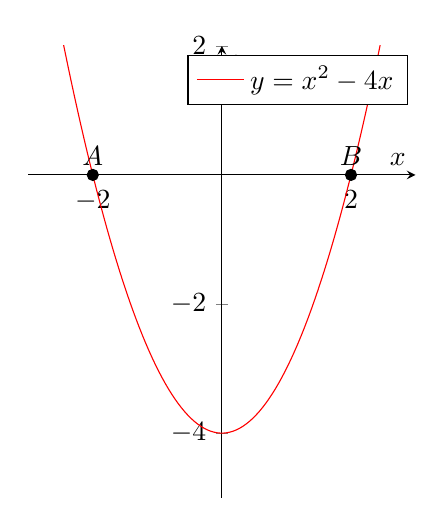
\begin{tikzpicture}
\begin{axis}[
    axis lines = middle,
    xlabel = $x$,
    ylabel = $y$,
    xmin=-3, xmax=3,
    ymin=-5, ymax=2,
    %legend pos = north west,
    axis equal image,
    width=0.7\textwidth
]


%\addplot[black, dashed, thick, domain=-4:4, samples=200] {x^3-4*x+2};
%\addlegendentry{$m=2$}

% Parabel
\addplot[red, domain=-5:5, samples=200] {x^2-4};
\addlegendentry{$y=x^2-4x$}

\addplot[only marks, mark=*, mark size=2pt] coordinates {(-2,0)};
\node[above] at (axis cs:-2,0) {$A$};

\addplot[only marks, mark=*, mark size=2pt] coordinates {(2,0)};
\node[above] at (axis cs:2,0) {$B$};

\end{axis}
\end{tikzpicture}
\end{center}
Analytisch ermitteln wir die Nullstelle durch das Einsetzen von $y=0$: 

\[ 0 = x^2 -4 \Leftrightarrow 4 = x^2 \Leftrightarrow \sqrt{4} = \pm x \Leftrightarrow x_{1/2}=\pm 2  \]
\end{example}

Schauen wir uns im Folgenden die Funktionen $f(x)=x^3$ und $g(x)=x^4$ an. Plotten wir die Funktionen, so fällt ein grundlegender Unterschied auf. Wir können $f(x)$ um $\ang{180}$ um den Koordinatenursprung $U(0|0)$ drehen, und erhalten den gleichen Funktionsgraphen wieder. $g(x)$ dagegen scheint \textit{Achsensymmetrisch} zur $y$-Achse. Spiegeln wir den Graphen an der $y$-Achse, so erhalten wir genau den anderen \glqq Ast\grqq der Funktion. Das kann man sich auch an der Funktionsgleichung überlegen. 
Eine Punktspiegelung um den Ursprung bedeutet nichts weiter als dass ich jeden Funktionswert $f(x)$ betrachte. Nun sehen wir, dass jedes Paar $(x|f(x))$ einen Spiegelpunkt bei $(-x|f(-x))$ hat. Wir entdecken für $f(x)$ den Punkt $P(1|1)$ und den Punkt $P'(-1|-1)$, wobei $f(-1)=-1 \cdot f(1)$ ist. 

\begin{definition}
Eine Funktion heißt \textbf{Punktsymmetrisch zum Ursprung}\index{Funktion!Symmetrie}\index{Funktion!Punktsymmetrisch}\index{Symmetrie einer Funktion}, wenn gilt:

\[ f(x) = - f(-x)\]

Sie heißt hingegen \textbf{achsensymmetrisch zur y-Achse}\index{Funktion!Achsensymmetrisch}, wenn gilt:

\[ f(x)= f(-x)\]
\end{definition}

\glqq Der Unterricht ist voll monoton!\grqq \ Wir verwenden das Wort \glqq monoton\grqq \ häufig im Alltag, und meinen damit, dass etwas sehr langanhaltend ist, es zieht sich. Bei Funktionen gibt es eine ähnliche Interpretation des Begriffes.

\begin{definition}
Für eine Funktion $f$ heißt das Intervall $[a,b]$
\index{Funktion!Monotonie} \index{Monotonie einer Funktion}
\begin{center}
\begin{tabular}{p{7cm} p{3cm}}
\renewcommand{\arraystretch}{1.7}
\textit{monoton steigend}, falls & $f(x_1)\leq f(x_2)$ \\
\textit{streng monoton steigend}, falls & $f(x_1)<f(x_2)$ \\
\textit{monoton fallend}, falls & $f(x_1)\geq f(x_2)$ \\
\textit{streng monoton fallend}, falls & $f(x_1)>f(x_2)$ \\
\end{tabular}
\end{center}
für alle $x_1, x_2\in [a,b]$ mit $x_1<x_2$ gilt.

\end{definition}

\begin{example}
Betrachten wir die Funktion $f(x)=x^2$ mit $D_f=\R$, so ist die Funktion auf ihrem gesamten Definitionsbereich \textbf{nicht} monoton. Schränken wir die Untersuchung auf das Intervall $I_1=[0,\infty[$ ein, so ist $f(x)$ streng monoton steigend, da für größere $x$-Werte auch die $y$-Werte steigen. \par
Wie sieht es mit dem Intervall $I_2=]-\infty, 0]$ aus?
\end{example}

Eine weitere wichtige Eigenschaft für Funktionen ist die \textbf{Periodizität}. Sie kennen wir hauptsächlich vom Sinus und Kosinus. 

\begin{theorem}
Für die allgemeine Sinus-Funktion $y=a\cdot \sin (b\cdot x - c)+d$ bzw. die allgemeine Kosinus-Funktion $y=a\cdot \cos (b\cdot x - c)+d$ gilt für die Periode $p$:
\[ p = \dfrac{2\pi}{b} \Leftrightarrow b = \dfrac{2\pi}{p} \]
Ist also $b$ gegeben, können wir stets die Periode ermitteln.
\label{Periode_SinCos}
\index{Funktion!Periode} \index{Periodizität einer Funktion}
\end{theorem}

Wie schon in Definition \ref{Def:Funktion} gesehen, ordnet eine Funktion $y=f(x)$ jedem $x\in D_f$ genau einen Funktionswert $y\in W_f$ zu. Manchmal sucht man aber zu einem $y$-Wert den passenden $x$-Wert.

\begin{definition}
Eine Funktion heißt \textit{umkehrbar}, wenn aus $x_1 \neq x_2$ stets $f(x_1) \neq f(x_2)$ folgt. Anders könnte man sagen, zu jedem Funktionswert $y$ gibt es genau einen $x$-Wert. \par
Ist eine Funktion $f$ umkehrbar, so nennen wir $f^{-1}$ die \textbf{Umkehrfunktion} von $f$. Sie ordnet jedem Wert der Wertemenge $W_f$ von $f$ den passenden Wert aus der Definitionsmenge $D_f$ von $f$ zu.
\index{Funktion!Umkehrfunktion} \index{Umkehrfunktion}
\end{definition}

\begin{theorem}
\textbf{(Vorgehen zum Bestimmen der Umkehrfunktion)}
\begin{enumerate}
\item Man löst die Funktionsgleichung $y=f(x)$ nach $x$ auf und erhält so $x=f^{-1}(y)$
\item Durch Vertauschen der beiden Variablen gewinnt man die Umkehrfunktion $y=f^{-1}(x)$
\end{enumerate}
Dabei vertauschen sich Wertemenge und Definitionsmenge: $D_f=W_f^{-1}$ und $W_f=D_f^{-1}$ \par
\textit{Bemerkungen:}
\begin{enumerate}[(1)]
\item Die Reihenfolge der Schritte ist egal.
\item Eine Funktion ist dort umkehrbar, wo sie streng monoton steigt (oder fällt).
\end{enumerate}
\end{theorem}

\begin{example}
Betrachten wir die lineare Funktion $f(x)=2x$ (rot). Das Umstellen nach $x$ liefert uns: $x=\dfrac{1}{2}y$. Nach dem Variablentauschen erhalten wir also: $f^{-1}(x)=\dfrac{1}{2}x$. Grafisch bedeutet das Bilden der Umkehrfunktion (blau) das Spiegeln an der Winkelhalbierenden.


\begin{center}
\begin{tikzpicture}[domain=-2:2]

	\draw[->] (-2.3,0) -- (2.3,0) node[right] {$x$};
	\draw[->] (0,-4.5) -- (0,2) node[above] {$f(x)$};
	\draw[color=red]	plot (\x, {2*\x})	node[right]	{$f(x)=2x$};
	\draw[color=blue]	plot (\x, {0.5 * \x})	node[right]	{$f(x)^{-1}=\dfrac{1}{2}x$};
	\draw[thick, dashed, color=black]	plot (\x, {\x})	node[right]	{Winkelhalbierende};
\end{tikzpicture}
\end{center}
\end{example}

Funktionen haben an bestimmten Stellen oft ein charakteristisches Verhalten. Für die Mathematik, aber auch oft in Sachzusammenhängen, sind dabei vor allem die Verläufe von Funktionen gegen $\infty$ und $-\infty$ relevant. Dafür nutzt man den Begriff des Grenzwertes:

\begin{definition}
Der Grenzwert $b$ ist derjenige Wert, dem sich die Funktion $f(x)$ in der Umgebung der Stelle $a$ annähert. Man schreibt:
\[ \lim_{x\rightarrow a} = b\]
\index{Grenzwert einer Funktion} \index{Funktion!Grenzwert}
\end{definition}

\begin{example}
Neben endlichen Grenzwerten gibt es auch unendliche. 
\begin{enumerate}
\item Eine endliche Grenzwertbetrachtung wäre der Grenzwert von $\lim_{x\to 4}x^2 = 16$, weil sich die Funktion $y=x^2$ in der Umgebung von $x=4$ dem Wert $y=16$ immer weiter annähert.
\item Betrachtet man $\lim_{x\to -\infty}e^x = 0$, so erhält man $0$, weil für sehr sehr kleine Werte ($x\to - \infty$) die Funktion $y=e^x$ dem Wert $0$ immer näher kommt. Dafür muss die Funktion selbst aber nicht zwingend $0$ sein, wie aus dem Beispiel hervorgeht.
\item Für dieselbe Funktion wie aus 2. erhalten wir $\lim_{x\to +\infty}e^x = \infty$, da für große $x$-Werte auch die $y$-Werte immer größer werden, und dabei unendlich groß werden. Es gibt also keine feste Obergrenze: Der Grenzwert für $y=e^x$ für $x$ gegen unendlich ist unendlich.
\end{enumerate}
\end{example}

Eine oftmals am Rande erwähnte Eigenschaft von Funktionen ist die Stetigkeit. In Jahrgangsstufe 11 hat man hierzu Sprungstellen etc. kennengelernt. Diese Begriffe wollen wir im Folgenden nochmals präzise benennen:

\begin{definition}
\index{Funktion!Stetigkeit} \index{Stetigkeit einer Funktion}
Eine Funktion $y=f(x)$ heißt stetig, wenn der Grenzwert 
\[ \lim_{x \rightarrow x_0} f(x) = f(x_0)\]
ist. Das bedeutet, dass man sich bei der Annäherung an den Wert $x_0$ von beiden Seiten an den selben Grenzwert, nämlich $x_0$ selbst, annähert.
\end{definition}

\begin{example}
Wir wollen uns nun zwei Funktionen und deren Stetigkeit ansehen.
\begin{enumerate}
\item Die Funktion $f(x)=x^2$ hat an der Stelle $x_0=1$ den Funktionswert $f(1)=1^2=1$, und der (beidseitige) Grenzwert ist genau $\lim_{\rightarrow 1} f(x)=1$. Man spricht von einer stetigen Funktion, weil die Funktion für jeden $x$-Wert stetig ist.
\item Die Funktion $h(x)=\begin{cases} 1 & x \leq 0 \\ 0 & x>0   \end{cases}$ ist an der Stelle $x=0$ nicht stetig, da der Grenzwert von links gleich $1$ ist, und von rechts kommend ist der Grenzwert $0$. Man spricht hierbei von einer Sprungstelle bei $x=0$, weil der Graph der Funktion hier schlagartig nach unten springt.

\begin{center}
\begin{tikzpicture}[domain=-4:4]

	\draw[->] (-4,0) -- (4,0) node[right] {$x$};
	\draw[->] (0,-1) -- (0,2) node[above] {$f(x)$};
	\draw[color=blue, domain=-4:0]	plot (\x, {1});
	\draw[color=blue, domain=0:+4]	plot (\x, {0})	node[above]	{$h(x)$};
	\draw[color=black]	plot[only marks, mark=*, mark size = 2pt]	coordinates{(0,0)};
	\draw[color=black]	plot[only marks, mark=*, mark size = 2pt, mark options={fill=white}]	coordinates{(0,1)};
\end{tikzpicture}
\end{center}
\item Die Funktion $y=\frac{1}{x}$ ist an der Stelle $x=0$ nicht stetig. Die Funktion ist an dieser Stelle nicht definiert, aber auch die Grenzwerte links und rechts der $0$ sind verschieden. (Übung)
\end{enumerate}
\end{example}

Oftmals reicht uns die Betrachtung der Stetigkeit aus, doch manchmal müssen wir sogenannte \textit{Unstetigkeitsstellen}, also Stellen, an denen die betrachtete Funktion nicht stetig ist, genauer betrachten. Dabei treffen wir folgende Unterscheidung:

\begin{definition}
Eine Funktion $y=f(x)$ heißt an der Stelle $x_0$ \textbf{unstetig}, wenn mindestens eine der drei Bedingungen erfüllt ist:
\begin{enumerate}
\item $f(x)$ ist für $x=x_0$ nicht definiert: $x_0 \notin D_f$
\item Der Grenzwert von $f(x)$ ist an der Stelle $x_0$ nicht vorhanden.
\item Funktionswert $f(x_0)$ und Grenzwert $g$ sind vorhanden, aber verschieden.
\end{enumerate}
\end{definition}

\begin{example}
Für die Unstetigkeit gibt es zwei wichtige Fälle:

\begin{enumerate}
\item Betrachten wir die gebrochen-rationale Funktion $f(x)=\frac{x^2-1}{x+1}$, so sehen wir an der Stelle $x_0=-1$ eine Definitionslücke, also ist $f$ dort unstetig. Durch Kürzen des Bruches können wir diese Definitionslücke aber beseitigen, wir erhalten:
\[ \dfrac{x^2-1}{x+1} = \dfrac{(x+1)(x-1)}{x-1} = x-1,\]
wobei wir zuerst die dritte binomische Formel genutzt haben, und dann \glqq gekürzt\grqq \ haben. Diese Form der Unstetigkeit nennt man \textbf{hebbare Lücke}.
\item Für $y=\dfrac{1}{(x-3)^2}$ lässt sich die Definitionslücke nicht beheben. Die Grenzwerte links- und rechtsseitig verlaufen für $x\to 3$ gegen $+\infty$. Man nennt $x_0=3$ deshalb auch \textbf{Polstelle}.
\end{enumerate}
\end{example}

\begin{definition}
Asymptoten sind Geraden, denen sich Funktionsgraphen annähern: 
\begin{enumerate}
\item \textbf{Senkrechte Asymptoten}\index{Senkrechte Asymptoten} sind geraden, die parallel zur $y$-Achse verlaufen. Sie werden über die Gleichung $x=x_S$ angegeben, wenn $x_S$ der $x$-Wert ist, an dem die Funktion eine Polstelle hat.
\item \textbf{Waagrechte Asymptoten}\index{Waagrechte Asymptoten} sind Geraden parallel zur $x$-Achse. Man kann sie durch die Gleichung $y=x_W$ ausdrücken. Wichtig hierbei: Die Funktion muss sich für $x\to \infty$ oder $x\to -\infty$ der Geraden annähern ($\rightarrow$ Grenzwert). Ob der Funktionsgraph die Asymptote schneidet, ist für die Asymptote nicht von Bedeutung.
\item \textbf{Schräge Asymptoten}\index{Schräge Asymptoten} lassen sich mit der Geradengleichung 
\[ g(x)=mx+t\]
darstellen. Wichtig: $m\neq 0$, sonst wäre die Asymptote eine waagerechte Asymptote. Ähnlich wie bei selbigen nutzt man auch bei schrägen Asymptoten die Grenzwertbetrachtungen. Gilt 
\[ \lim_{x\to \infty} f(x) = g\]
oder 
\[ \lim_{x\to -\infty} f(x) = g,\]
so besitzt $f(x)$ die schräge Asymptote $g$, die durch $y=g(x)$ beschrieben werden kann.
\end{enumerate}
\index{Funktion!Asymptoten} \index{Asymptoten einer Funktion}

\end{definition}

Als nächstes schauen wir uns Funktionen mit Parametern an, sogenannte Funktionsscharen. Sie sind Funktionen vom selben Typ, die durch Parameter geändert werden können:

\begin{definition}
Sei $f$ eine Funktion und $a\in \R$ beliebig. Dann heißt die Menge aller Funktionen 
\[ f_a : x \mapsto f_a(x)\]
\textbf{Funktionenschar} \index{Funktion!Schar} und $a$ wird als \textbf{Parameter}\index{Parameter} bezeichnet. 
\label{Def:Funktionenschar}
\end{definition}

\begin{example} \
\begin{enumerate}
\item Betrachten wir zuerst die Funktionenschar $f_a(x)=x^2-a\cdot x +2$. So können wir konkrete \glqq Vertreter\grqq \ der Funktion erhalten, indem wir beliebige $a$ einsetzen. So erhalten wir beispielsweise
\[ f_1(x)=x^2-x+2 \hspace{1cm} \text{und} \hspace{1cm} f_{-3}(x)=x^2+3x+2.\]
Graphisch sehen die Funktionen alle sehr ähnlich aus:
\begin{center}
\begin{tikzpicture}
\begin{axis}[
    axis lines = middle,
    xlabel = $x$,
    ylabel = $y$,
    xmin=-3, xmax=4,
    ymin=-1, ymax=8,
    legend pos = north west,
    axis equal image,
    width=\textwidth
]
\addplot[blue, dashed, domain=-3:4, samples = 200] {x^2-x+2};
\addlegendentry{$f_1(x)$}
\addplot[red, dashed, domain=-3:4, samples = 200] {x^2+3*x+2};
\addlegendentry{$f_{-3}(x)$}
\addplot[violet, dashed, domain=-3:4, samples = 200] {x^2-2*x+2};
\addlegendentry{$f_{2}(x)$}
\end{axis}
\end{tikzpicture}
\end{center}
\item Für die Funktionenschar $g_b(x)=e^{bx}$ sehen ausgewählte Graphen wiefolgt aus:
\begin{center}
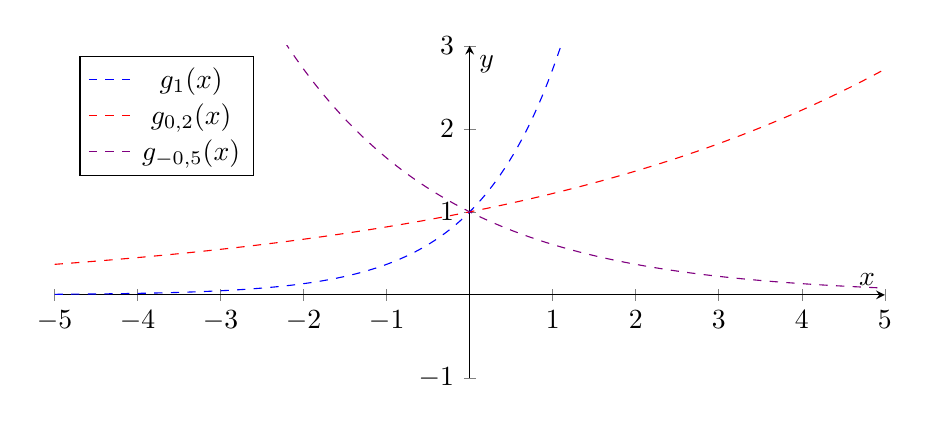
\begin{tikzpicture}
\begin{axis}[
    axis lines = middle,
    xlabel = $x$,
    ylabel = $y$,
    xmin=-5, xmax=5,
    ymin=-1, ymax=3,
    legend pos = north west,
    axis equal image,
    width=\textwidth
]
\addplot[blue, dashed, domain=-5:5, samples = 200] {e^x};
\addlegendentry{$g_1(x)$}
\addplot[red, dashed, domain=-5:5, samples = 200] {e^((0.2)*x)};
\addlegendentry{$g_{\num{0,2}}(x)$}
\addplot[violet, dashed, domain=-5:5, samples = 200] {e^((-0.5)*x)};
\addlegendentry{$g_{-\num{0,5}}(x)$}
\end{axis}
\end{tikzpicture}
\end{center}
\end{enumerate}
\end{example}

Manchmal kommt es vor, dass man eine Funktion hat, deren Funktionswert man in eine andere Funktion einsetzt. Man spricht hierbei von der Verkettung von Funktionen.

\begin{definition}
Seien $f$ und $g$ zwei Funktionen, dann heißt die Funktion
\[ (f\circ g)(x) = f(g(x))\]
\textbf{Verkettung} der Funktionen $f$ und $g$. \index{Verkettung von Funktionen} \index{Funktion!Verkettung von}
\end{definition}

\begin{theorem}
Die Verkettung $f\circ g$ ist im Allgemeinen nicht kommutativ: $f\circ g \neq g \circ f$.
\end{theorem}

\begin{example}
Gegeben ist die Funktion $f(x)=x^2$ und die Funktion $g(x)=e^x$. Wir bilden nun die Verkettungen der Funktionen:
\[ (f\circ g)(x)= f(g(x))=f(e^x) = \mleft( e^x \mright)^2 = e^{2x} \hspace{1cm} \text{und} \hspace{1cm} (g\circ f)(x)= g(x^2)=e^{x^2} \]
Betrachten wir die Graphen von $g$ und $f$.
\begin{center}
\begin{tikzpicture}
\begin{axis}[
    axis lines = middle,
    xlabel = $x$,
    ylabel = $y$,
    xmin=-5, xmax=5,
    ymin=-1, ymax=4,
    legend pos = north west,
    axis equal image,
    width=\textwidth
]
\addplot[blue, domain=-5:5, samples = 200] {x^2};
\addlegendentry{$f(x)=x^2$}
\addplot[red, domain=-5:5, samples = 200] {e^x};
\addlegendentry{$g(x)=e^x$}
\end{axis}
\end{tikzpicture}
\end{center}
Den Funktionswert $(f\circ g)(-2)$ erhalten wir, indem wir uns nochmals in Erinnerung rufen, dass dies bedeutet: $f(g(-2))$. Wir bestimmen deshalb zuerst den Funktionswert von $g$ an der Stelle $x=-2$: $g(2) \approx \num{0,1}$. Nun haben wir den Funktionswert von $g(-2)$, den wir in $f$ einsetzen müssen. Graphisch lesen wir deshalb nun an der x-Stelle $x=\num{0,1}$ den Funktionswert von $f$ ab: $f(\num{0,1})\approx \num{0,01}$. 
\end{example}
\newpage

\subsection{Arten von Funktionen}

%\subsubsection{Lineare Funktionen}
\begin{definition}
\index{Funktion!Lineare Funktionen} \index{Lineare Funktionen}
Lineare Funktionen sind Geraden im Koordinatensystem. Sie werden beschrieben durch
\[ f(x)=mx+t\]
Dabei ist $m$ die Steigung und $t$ der $y$-Achsenabschnitt. Die Steigung ist an jeder Stelle der Funktion gleich.

\begin{center}
\begin{tikzpicture}
\begin{axis}[
    axis lines = middle,   % Achsen durch den Ursprung
    xlabel = $x$,
    ylabel = $f(x)$,
    xmin=-5, xmax=5,
    ymin=-2, ymax=8,
%    grid = both,           % optional
]
\addplot[blue, domain=-5:5] {x+3};
\addplot[red, domain=-5:5] {0.5*x+2};
\end{axis}
\end{tikzpicture}
\end{center}
\end{definition}

%\subsubsection{Quadratische Funktionen}
\begin{definition}
\index{Funktion!Quadratische Funktionen} \index{Quadratische Funktionen}
Quadratische Funktionen sind Parabeln. Man kann quadratische Funktionen auf drei Arten angeben:
\begin{enumerate}
\item $f(x)=ax^2+bx+c$ (Normalform) \index{Normalenform der quadrat. Funktion}
\item $f(x)=a(x-x_S)^2+y_S$ (Scheitelpunktform), wobei $S(x_S|y_S)$ der Scheitelpunkt ist. \index{Scheitelpunktform}
\item $f(x)=a(x-x_1)\cdot (x-x_2)$ (faktorisierte Form oder Nullstellenform), wobei $x_{1/2}$ die Nullstellen sind. \index{Faktorisierte Form}
\end{enumerate}
Die spezielle quadratische Form $y=x^2$ heißt \textit{Normalparabel}. \index{Normalparabel}
\end{definition}


\begin{example} \ \par
\begin{center}
\begin{tikzpicture}
\begin{axis}[
    axis lines = middle,
    xlabel = $x$,
    ylabel = $y$,
    xmin=-5, xmax=5,
    ymin=-2, ymax=8,
    legend pos = north west
]
\addplot[blue, domain=-5:5, samples=200] {x^2-2*x};
\addlegendentry{$y=x^2-2x$}
\end{axis}
\end{tikzpicture}
\end{center}
Die drei Formen lauten in diesem Beispiel:
\[ f(x)= \frac{1}{2}x^2 -2x = \frac{1}{2}(x-2)^2-2 = \frac{1}{2} (x-0) \cdot (x-4) \]
\end{example}

\begin{theorem} \textbf{(Über die Nullstellen einer quadratischen Funktion)} \par
\begin{enumerate}
\item Falls für die \textbf{Diskriminante} $\sqrt{b^2-4ac}$ gilt:
	\begin{itemize}
	\item $b^2-4ac>0$, dann hat $f(x)$ zwei Nullstellen,
	\item $b^2-4ac=0$, dann hat $f(x)$ genau eine Nullstelle, und
	\item $b^2-4ac<0$, dann besitzt $f(x)$ keine Nullstellen.
	\end{itemize}
\index{Mitternachtsformel} \index{Lösungsformel für quadrat. Funktionen}
\item Für die Bestimmung der Nullstellen nutzen wir die Mitternachtsformel. In der Normalform gilt:
\[ x_{1/2}=\dfrac{-b\pm\sqrt{b^2-4ac}}{2a} \]

\end{enumerate}



\end{theorem}

%\subsubsection{Polynomfunktionen}
\begin{definition}
Eine Funktion vom Typ $f(x)=a_nx^n + a_{n-1}x^{n-1} + ... + a_1 \cdot x + a_0$ nennen wir Polynomfunktion. Der größte Exponent $n$ heißt hierbei \textit{Grad} des Polynoms bzw. der ganzrationalen Funktion.
\index{Polynomfunktion} \index{Funktion!Polynomfunktion} \index{Ganzrationale Funktion} \index{Funktion!Ganzrationale}
\end{definition}

\begin{example}
Die Funktion $y=3x^2-4x^5+20$ ist eine Polynomfunktion vom Grad $n=5$, denn der größte Exponent ist hier die Zahl $5$.
\end{example}

%\subsubsection{Gebrochen-rationale Funktionen}
In den vorherigen Kapiteln haben wir uns angeschaut, wie sich Funktionen verhalten, die das $x$ im Zähler haben. Doch auch Funktionen, die die Variable im Nenner haben, sind denkbar. Die einfachste Form ist wohl $f(x)=\frac{1}{x}$. Im Allgemeinen kannst du dir gebrochen rationale Funktionen als Quotient oder Bruch zweier Polynomfunktionen vorstellen. 

\begin{definition}
Eine gebrochen-rationale Funktion ist allgemein in der Form
\[ f(x)=\dfrac{g(x)}{h(x)} \]
darstellbar, wobei $g$ und $h$ beliebige Polynomfunktionen sein können.
\index{Gebrochen-rationale Funktion} \index{Funktion!Gebrochen-rationale Funktion}
\end{definition}

\begin{example}
Das einfachste Beispiel stellt die Funktion $y=\dfrac{1}{x}$ dar:

\begin{center}
\begin{tikzpicture}
\begin{axis}[
    axis lines = middle,
    xlabel = $x$,
    ylabel = $y$,
    xmin=-5, xmax=5,
    ymin=-3, ymax=3,
    unbounded coords=jump
]
\addplot[blue, domain=-5:5, samples = 200] {x == 0 ? nan : 1/x};
%\addlegendentry{$y=\frac{1}{x}$}
\end{axis}
\end{tikzpicture}
\end{center}

\end{example}

Die Definitionslücke bei $x=0$ ist auf die Nullstelle von $y=x$ (der Funktion im Nenner) zurückzuführen. Das führt uns zu einem Vorgehen:

\begin{theorem}

Gebrochen-rationale Funktionen haben genau dort eine Definitionslücke, wo das Nennerpolynom $h(x)$ eine Nullstelle besitzt. 
\index{Definitionslücke}
\end{theorem}

\begin{example}

Die Funktion $y=\dfrac{4x^2-3x+3}{2x^2-1}$ hat genau bei $x=\pm \dfrac{\sqrt{2}}{2}$ zwei Definitionslücken, weil die Nullstellen des Nennerpolynoms $h(x)=2x^2-1$ dort liegen. \par
\textit{Übung:} Bestimme die waagerechten und senkrechten Asymptoten. Ermittle den links- und rechtsseitigen Grenzwert zu den senkrechten Asymptoten. (Lösung zum Beispiel in GeoGebra)

\end{example}

Um festzustellen, wo und ob eine gebrochen-rationale Funktion eine waagrechte Asymptote besitzt, muss man sich den Grad des Nennerpolynoms $n$ und den Grad des Zählerpolynoms $z$ anschauen. Grad meint hierbei jeweils die größte Potenz. Dabei gilt folgender Zusammenhang:

\begin{theorem} \textbf{(Waagrechte Asymptoten bei gebrochen-rationalen Funktionen)} \par
Sei $f(x)=\dfrac{g(x)}{h(x)}$ eine gebrochen-rationale Funktion, wobei der Grad des Zählerpolynoms mit $z$ beschrieben wird. Das Nennerpolynom ist vom Grad $n$. Dann gilt:
\begin{enumerate}
\item $\mathbf{z=n}$: Sind Zähler- und Nennerpolynom vom selben Grad, so gibt es eine waagrechte Asymptote: 
\[ f(x) = \dfrac{g(x)}{h(x)} = \dfrac{a_nx^n+...+a_1x+a_0}{b_nx^n+...+b_1x+b_0} \Rightarrow \text{waagrechte Asymptote bei} \ y=\dfrac{a_n}{b_n}\]
\item $\mathbf{z<n}$: Ist der Nennergrad größer als der Zählergrad, so gibt es eine waagrechte Asymptote bei $y=0$.
\item $\mathbf{z>n}$: Ist der Zählergrad größer als der Nennergrad, so liegt \textbf{keine} waagrechte Asymptote vor.
\item Sonderfall: Falls $z=n+1$ gilt, der Zählergrad also um $1$ größer ist als der Nennergrad, so existiert eine \textbf{schräge Asymptote}.
\end{enumerate}
\label{Satz:Waag_Asympt}
\index{Waagrechte Asymptoten bei gebr.-rat. Funktionen} \index{Asymptoten!bei gebr.-rat. Funktionen}
\end{theorem}

\begin{example} Für jeden der vier Fälle betrachten wir eine Funktion:

\begin{enumerate}
\item Sei $f(x)=\dfrac{3x^2-4x+1}{2x^2-4}$, so liegt nach Satz \ref{Satz:Waag_Asympt} 1. bei $y=\dfrac{3}{2}$ vor. Graphisch bestätigen wir diese Vermutung:
\begin{center}
\begin{tikzpicture}
\begin{axis}[
    axis lines = middle,
    xlabel = $x$,
    ylabel = $y$,
    xmin=-7, xmax=7,
    ymin=-3, ymax=5,
    unbounded coords=jump,
    samples=300,
    width = 14cm,
    height = 9cm
]

% links der Polstelle
\addplot[blue, domain=-7:-1.5]
{(3*x^2 - 4*x + 1)/(2*x^2 - 4)};
\addlegendentry{$y=\frac{3x^2-4x+1}{2x^2-4}$}

% zwischen den Polstellen
\addplot[blue, domain=-1.3:1.36]
{(3*x^2 - 4*x + 1)/(2*x^2 - 4)};

% rechts der Polstelle
\addplot[blue, domain=1.47:7]
{(3*x^2 - 4*x + 1)/(2*x^2 - 4)};

% waagrechte Asymptote
\addplot[red, dashed, domain=-7:7] {3/2};

\end{axis}
\end{tikzpicture}
\end{center}
Analytisch können wir das nachrechnen, indem wir die größte Potenz $x^2$ im Zähler und Nenner ausklammern und den Grenzwert für $\pm \infty$ untersuchen. Dafür nutzen wir aus, dass für $x\neq 0$ gilt: $\dfrac{x^2}{x^2}=1 \ (1)$. Exemplarisch für $x\to \infty$ ergibt sich:
\[ \lim_{x\to \infty} \dfrac{3x^2-4x+1}{2x^2-4} = \lim_{x\to \infty} \dfrac{x^2 \mleft( 3-\frac{4}{x}+\frac{1}{x^2}    \mright)}{x^2 \mleft( 2-\frac{4}{x^2} \mright)} =  \lim_{x\to \infty} \dfrac{x^2 \mleft( 3-0+0 \mright)}{x^2 \mleft( 2-0 \mright)} \stackrel{(1)}{=} \dfrac{3}{2} \]
\item Betrachten wir die Funktion $g(x)=\dfrac{1}{x^2+1}$. So gilt für die waagrechte Asymptote $y=0$. Es ist eine gute Übung, das graphisch zu zeichnen und nachzurechnen mithilfe des Limes.
\item Sei $h(x)=\dfrac{4x^4+3x-1}{2x^2+1}$. Nach Satz \ref{Satz:Waag_Asympt} 3. existiert hier keine waagrechte Asymptote. (Übung)
\item Für $k(x)=\dfrac{3x^3+2x-1}{2x^2+5}$ muss nach Satz \ref{Satz:Waag_Asympt} 4. eine senkrechte Asymptote existieren, da der Zählergrad um eins höher als der Nennergrad ist. Durch nachrechnen ergibt sich:
\[ \lim_{x\to \infty} \dfrac{3x^3+2x-1}{2x^2+5} = \lim_{x\to \infty} \dfrac{x \cdot \mleft(3 x^2+2-\frac{1}{x}\mright)}{2x^2+5} = \lim_{x\to \infty} x \cdot \dfrac{3x^2+2-0}{2x^2+5}  \]
\[ \stackrel{\text{Bsp. 1.}}{=} \lim_{x\to \infty} \frac{3}{2}x, \]
wobei im letzten Schritt wieder der Fall 1. Verwendung fand. Die schräge Asymptote ist also bei $y=\dfrac{3}{2}x$.
\end{enumerate}



\end{example}

%\subsubsection{Wurzelfunktionen}
Nachdem wir die Polynom-Funktionen bereits kennengelernt haben, erweitern wir diese Idee. Bisher hatten wir nur natürliche Exponenten zugelassen, doch im Folgenden wollen wir alle rationalen Exponenten zulassen:

\begin{definition}

Wurzelfunktionen sind Funktionen, die als Wurzel geschrieben werden können. Äquivalent dazu ist die Auffassung, dass wir die Funktion mit rationalem Exponenten schreiben.
\[ \sqrt{p(x)} = \mleft( p(x) \mright)^{\frac{1}{2}}  \]
wobei $p(x)$ eine beliebige Funktion ist. Eine Wurzelfunktion ist nur definiert, wenn der \textbf{Radikant} nicht-negativ ist, also $W_f=\R^+_0$ gilt. 
\index{Funktion!Wurzelfunktion} \index{Wurzelfunktion} \index{Radikant}
\end{definition}

\begin{example}
\ 
\begin{enumerate}
\item Die Funktion $y=\sqrt{x}$ ist die wohl einfachste Wurzelfunktion. Sie hat die Definitionsmenge von $D=\R_0^+$.

\begin{center}
\begin{tikzpicture}
\begin{axis}[
    axis lines = middle,
    xlabel = $x$,
    ylabel = $y$,
    xmin=-1, xmax=5,
    ymin=-1, ymax=3,
]
\addplot[blue, domain=0:5, samples = 200] {sqrt(x)};
\addlegendentry{$y=\sqrt{x}$}
\end{axis}
\end{tikzpicture}
\end{center}

\item Sei $y=\sqrt{2x+1}$ die betrachtete Wurzelfunktion, so gilt es nun, die Definitionsmenge zu bestimmen. Dafür muss $2x+1\geq 0$ gelten. Wir formen um zu:
\[ 2x+1\geq 0 \Leftrightarrow 2x \geq -1 \Leftrightarrow x \geq - \frac{1}{2}  \]
Daraus folgt, dass für $x\geq - \frac{1}{2}$ die Funktion definiert ist. Die Definitionsmenge ist also $D=\{ x \in \R | x \geq - \frac{1}{2}   \}$, oder in Worten: \textit{Alle reellen Zahlen $x$, für die gilt: $x$ ist größer oder gleich $-\frac{1}{2}$}.

\begin{center}
\begin{tikzpicture}
\begin{axis}[
    axis lines = middle,
    xlabel = $x$,
    ylabel = $f(x)$,
    xmin=-1, xmax=5,
    ymin=-1, ymax=5,
]
\addplot[blue, domain=-0.5:5, samples = 200] {sqrt(2*x + 1)};
\addlegendentry{$y=\sqrt{2x+1}$}
\end{axis}
\end{tikzpicture}
\end{center}
\end{enumerate}

\end{example}

Lässt man allgemein rationale Exponenten zu, so folgt daraus $y=\mleft( p(x) \mright) ^{\frac{n}{m}}, n,m \in \N$. 

%\subsubsection{Trigonometrische Funktionen}
Die drei trigonometrischen Funktionen aus der Schule sind der Sinus, Kosinus und der Tangens. Dabei leiten sich die Funktionen aus den Beziehungen im (rechtwinkligen) Dreieck her:
\begin{itemize}
\item $\sin \alpha = \dfrac{\mathrm{Gegenkathete}}{\mathrm{Hypotenuse}}$
\item $\cos \alpha = \dfrac{\mathrm{Ankathete}}{\mathrm{Hypotenuse}}$
\item $\tan \alpha = \dfrac{\sin \alpha}{\cos \alpha} = \dfrac{\mathrm{Gegenkathete}}{\mathrm{Ankathete}}$
\index{Sinus} \index{Kosinus} \index{Tangens}
\end{itemize}
Eine gute Merkhilfe stellt die \textbf{GAGA}-\textbf{H}ühner\textbf{H}of-\textbf{AG} dar:
\begin{tabular}{c c c c}
G & A & G & A\\
H & H & A & G \\
 & & & \\
\rotatebox{90}{$\sin x$} & \rotatebox{90}{$\cos x$} & \rotatebox{90}{$\tan x$} & \rotatebox{90}{$\tan ^{-1} x$}
\end{tabular}.\par
Die Überlegung am Dreieck führt auch zum Einheitskreis, an dem man Sinus und Kosinus gut darstellen kann:
\index{Einheitskreis}
\begin{center}
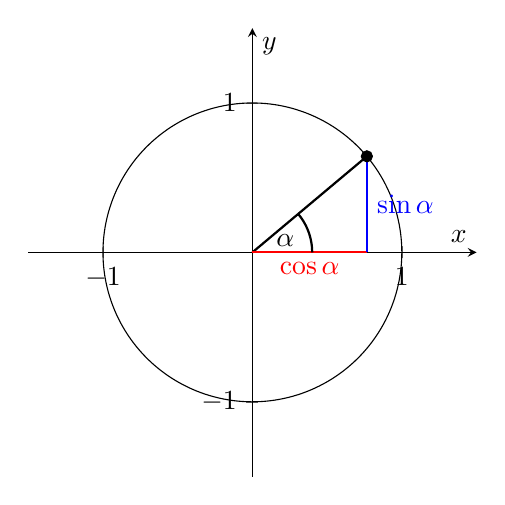
\begin{tikzpicture}
\begin{axis}[
    axis equal image,
    axis lines=middle,
    xmin=-1.5, xmax=1.5,
    ymin=-1.5, ymax=1.5,
    xtick={-1,0,1},
    ytick={-1,0,1},
    xlabel=$x$,
    ylabel=$y$
]

% Einheitskreis
\addplot[
  domain=0:360,
  samples=200
] ({cos(x)}, {sin(x)});

% Winkel in Grad
\def\winkel{40} 

% Punkt am Kreis
\addplot[mark=*] coordinates {({cos(\winkel)}, {sin(\winkel)})};

% Hypotenuse (schwarz)
\addplot[black, thick] coordinates {
  (0,0)
  ({cos(\winkel)}, {sin(\winkel)})
};

% Kosinus (rot, waagrecht)
\addplot[red, thick] coordinates {
  (0,0)
  ({cos(\winkel)},0)
} node[pos=0.5, below] {$\cos \alpha$};

% Sinus (blau, senkrecht)
\addplot[blue, thick] coordinates {
  ({cos(\winkel)},0)
  ({cos(\winkel)}, {sin(\winkel)})
} node[pos=0.5, right] {$\sin \alpha$};

% Winkel Alpha als Bogen
\addplot[domain=0:\winkel, samples=50, thick]	({0.4*cos(x)}, {0.4*sin(x)});

% Beschriftung Alpha
\node at (axis cs:0.22,0.08) {$\alpha$};

\end{axis}
\end{tikzpicture}
\end{center}
Da die Länge der Hypotenuse dem Radius des Kreises ($r=1$) entspricht, ist die Strecke der Ankathete von $\alpha$ gleich mit dem Kosinus. Ähnlich gilt für die Gegenkathete, dass sie gleich lang wie der $\sin \alpha$ ist. \par
Üblicherweise gibt man Winkel graphisch im Gradmaß\index{Gradmaß} mit Winkel $\alpha$ an, doch es gibt auch die Alternative mit dem \textbf{Bogenmaß}\index{Bogenmaß} $b$, für das gilt:
\[ b = \dfrac{\alpha \cdot 2 \pi}{ \ang{360}}\]
Daraus folgen insbesondere $\ang{360} \ \hat{=} \ 2\pi$ und $\ang{180} \ \hat{=} \ \pi$, deren Werte man sich merken sollte. Durch den Einheitskreis können wir die Winkel aber auf beliebig große Winkel erweitern, die wir im Bogenmaß als $x$-Werte einer Funktion interpretieren können.

\begin{definition}
Die Sinus- und Kosinus-Funktion sind trigonometrische Funktionen, die periodisch verlaufen.
\index{Funktion!Trigonometrische Funktionen} \index{Sinus} \index{Kosinus}
\begin{center}
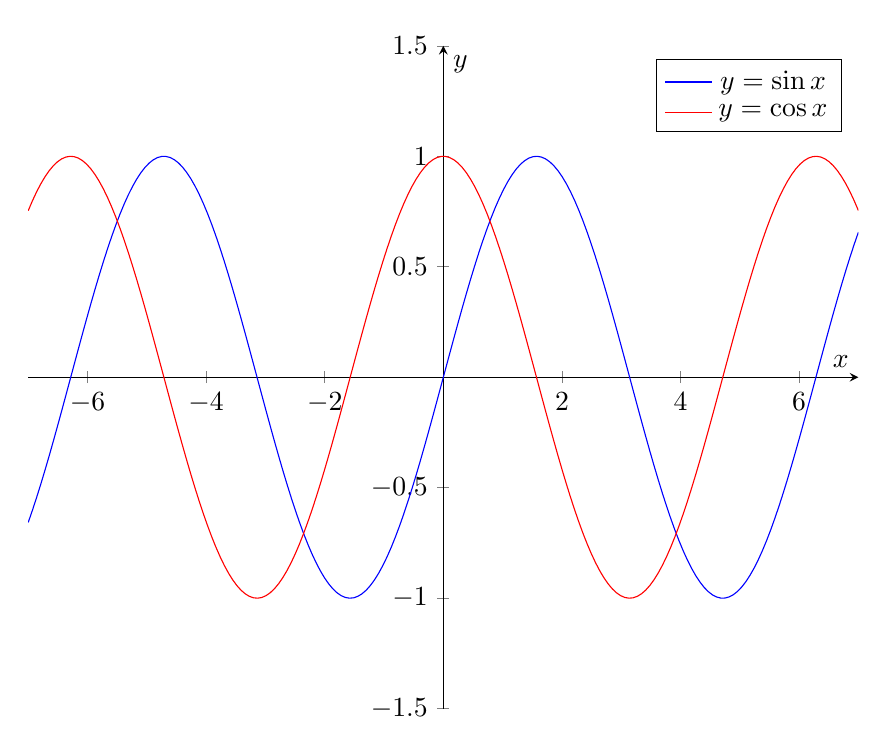
\begin{tikzpicture}
\begin{axis}[
    axis lines = middle,
    xlabel = $x$,
    ylabel = $y$,
    xmin=-7, xmax=7,
    ymin=-1.5, ymax=1.5,
    width=\textwidth,
    height=10cm,
]
\addplot[blue, domain=-7:7, samples = 200] {sin (deg(x))};
\addlegendentry{$y=\sin x$}
\addplot[red, domain=-7:7, samples = 200] {cos (deg(x))};
\addlegendentry{$y=\cos x$}
\end{axis}
\end{tikzpicture}
\end{center}

\end{definition}

Wir erkennen anhand des Graphen: Die Funktionen sind jeweils um $\frac{\pi}{2}$ zueinander verschoben. Wir fassen die wichtigsten Aussagen zusammen:
\begin{theorem} \textbf{(Eigenschaften der Sinus- und Kosinusfunktion)}
\begin{enumerate}
\item Der Definitionsbereich von $y=\sin x$ und $y=\cos x$ ist jeweils ganz $\R$,
\item Der Wertebereich ist ebenfalls identisch. Es gilt: $W_f = [-1;1]$.
\item Die Periode beider Funktionen ist $p=2\pi$.
\item Während $y=\sin x$ punktsymmetrisch zum Ursprung ist, ist $y=\cos x$ achsensymmetrisch zur $y$-Achse. 
\item Die Nullstellen der Sinusfunktion lauten für $k \in \Z$: $x_k=k \cdot \pi$. Für die Kosinusfunktion sind alle Nullstellen von der Form $x_k=\dfrac{\pi}{2}+k \cdot \pi$ darstellbar.
\item $\sin x = \cos \mleft( x-\dfrac{\pi}{2} \mright) \Leftrightarrow \cos x = \sin \mleft( x + \dfrac{\pi}{2}  \mright)$
\item Aus der Mittelstufe ist der \textit{trigonometrische Pythagoras}\index{Pythagoras!trigonometrischer} bekannt: Für alle $x\in \R$ gilt: $\sin^2 (x) + \cos^2 (x) = 1$. \footnote{Eine gute Übung ist es, diese Beziehung anhand des Einheitskreises herzuleiten.}
\end{enumerate}
\end{theorem}
Wichtig ist in diesem Zusammenhang auch nochmals Satz \ref{Periode_SinCos}, mit dem wir uns die Periode der beiden Funktionen im Allgemeinfall berechnen können.

%\subsubsection{Exponentialfunktionen}
In vielen Anwendungen wie Abklings-, Wachstums- oder Zerfallsprozessen spielen Exponentialfunktionen eine zentrale Rolle. Mit ihnen kann man Sachzusammenhänge präzise modellieren und dadurch berechenbar machen. Zuerst wollen wir uns dafür nochmals die Rechenregeln der \textbf{Potenzen} in Erinnerung rufen, die wir für Exponentialfunktionen oft brauchen. 

\begin{theorem} \ \par
\begin{tabularx}{\textwidth}{X X}
\setstretch{2}
\textbf{Rechenregeln für Potenzen} & \textbf{Zahlenbeispiele} \\
\\
1.   $a^m\cdot a^n=a^{m+n}$ & $2^3\cdot 2^2=2^{3+2} = 2^5 = 32$ \\
\\
2.   $\dfrac{a^m}{a^n}=a^{m-n}$ & $\dfrac{3^5}{3^7}=3^{5-7}=3^{-2}=\dfrac{1}{3^2}=\dfrac{1}{9}$ \\
\\
3.   $(a^m)^n=a{m\cdot n}$ & $(2^3)^5=2^{3\cdot 5}=2^{15}=32768$
\index{Potenzen}
\end{tabularx}
\end{theorem}

\begin{definition} Für die Potenz $a^x, a>0$ heißt die in den reellen Zahlen definierte Funktion $f(x)=a^x$ \textbf{Exponentialfunktion}.
\label{Def:Expon}
\index{Exponentialfunktion} \index{Funktion!Exponential}
\end{definition}

\begin{theorem} \textbf{(Satz über Exponentialfunktionen)}
\begin{enumerate}[1.]
\item Die Wertemenge einer Exponentialfunktion $f$ ist stets $W_f=\R^+$. 
\item Für $0<a<1$ ist $f$ streng monoton fallend. Für $a>1$ steigt die Funktion streng monoton.
\end{enumerate}
\label{Satz_Exponentialfunktion}
\end{theorem}

\begin{example} \

\begin{enumerate}
\item Betrachten wir die Funktion $f(x)=\mleft( \dfrac{2}{3} \mright)^x$, so wissen wir nach Satz \ref{Satz_Exponentialfunktion}, dass $f(x)$ streng monoton fallend sein muss. Ein Abgleich mit dem Graphen bestätigt uns das.
\item Die Funktion $g(x)=2^x$ ist streng monoton steigend.
\end{enumerate}
\begin{center}
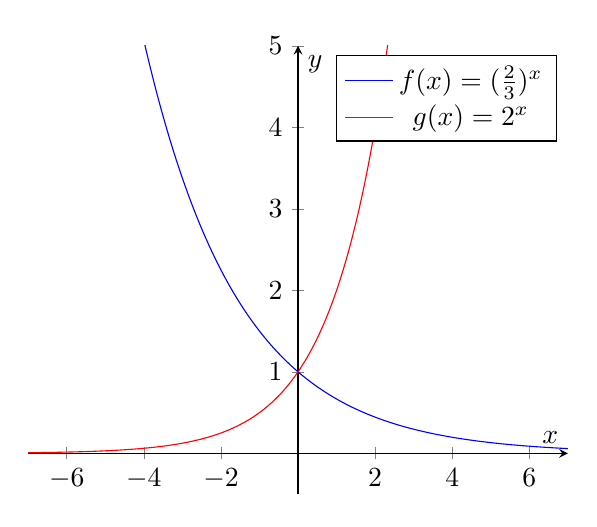
\begin{tikzpicture}
\begin{axis}[
    axis lines = middle,
    xlabel = $x$,
    ylabel = $y$,
    xmin=-7, xmax=7,
    ymin=-0.5, ymax=5,
   % width=\textwidth,
    %height=10cm,
]
\addplot[blue, domain=-7:7, samples = 200] {(2/3)^x};
\addlegendentry{$f(x)=\mleft( \frac{2}{3} \mright)^x$}
\addplot[red, domain=-7:7, samples = 200] {(2)^x};
\addlegendentry{$g(x)=2^x$}
\end{axis}
\end{tikzpicture}
\end{center}
\end{example}

Von besonderer Bedeutung ist die Exponentialfunktion 
\[ y=e^x \]
Dabei ist $e$ die \textit{Eulersche Zahl}, die durch den Grenzwert 
\[
e=\lim_{n\rightarrow \infty} \mleft( 1+\dfrac{1}{n}\mright) ^n = \num{2,718281}...
\]
definiert ist. Die Funktion $y=e^x$ nennen wir auch $e$-Funktion. Sie ist mit Abstand die wichtigste Exponentialfunktion. 
\begin{theorem} \
\begin{enumerate}
\item Jede Exponentialfunktion aus Definition \ref{Def:Expon} ist darstellbar als $f(x)=e^{\lambda\cdot x}$ mit $\lambda = \ln a$ (siehe Definition \ref{Def:Logarithmus}). 
\item Für $\lambda > 0$ ist die $e$-Funktion streng monoton steigend.
\item Ist $\lambda < 0$, so fällt die Funktion streng monoton. 
\end{enumerate}
\end{theorem}

%\subsubsection{Logarithmusfunktionen}
\begin{definition}
Die Lösung der Exponentialgleichung $r=a^x$ mit $r\in \R^+, a>0$ und $x\in \R$ bezeichnet man als \textbf{Logarithmus} von $r$. Man schreibt:
\[ x=\log_a(r)  \]
Der spezielle Logarithmus zur Gleichung $b=e^x$ mit $b \in \R^+, x\in \R$ heißt \textbf{natürlicher Logarithmus} mit 
\[ x= \log_e(b) = \ln b \]
\label{Def:Logarithmus}
\index{Logarithmus} \index{Natürlicher Logarithmus}
\end{definition}

\begin{theorem} \ \par

\begin{tabularx}{\textwidth}{X X}
\setstretch{2}
\textbf{Rechenregeln für Logarithmen} & \textbf{Zahlenbeispiele} \\
\\
1.   $\log_a (u\cdot v) = \log_a u + \log_a v$ & $\log_2 (8\cdot 4) = \log_2 8 + \log_2 4 = 3+2=5$ \\
\\
2.   $\log_a\mleft( \dfrac{u}{v} \mright) = \log_a u - \log_a v$ & $\log_3\mleft( \dfrac{81}{27} \mright) = \log_3 81 - \log_3 27=4-3=1$ \\
\\
3.   $\log_a u^n = n \cdot \log_a u$ & $\log_5 125^4 = 4 \cdot \log_5 125=4\cdot 3 = 12$ \\
\\
4.   $\log_a a^x = x \cdot \underbrace{\log_a a}_1 = x$ & $\ln e^x = x \underbrace{\ln e}_1 = x$ \\
\\
5.   $a^{\log_a x} = x$ & $e^{\ln x} = x$ \\
\\
6.   $\ln f(x) = \ln g(x) \Rightarrow f(x) = g(x)$ 

\end{tabularx}
\end{theorem}

Nun gehen wir analog wie bei den Exponentialfunktion vor: Wir ersetzen $b$ mit $x$ und erhalten die natürliche Logarithmusfunktion:

\begin{definition}

Die Funktion $y=\ln x$ heißt natürliche Logarithmusfunktion. \index{Funktion!Logarithmusfunktion} \index{Logarithmusfunktion}

\end{definition}

\begin{theorem} \textbf{(Eigenschaften der natürlichen Logarithmusfunktion)} \par
Nehme $f(x)=\ln x$ und $g(x)=e^x$. Dann gilt:
\begin{enumerate}
\item Die Definitionsmenge von $y=\ln x$ ist gleich mit der Wertemenge von $y=e^x$, die jeweils zueinander die Umkehrfunktion darstellen. Es gilt also $D_f = W_g=\R^+$.
\item Daraus folgt direkt: $W_f=D_g=\R$
\item $f(x)$ hat eine Nullstelle bei $x=1$, da $\ln 1 = 0$ ist.
\item Die $\ln$-Funktion ist streng monoton steigend.
\end{enumerate}
\label{Satz:E-Logarithmus}
\end{theorem}

\begin{example}
Wir betrachten im Folgenden die natürliche Logarithmusfunktion $f(x)=\ln (2x^2-2)$. Wegen Satz \ref{Satz:E-Logarithmus} 1. müssen wir $2x^2+2>0$ setzen. Da das für alle reellen Zahlen gilt, ist $D_f=\R^+$. Die Wertemenge hängt von der Wertemenge von $h(x)=2x^2+2$ ab, denn jeder $y$-Wert unserer Hilfsfunktion $h$ ergibt einen $y$-Wert von $f$ selbst. Für $W_h$ gilt $y\geq 2$ (Übung). Unsere Werte, die wir in $\ln x$ einsetzen, sind genau die $y$-Werte von $h$, also ist der kleinste Wert für unsere Funktion $f$ selbst $\ln 2$. Jeder andere Wert ist größer, und damit ist die Wertemenge von $f$ genau $W_f=\{ y \in \R | y \geq \ln 2  \}$. Da $1 \notin W_h$ liegt, hat $f$ auch keine Nullstellen. \par
\textit{Hinweis:} Dieses Beispiel ist schon sehr anspruchsvoll. Die eigenständige Lösung wird in der Schule vermutlich nicht erwartet. Als eigene Übung könnte man aber die vier Aspekte aus Satz \ref{Satz:E-Logarithmus} auf die Funktion $y=\ln (2x)$ anwenden.
\end{example}

%\subsubsection{Betragsfunktionen}

\begin{definition}
Sei $y=f(x)$ eine beliebige Funktion, so heißt die Funktion $|y|=f(x)$ \textbf{Betragsfunktion}, die jedem $x$ Wert den Betrag von $f(x)$ zuordnet:
\[ |f|: x \mapsto |f(x)|\]
\index{Funktion!Betragsfunktion} \index{Betragsfunktion}
\end{definition}

\begin{example}
Sei $f(x)=|x|$ unsere Betragsfunktion. So können wir sie ausdrücken als $f(x)=\begin{cases} x & \mathrm{für} x\geq 0 \\ -x & \mathrm{für} x<0
\end{cases}$. Den Graphen von $f$ ermittelt man, indem man den Graphen für $y=x$ zeichnet und alles unterhalb der $x$-Achse an der $x$-Achse spiegelt:

\begin{center}
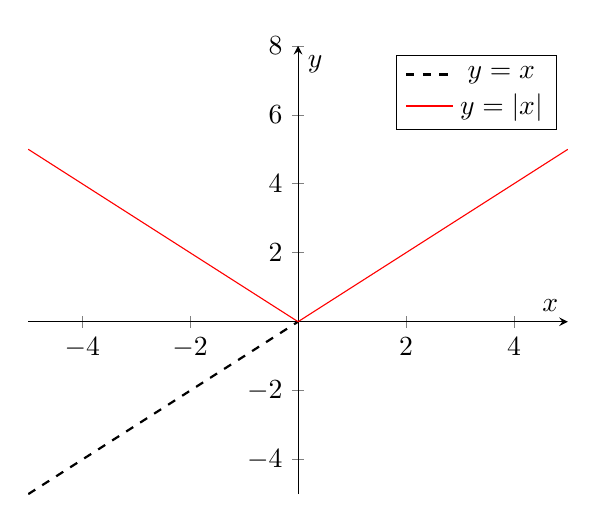
\begin{tikzpicture}
\begin{axis}[
    axis lines = middle,
    xlabel = $x$,
    ylabel = $y$,
    xmin=-5, xmax=5,
    ymin=-5, ymax=8,
   % width=\textwidth,
    %height=10cm,
]
\addplot[black, dashed, thick, domain=-5:0, samples = 200] {x};
\addlegendentry{$y=x$}
\addplot[red, domain=-5:0, samples = 200] {-x};
\addplot[red, domain=0:5, samples = 200] {x};
\addlegendentry{$y=|x|$}
\end{axis}
\end{tikzpicture}
\end{center}

\end{example}

Da wir uns nun mit Funktionen auskennen, können wir in ein zentrales Themengebiet der Analysis übergehen: die Differentialrechnung.

\newpage


\subsection{Grundlagen der Differentialrechnung}


\begin{definition} \textbf{(Über das Schneiden und Berühren zweier Graphen)} 
\begin{enumerate}
\item Die Graphen zweier Funktionen $f$ und $g$ schneiden\index{Funktion!Schneiden und Berühren} \index{Schneiden zweier Funktionen} sich in einem Punkt genau dann, wenn sie diesen Punkt gemeinsam haben.
\item Die Graphen zweier Funktionen $f$ und $g$ berühren\index{Funktion!Berühren} sich in einem Punkt genau dann, wenn sie diesen Punkt gemeinsam und dort die gleiche Steigung haben.
\item Eine Gerade, die einen Funktionsgraphen in einem Punkt berührt, heißt \textbf{Tangente}. \index{Tangente}
\item Eine Gerade, die einen Funktionsgraphen in mehreren Punkten schneidet, heißt \textbf{Sekante}. \index{Sekante}
\end{enumerate}
\end{definition} 

\begin{definition} \textbf{(Formale Grundbegriffe der Ableitung)}
\begin{enumerate}
\item Der Term $\dfrac{f(x)-f(x_0)}{x-x_0}$ heißt \textbf{Differenzenquotient}.
\item Der Grenzwert $\lim\limits_{x\to x_0} \dfrac{f(x)-f(x_0)}{x-x_0} = \lim\limits_{h \to 0} \dfrac{f(x_0+h)-f(x_0)}{h}$ heißt \textbf{Differentialquotient}.
\item Eine Funktion $f$ heißt an der Stelle $x_0$ differenzierbar, wenn der beidseitige Grenzwert des Differenzenquotienten existiert und gleich ist.
\item Für eine an der Stelle $x_0$ differenzierbare Funktion heißt der Differentialquotient \[ f'(x_0)=\lim_{x\to x_0} \dfrac{f(x)-f(x_0)}{x-x_0} = \lim_{h \to 0} \dfrac{f(x_0+h)-f(x_0)}{h} \] \textbf{Ableitung von $\mathbf{f}$ an der Stelle $\mathbf{x_0}$}.
\end{enumerate}
\index{Differentialquotient} \index{Funktion!Ableitung} \index{Ableitung}
\end{definition}

\begin{example}
Betrachten wir die Funktion $f(x)=x^2$ an der Stelle $x_0=1$. Den Differentialquotienten bestimmen wir wiefolgt:
\[ \lim_{h\to 0^+} =  \dfrac{f(x_0+h)-f(x_0)}{h} = \lim_{h\to 0^+} \dfrac{(1+h)^2-1^2}{h} = \lim_{h\to 0^+} \dfrac{2h+h^2}{h} =  \lim_{h\to 0^+} 2+h = 2\]
\[ \lim_{h\to 0^-} =  \dfrac{f(x_0+h)-f(x_0)}{h} = \lim_{h\to 0^-} \dfrac{(1+h)^2-1^2}{h} = \lim_{h\to 0^-} \dfrac{2h+h^2}{h} =  \lim_{h\to 0^-} 2+h =2\]
Da der Grenzwert existiert und beidseitig übereinstimmt ($2=2$ ist offensichtlich), heißt $f$ für $x_0 = 1$ differenzierbar mit Ableitung $f'(1)=2$. \par
Graphisch können wir die Abeltiung auch ermitteln. Sie ist die Steigung der Tangente, die den Graphen $G_f$ im Punkt $P(x_0|f(x_0))$ berührt. Wir sehen:
\begin{center}
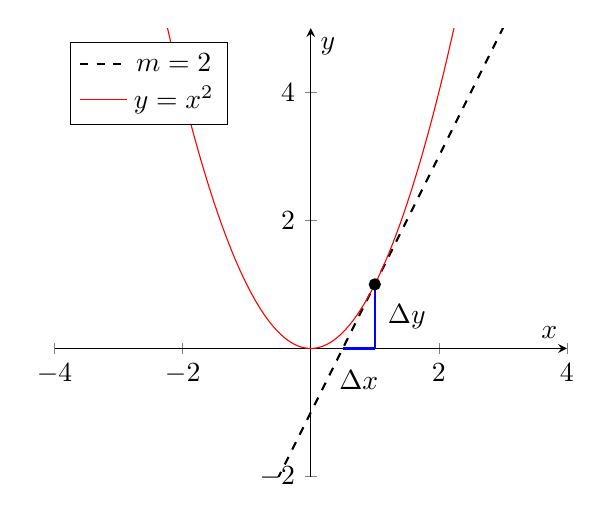
\begin{tikzpicture}
\begin{axis}[
    axis lines = middle,
    xlabel = $x$,
    ylabel = $y$,
    xmin=-4, xmax=4,
    ymin=-2, ymax=5,
    legend pos = north west,
    axis equal image
]

% Gerade y=x
\addplot[black, dashed, thick, domain=-4:4, samples=200] {2*x-1};
\addlegendentry{$m=2$}

% Parabel
\addplot[red, domain=-4:4, samples=200] {x^2};
\addlegendentry{$y=x^2$}

% Punkt (1,1)
\addplot[mark=*] coordinates {(1,1)};

% Steigungsdreieck für y = x
% horizontal
\addplot[blue, thick] coordinates {(1/2,0) (1,0)};
% vertikal
\addplot[blue, thick] coordinates {(1,0) (1,1)};
% Beschriftungen
\node at (axis cs:0.75,-0.5) {$\Delta x$};
\node at (axis cs:1.5,0.5) {$\Delta y$};

\end{axis}
\end{tikzpicture}
\end{center}
Durch das Ermiltten des Steigungsdreiecks ergibt sich $m=\dfrac{\Delta y}{\Delta x} = \dfrac{1}{\frac{1}{2}} = 2$
\end{example}

Im Folgenden ersetzen wir die Bezeichnung $f'(x_0)$ durch $f'(x)$ und meinen damit eine ganze Funktion, die Ableitungsfunktion:

\begin{definition} \textbf{(Ableitungsfunktion)} \par
Sei $f:D_f \rightarrow W_f, x \mapsto f(x)$ eine vollständig differenzierbare Funktion, so heißt die Funktion $f'(x)$ die \textbf{Ableitungsfunktion} von $f$, die jedem $x_0\in D_f$ die Steigung an der Stelle $x_0$ (Ableitung) zuordnet.
\end{definition}

\begin{theorem}\textbf{(Ableitungen ausgewählter Funktionen)} \par
\renewcommand{\arraystretch}{1.3}
\begin{tabularx}{\textwidth}{X | X}

\textbf{Funktion $f(x)$} & \textbf{Ableitung $f'(x)$} \\
\hline
Konstante Funktion \hfill $c=konst.$ & $0$ \\
\hline
Potenzfunktion \hfill $x^n$, $n\in\Q \setminus \{ 0 \}$ & $n\cdot x^{n-1}$ (Potenzregel) \\
\hline
Sinusfunktion \hfill $\sin x$ & $\cos x$ \\
\hline
Kosinusfunktion \hfill $\cos x$ & $-\sin x$ \\
\hline
Exponentialfunktion \hfill $a^x$ & $(\ln a)\cdot a^x$ \\
\hline
$e$-Funktion \hfill $e^x$ & $e^x$ \\
\hline
Logarithmusfunktion \hfill $\log_a x$ & $\frac{1}{(\ln a) x}$\\
\hline
$\ln$-Funktion \hfill $\ln x$ & $\frac{1}{x}$ \\
\end{tabularx}
\renewcommand{\arraystretch}{1}
\label{Satz:Ableitungen_Funktionen}
\end{theorem}

%\subsubsection{Ableitungsregeln}
Wir fassen hier die wichtigsten Ableitungsregeln zusammen, und gehen anschließend auf einige Beispiele ein.

\begin{theorem} \textbf{(Ableitungsregeln)} \par
Sei $k\in \R \setminus \{ 0 \}$ eine Konstante und $u(x), v(x)$ zwei vollständig differenzierbare Funktionen. Dann gilt:
\begin{enumerate}
\item $f(x)= k \cdot u(x) \Rightarrow f'(x)=k \cdot u'(x)$ (Faktorregel)
\item $f(x)=u(x)+v(x) \Rightarrow f'(x)=u'(x)+v'(x)$ (Summenregel)
\item $f(x)=u(x) \cdot v(x) \Rightarrow f'(x)=u'(x)\cdot v(x) + u(x)\cdot v'(x)$ (Produktregel)
\item $f(x)=\dfrac{u(x)}{v(x)} \Rightarrow f'(x)=\dfrac{u'(x)\cdot v(x) - u(x) \cdot v'(x)}{\mleft( v(x) \mright)^2}$ (Quotientenregel)
\item $f(x)=u(v(x)) \Rightarrow f'(x)=u'(v(x))\cdot v'(x)$ (Kettenregel)
\end{enumerate}
\textit{Bemerkung:} Die Regeln 1, 2, 3 und 5 stehen in der Formelsammlung. Die Quotientenregel ist äußerst praktisch, deshalb lohnt es sich, diese auswendig zu lernen.
\label{Satz:Ableitungsregeln}
\index{Ableitungsregeln} \index{Funktion!Ableitungsregeln} \index{Produktregel} \index{Quotientenregel} \index{Kettenregel}
\end{theorem}
 
Um die Sätze \ref{Satz:Ableitungen_Funktionen} und \ref{Satz:Ableitungsregeln} zu üben, folgen hier einige Beispiele:

\begin{example} \
\begin{enumerate}
\item $y=4x^3+x^2+ \sin x \Rightarrow y' = 12x^2+2x+\cos x$
\item $y=\cos x + \sin x \Rightarrow y' = - \sin x + \cos x$
\item $y=4 \sin x \Rightarrow y'=4 (\sin x)'=4\cos x$
\item $y=(4x^3-3x)\cdot (2e^x-\sin x) \Rightarrow y'=(12x^2-3)(2e^x-\sin x)+(4x^3-3x)(2e^x-\cos x)$
\item $y=\dfrac{\ln x}{e^x} \Rightarrow y'=\dfrac{1-\ln x}{x\cdot e^x}$
\item $y=(3x-4)^{2026} \Rightarrow y'=2026 \cdot (3x-4)^{2025} \cdot 3 = 6078 (3x-4)^{2025}$
\end{enumerate}
\end{example}

\newpage

\subsection{Anwendung der Differentialrechnung}
%\subsubsection{Bestimmung einer Tangente bzw. Normalen}
\begin{theorem}
Sei $f(x)$ eine vollständig differenzierbare Funktion. Dann erhalten wir die Tangentengleichung für einen Punkt $P(x_0|f(x_0))$ wiefolgt:

\begin{enumerate}
\item Bestimme den Term der Ableitung der Funktion $f(x)$.
\item Bestimme die Steigung an der Stelle $x_0$: $m=f'(x_0)$.
\item Bestimme den $y$-Wert $f(x_0)$. 
\item Setze alle Werte in die Tangentengleichung ein: $f(x_0)=f'(x_0) \cdot x_0 +t = m x_0 +t$
\item Bestimme zuletzt $t$ und gebe die vollständige Tangentengleichung an.
\end{enumerate}
Dieses Vorgehen ist analytisch und lässt sich leicht nachvollziehen. Eine andere Möglichkeit, die sich eher zum Auswendiglernen anbietet, und zu den oben genannten Schritten äquivalent ist, ist die Folgende: \par
\[ y=f'(x_0) \cdot (x-x_0)+f(x_0) \]
\label{Satz:Tangente}
\index{Tangente!Bestimmung der Tangentengleichung}
\end{theorem}

\begin{example}
Betrachten wir die Funktion $f(x)= x^3-4x+2$. Die Tangentengleichung für $x=2$ erhalten wir nach Methode \glqq unten\grqq \ durch
\[ y=f'(2) \cdot (x-2) + f(2) = 8 (x-2) + 2 = 8x -14  \]
Es ist eine gute Übung, die fünf Schritte durchzugehen, um die obere Rechnung nachzuvollziehen und die Tangente für $x=-1$ mit beiden Methoden zu bestimmen.
\label{Bsp:Tangente}
\end{example}

Neben der Tangente gibt es auch noch eine weitere Gerade, die manchmal eine Rolle spielt. Hierbei handelt es sich um die Normale.

\begin{definition}
Eine Gerade heißt Normale, wenn sie einen Graphen im $\ang{90}$-Winkel schneidet.
\end{definition}

\begin{theorem}
Sei $P(x_0|f(x_0))$ ein Punkt eines Graphen $G_f$ von einer vollständig differenzierbaren Funktion $f$, so ist die Gleichung
\[ y=\frac{-1}{f'(x_0)}\cdot (x-x_0) + f(x_0)\]
die Gleichung der Normalen durch den Punkt $P$.
\label{Satz:Normale}
\index{Normale}
\end{theorem}

\begin{example}
Greifen wir nochmals die Funktion aus Beispiel \ref{Bsp:Tangente} auf. Mithilfe der Formel aus Satz \ref{Satz:Normale} erhalten wir die Normalengleichung
\[ y=\dfrac{-1}{8}(x-2)+2  \]
Zusammen mit der Tangentengleichung erhalten wir folgendes Bild:
\begin{center}
\begin{tikzpicture}
\begin{axis}[
    axis lines = middle,
    xlabel = $x$,
    ylabel = $y$,
    xmin=-6, xmax=6,
    ymin=-3, ymax=6,
    legend pos = north west,
    axis equal image,
    width=\textwidth
]


%\addplot[black, dashed, thick, domain=-4:4, samples=200] {x^3-4*x+2};
%\addlegendentry{$m=2$}

% Parabel
\addplot[black, domain=-3:3, samples=200] {x^3-4*x+2};
\addlegendentry{$y=x^3-4x+2$}

%Tangente
\addplot[red, dashed, domain=-6:6, samples=200] {8*x-14};
\addlegendentry{Tangente}

%Normale
\addplot[blue, dashed, domain=-6:6, samples=200] {(-1/8)*x+2.25};
\addlegendentry{Normale}

% Punkt (2,2)
\addplot[mark=*] coordinates {(2,2)};

\end{axis}
\end{tikzpicture}
\end{center}
Hier bietet es sich an, die Schritte aus Satz \ref{Satz:Tangente} auf die Normale zu übertragen und zu überlegen, welche Schritte gleich, und welche unterschiedlich sind.
\end{example}

%\subsubsection{Monotonie und Krümmungsverhalten}

Das Monotonie- und Krümmungsverhalten einer (zweimal differenzierbaren) Funktion $f(x)$ kann man im wesentlichen über die erste und zweite Ableitung $f'(x)$ und $f''(x)$ bestimmen.
\paragraph{Geometrische Bedeutung der ersten Ableitung} Die erste Ableitung repräsentiert anschaulich die Steigung des Graphen an der betrachteten Stelle. Für eine Stelle $x_0$ gilt nun:
\begin{itemize}
\item $f'(x_0)>0$: Der Funktionsgraph wächst \textit{streng monoton}.
\item $f'(x_0)=0$: Der Funktionsgraph hat die Steigung $0$ und verläuft an dieser Stelle flach.
\item $f'(x_0)<0$: Der Funktionsgraph fällt \textit{streng monoton}.
\end{itemize}
\paragraph{Geometrische Bedeutung der zweiten Ableitung} Die zweite Ableitung beschreibt \glqq die Steigung der Steigung\grqq. Viel anschaulicher ist aber die Formulierung, dass die zweite Ableitung die Änderung des Monotonieverhaltens ist, also angibt, wie viel sich die Steigung an der Stelle $x_0$ ändert. Man spricht hierbei auch vom \textbf{Krümmungsverhalten}. Es gilt:

\begin{itemize}
\item $f''(x_0)>0$: Die \textit{Steigung} des Graphen $G_f$ nimmt an der Stelle $x_0$ zu, d.h. die Tangente \textit{dreht sich im Uhrzeigersinn}. Der Graph $G_f$ besitzt daher an der Stelle $x_0$ eine \textbf{Linkskrümmung}.
\item $f''(x_0)<0$: Die \textit{Steigung} des Graphen $G_f$ nimmt an der Stelle $x_0$ ab, d.h. die Tangente \textit{dreht sich gegen den Uhrzeigersinn}. Der Graph $G_f$ besitzt daher an der Stelle $x_0$ eine \textbf{Rechtskrümmung}.
\end{itemize}
Wir fassen diese Erkenntnisse im nächsten Satz zusammen:

\begin{theorem}
Sei $f(x)$ eine zweimal differenzierbare Funktion. Betrachtet man die erste Ableitung $f'(x_0)$ an der Stelle $x_0$, so gilt:
\begin{itemize}
\item $f'(x_0)>0 \Rightarrow$ Die Funktion \textit{wächst} an der Stelle \textit{streng monoton}.
\item $f'(x_0)<0 \Rightarrow$ Die Funktion \textit{fällt} an der Stelle \textit{streng monoton}.
\item $f'(x_0)=0 \Rightarrow$ Die Funktion verläuft an der Stelle flach.
\end{itemize}
Für die zweite Ableitung $f''(x_0)$ gilt:
\begin{itemize}
\item $f''(x_0)>0 \Rightarrow$ Die Funktion ist an der Stelle \textit{linksgekrümmt}.
\item $f''(x_0)<0 \Rightarrow$ Die Funktion ist an der Stelle \textit{rechtsgekrümmt}.
\end{itemize}
\label{Satz:KrümmungMonotonie}
\index{Funktion!Krümmung}
\index{Funktion!Monotonie}
\index{Krümmungsverhalten einer Funktion}
\index{Monotonie einer Funktion}
\end{theorem}

\begin{example}
\item Betrachten wir zuerst die Normalparabel $y=x^2$. Für die erste Ableitung gilt: $y'=2x$. Deshalb können wir das Monotonieverhalten aufteilen in das Intervall $]-\infty, 0[$, indem die Funktion streng monoton fallend ist ($y'<0$). Für $x=0$ gilt $y'=0$, also ist hat die Normalparabel dort eine \glqq flache\grqq \ Stelle, an der der Graph waagrecht verläuft. Für $x>0$ ist die Normalparabel streng monoton steigend. Nun ermitteln wir die zweite Ableitung: $y''=2$. Deshalb ist die Normalparabel überall linksgekrümmt.
\begin{center}
\begin{tikzpicture}
\begin{axis}[
    axis lines = middle,
    xlabel = $x$,
    ylabel = $y$,
    xmin=-5, xmax=5,
    ymin=-2, ymax=5,
    legend pos = north west,
    axis equal image,
    width=\textwidth
]


%\addplot[black, dashed, thick, domain=-4:4, samples=200] {x^3-4*x+2};
%\addlegendentry{$m=2$}

% Parabel
\addplot[blue, domain=-3:3, samples=200] {x^2};
\addlegendentry{$y=x^2$}

% 1. Ableitung
\addplot[red, domain=-3:3, samples=200] {2*x};
\addlegendentry{$y'=2x$}

% 2. Ableitung
\addplot[black, domain=-5:5, samples=200] {2};
\addlegendentry{$y''=2$}

\end{axis}
\end{tikzpicture}
\end{center}
\label{Bsp:Monotonie}
\end{example}

%\subsubsection{Extrem- Wende- und Terassenpunkte}

\begin{definition} \textbf{(Extrem-, Wende- und Terassenpunkte)} \par
Sei $f(x)$ eine dreifach differenzierbare Funktion. Dann heißt für
\begin{enumerate}
\index{Extrempunkt}
\item $f'(x_0)=0, f''(x_0)> 0$ der Punkt $P(x_0|f(x_0))$ \textbf{Tiefpunkt}, \index{Tiefpunkt}
\item $f'(x_0)=0, f''(x_0)< 0$ der Punkt $P(x_0|f(x_0))$ \textbf{Hochpunkt}, \index{Hochpunkt}
\item $f'(x_0)=0, f''(x_0)= 0, f'''(x_0)\neq 0$ der Punkt $P(x_0|f(x_0))$ \textbf{Terassenpunkt} oder Sattelpunkt, \index{Terassenpunkt} \index{Sattelpunkt}
\item $f''(x_0)= 0, f'''(x_0)\neq 0$ der Punkt $P(x_0|f(x_0))$ \textbf{Wendepunkt}. \index{Wendepunkt}
\end{enumerate}
Tief- und Hochpunkte werden oft auch gemeinsam als \textbf{Extrempunkte} bezeichnet, nimmt man Terassenpunkte hinzu, so spricht man von \textbf{kritischen Punkten}.
\label{Def:Extrempunkte}
\end{definition}
Aus der Definition ergibt sich unmittelbar, dass jeder Terassenpunkt ein Wendepunkt, aber nicht jeder Wendepunkt ein Terassenpunkt ist. Bei Terassen- und insbesondere Wendepunkten wird häufig noch danach gefragt, ob von links- nach rechtsgekrümmt oder der Graph andersherum sein Krümmungsverhalten ändert. \par
Alternativ zur Betrachtung der zweiten Ableitung kann man auch eine Vorzeichentabelle machen. Dabei setzt man Werte nahe der zu untersuchenden Stelle ein und überprüft, ob sie positiv oder negativ sind. Es gilt:
\begin{theorem} \textbf{(Kriterien für kritische Punkte)}
\begin{enumerate}
\item \textbf{Tiefpunkt:} $f'(x_0)=0, f''(x_0)>0$ \textit{oder} $f'(x_0)=0$ und Vorzeichenwechsel bei $x_0$ von $- \to +$.
\item \textbf{Hochpunkt:} $f'(x_0)=0, f''(x_0)<0$ \textit{oder} $f'(x_0)=0$ und Vorzeichenwechsel bei $x_0$ von $+ \to -$.
\item \textbf{Terassenpunkt:} $f'(x_0)=0, f''(x_0)=0, f'''(x_0)\neq 0$ \textit{oder} $f'(x_0)=0$ und kein Vorzeichenwechsel an der Stelle $x_0$.
\end{enumerate}
Für die oben genannten Punkte sind beide Aussagen äquivalent. Es ist insbesondere egal, ob man eine Vorzeichentabelle oder die nächsthöhere Ableitung ermittelt.
\index{Vorzeichentabelle}

\end{theorem}
Betrachte nun erneut Beispiel \ref{Bsp:Monotonie}, und versuche, die \glqq flache Stelle\grqq \ mithilfe der Fachsprache aus der Definition \ref{Def:Extrempunkte} genauer zu beschreiben. Ein anderes Beispiel liefert vielleicht noch mehr Klarheit:

\begin{example} \
\begin{enumerate}
\item Sei $f(x)=\frac{1}{3}x^3-4x$ die betrachtete Funktion und unsere Aufgabe, die Wende- und Extrempunkte zu bestimmen. Zuerst bestimmen wir dafür die ersten drei Ableitungen:
\[ f'(x)=x^2-4,\hspace{1cm} f''(x)=2x, \hspace{1cm} f'''(x)=2\]
Für Extrempunkte gilt es, die Nullstellen der ersten Ableitung herauszufinden. Diese liegen bei $x_0=\pm 2$. Weil für $f''(x_0) = \pm 4 \neq 0$ gilt, liegen hier jeweils Extrempunkte vor. Für $x_0=-2$ ist die zweite Ableitung negativ. Also hat $f$ hier einen Hochpunkt. Analog gilt, dass $f$ bei $x_0=+2$ einen Tiefpunkt hat. Für den Wendepunkt bestimmen wir die Nullstellen der zweiten Ableitung und erhalten $x_W=0$. Da die dritte Ableitung für diesen $x$-Wert positiv ist, handelt es sich um einen Übergang von rechtsgekrümmt nach linksgekrümmt. Mithilfe der Funktionswerte geben wir nun die wirklichen Punkte an: \\
\[ H(-2|f(-2)) = (-2|\frac{16}{3}) \hspace{1cm} T(2|f(2)) = (2|\frac{-16}{3}) \hspace{1cm} W(0|f(0)) = (0|0)  \]
\begin{center}
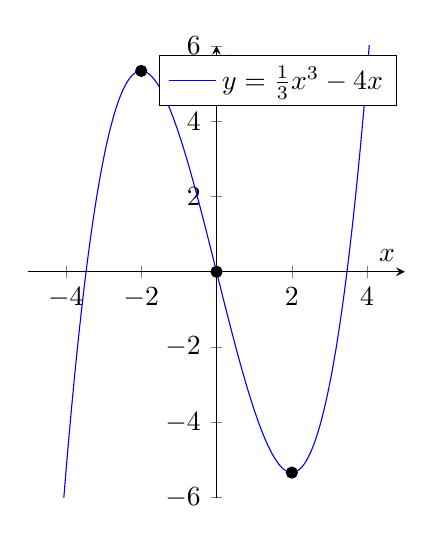
\begin{tikzpicture}
\begin{axis}[
    axis lines = middle,
    xlabel = $x$,
    ylabel = $y$,
    xmin=-5, xmax=5,
    ymin=-6, ymax=6,
    %legend pos = north west,
    axis equal image,
    width=0.7\textwidth
]


%\addplot[black, dashed, thick, domain=-4:4, samples=200] {x^3-4*x+2};
%\addlegendentry{$m=2$}

% Parabel
\addplot[blue, domain=-5:5, samples=200] {(1/3)*x^3-4*x};
\addlegendentry{$y=\frac{1}{3}x^3-4x$}

\addplot[mark=*] coordinates {(0,0)};
\addplot[mark=*] coordinates {(-2,16/3)};
\addplot[mark=*] coordinates {(2,-16/3)};

\end{axis}
\end{tikzpicture}
\end{center}
\item Durch Nachrechnen findet man heraus, dass die Funktion $y=(x-3)^3+5$ bei $T(3|5)$ einen Terassenpunkt hat. (Übung)
\end{enumerate}
\end{example}

%\subsubsection{Zusammenfassung bis hierhin: Kurvendiskussion}
Aufbauend auf den vorherigen Kapiteln können wir nun intensive Betrachtungen für Funktionen und deren Verlauf anstellen. Bei dem Begriff \textit{Kurvendiskussion} geht es um die \textit{Untersuchung und Feststellung der Funktionseigenschaften und des Funktionsverlaufs}. Es gibt dabei kein konkretes Schema, aber häufig sind die folgenden Aspekte gefordert. Deshalb empfehle ich, diese Aspekte gut zu üben, um eine gute Prüfungsvorbereitung zu gewährleisten.
\begin{itemize}
\item Bestimmung des Definitionsbereiches (Definitionslücken)
\item Symmetrie (Punktsymmetrisch? Achsensymmetrisch?)
\item Null\textbf{stellen}, Schnitt\textbf{punkte} mit der $y$-Achse
\item (Senkrechte) Asymptoten
\item Ableitungen (i.d.R. bis zur dritten Ableitung)
\item Bestimmung der Extremwerte (Minima, Maxima)
\item Wendepunkte, Sattelpunkte
\item Verhalten der Funktion für $x\rightarrow \pm \infty$, Asymptoten im Unendlichen (waagrecht oder schräg)
\item Wertemenge der Funktion
\item Zeichnen der Funktion (sowie der Ableitung, und der Stammfunktion)
\item Untersuchung des Krümmungsverhaltens
\item Monotonie
\end{itemize}


%\subsubsection{Extremwertaufgaben}
Ein etwas anderes Aufgabengebiet, und auch nicht wirklich der Analysis zuzurechnen, stellt der Bereich der Extremwertaufgaben da. Denn eigentlich geht es nicht, wie sonst bei der Analysis, um Funktionen, sondern um Gleichungen, die wir auflösen. Jedoch können wir mit unserem Wissen dieses Aufgabenformat, das wir seit der Mittelstufe kennen, etwas einfacher bearbeiten. \par
Zuerst stellt man in solchen Aufgabenformaten typischerweise die \textbf{Hauptbedingung} auf, eine Funktionsgleichung, die als Ergebnis die zu optimierende Größe liefert. Dabei kommt meist mehr als eine Variable vor. Anschließend stellt man eine Beziehung (die \textbf{Nebenbedingung}) zwischen Variablen auf und stellt diese Beziehung nach einer beliebigen Variable um. Bei drei Variablen sind zwei Nebenbedingungen erforderlich, usw. Hat man keine Idee, woraus man die Nebenbedingung(en) erstellen kann, so schaut man nochmal in der Aufgabenstellung nach mit der Frage im Kopf, welche Bedingung man noch nicht genutzt hat. Nun wird die Neben- in die Hauptbedingung eingesetzt. Dabei erhält man eine Funktion mit nur einer Variablen. Nun kann man die Funktion nach der Variablen ableiten und die Untersuchung als Extremwert-Problem betrachten (also Extrempunkte bestimmen). Die restlichen Größen werden laut Aufgabenstellung bestimmt. (\textit{Achtung: In der Praxis werden hier gerne Punkte liegengelassen, weil man diesen Aufgabenteil übersieht.}) Wir fassen diese Schritte im nächsten Satz zusammen:
\begin{theorem}\textbf{(Lösen von Extremwertaufgaben)}
\begin{enumerate}
\item Stelle eine Funktionsgleichung auf, die als Ergebnis die zu optimierende Größe liefert. \textbf{(Hauptbedingung)}
\item Stelle Beziehungen zwischen den Variablen auf. \textbf{(Nebenbedingungen)}
\item Setze die Nebenbedingungen in die Hauptbedingung ein.
\item Ermittle den gesuchten Extremwert (Hoch- oder Tiefpunkt).
\item Bestimme die restlichen Größen.
\end{enumerate}
\label{Satz:Extremwertaufgaben}
\index{Extremwertaufgaben}
\end{theorem}

\begin{example}
Ein Schäfer will mit $\SI{100}{\meter}$ Maschendraht für einen Zaun ein rechteckiges Feld für seine Schafe begrenzen, sodass die Fläche darin möglichst groß wird. Welche Länge $l$ und Breite $b$ muss das Rechteck erhalten?\par
Wir befolgen das Lösungsschema aus Satz \ref{Satz:Extremwertaufgaben}:
\begin{enumerate}
\item Die zu optimierende Größe ist der Flächeninhalt. Für ein Rechteck gilt: 
\[ A=l\cdot b \]
\item Die Gesamtlänge des Zaunes entspricht dem Umfang. Für ihn gilt:
\[ 2l + 2b = \SI{100}{\meter}	\Leftrightarrow 2l = \SI{100}{\meter} - 2b \Leftrightarrow l = \SI{50}{\meter}	- b \]
\item Wir setzen die Nebenbedingung in die Hauptbedingung ein: 
\[ A= (\SI{50}{\meter} -b)\cdot b =  \SI{50}{\meter} \cdot b - b^2 \]
\item Wir wollen den \textit{maximalen} Flächeninhalt bestimmen, suchen also den Hochpunkt der Funktion, die den Flächeninhalt beschreibt.
\[ A(b)=  \SI{50}{\meter} \cdot b - b^2\]
\[ A'(b)= \SI{50}{\meter} - 2b \]
\[ 0 = \SI{50}{\meter} - 2b_E \]
\[ 2b_E = \SI{50}{\meter} \Rightarrow b_E = \SI{25}{\meter} \]
wobei $b_E$ der Wert für den Extrempunkt darstellt. Um sicher zu gehen, prüfen wir, ob es sich dabei tatsächlich um einen Extrempunkt handelt. Dafür muss die zweite Ableitung an dieser Stelle kleiner $0$ sein. Tatsächlich gilt $A''(25)=-2 < 0$. (Übung)
\item Nachdem wir die Breite bestimmt haben, suchen wir noch die Länge des Rechteckes. Indem wir in die Nebenbedingung aus Schritt 2. einsetzen erhalten wir: $l_E=\SI{25}{\meter}$. 
\end{enumerate}
Oft ist ein Abschlusssatz schön. Deshalb schließen wir die Aufgabe mit den Folgenden Worten: \par
Der Schäfer sollte ein Quadrat der Seitenlänge $\SI{25}{\meter}$ wählen, um den größtmöglichen Flächeninhalt mit den $\SI{100}{\meter}$ Zaun zu erhalten.
\end{example}

\newpage

\subsection{Integralrechnung}
Im Unterricht haben wir Integrale als gemeinsamen Grenzwert von Ober- und Untersummen kennengelernt. Auf eine Wiederholung davon gehe ich an dieser Stelle nicht mehr ein, denn diese Vorüberlegung ist für den weiteren Verlauf aus meiner Sicht zu unwichtig, um ausführlich behandelt zu werden. Es lohnt sich aber dennoch, falls man genügend Zeit und Motivation hat, diese Einführung nochmals anzusehen! \par
Im Schulbuch wird an dieser Stelle aber noch die Summenschreibweise wiederholt, die ich hier deshalb auch nochmal anreißen möchte:
\[ \sum_{i=1}^n s_i = s_1 + s_2 + s_3 + ... + s_{n-1} + s_n  \]
\index{Summensymbol}
\begin{definition}
Sei $f$ eine integrierbare Funktion, dann heißt jede Funktion $F(x)$ \textbf{Stammfunktion} von $f$, wenn gilt:
\[ F'(x)=f(x) \]
\index{Stammfunktion} \index{Funktion!Stammfunktion}
\end{definition}

\begin{example}
Gegeben ist die Funktion $f(x)=4x^3-8x$, so ist jede Funktion $F_c(x)=x^4-4x^2+c$ mit $c\in \R$ eine Stammfunktion, da die Ableitung der Funktion $F$ wieder $f$ ergibt. (Übung)
\begin{center}
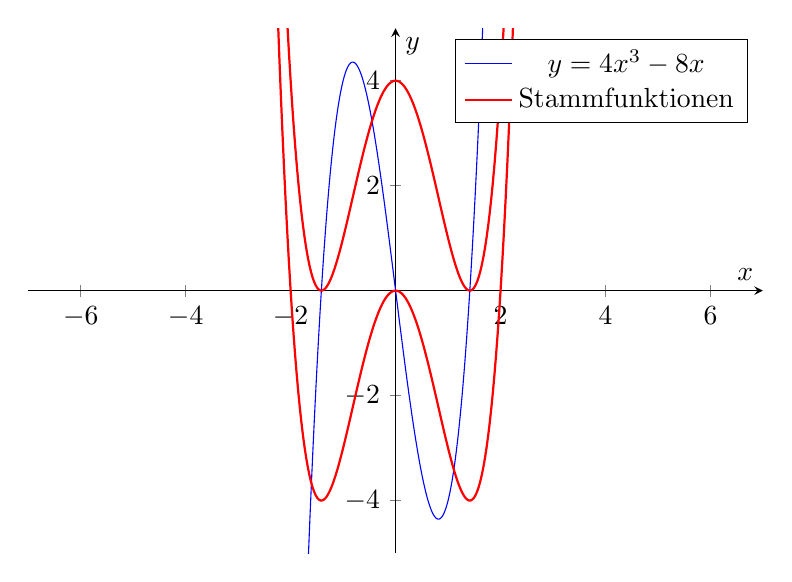
\begin{tikzpicture}
\begin{axis}[
    axis lines = middle,
    xlabel = $x$,
    ylabel = $y$,
    xmin=-7, xmax=7,
    ymin=-5, ymax=5,
    %legend pos = north west,
    axis equal image,
    width=0.9\textwidth
]



% Parabel
\addplot[blue, domain=-2:2, samples=200] {4*x^3 - 8*x};
\addlegendentry{$y=4x^3-8x$}

\addplot[red, thick, domain=-3:3, samples=200] {x^4-4*x^2+4};
\addplot[red, thick, domain=-3:3, samples=200] {x^4-4*x^2};
\addlegendentry{Stammfunktionen}

\end{axis}
\end{tikzpicture}
\end{center}


\end{example}
%\subsubsection{Das bestimmte Integral}

\begin{definition} \textbf{(Bestimmtes Integral)} \par
Eine Funktion sei in einem Intervall $[a,b]$ definiert. Existiert der gemeinsame Grenzwert 
\[ \lim_{n\rightarrow +\infty} U_n = \lim_{n\rightarrow +\infty} O_n\] 
von Ober- und Untersumme im Intervall $[a,b]$, so nennt man diesen Grenzwert \textbf{bestimmtes Integral der Funktion $\mathbf{f}$} über $[a,b]$ und schreibt 
\[ \int_a^b f(x) \diff x  \]
Die Funktion $f$ nennt man dann \textbf{integrierbar} über $[a,b]$. Dabei heißt $f$ \textbf{Integrand} und die durch $\diff x$ gekennzeichnete Variable \textbf{Integrationsvariable}.
\index{Integral!Bestimmtes}
\index{Bestimmtes Integral}
\index{Integrand}
\end{definition}

\begin{theorem} \textbf{(Rechenregeln für das bestimmte Integral)} \par
\begin{enumerate}
\item $ \displaystyle \int_a^a f(x) \diff x = 0 $  
\item $\displaystyle \int_a^b f(x) \diff x + \int_b^c f(x) \diff x= \int_a^c f(x) \diff x $
\item $\displaystyle \int_b^a f(x) \diff x = -\int_a^b f(x) \diff x$
\end{enumerate}
\label{Satz:Rechenregeln_besIntegral}
\end{theorem}
Auf Beispiele wird an dieser Stelle verzichtet, die Rechenregeln werden in den folgenden Kapiteln aber Verwendung finden. \par
Im Abitur kann bzw. muss auch ohne Rechnung der Wert eines bestimmten Integrals ermittelt werden können. Es gibt dafür keine Allzweck-Methode, dennoch gibt es einige Ideen, mit denen man so eine Aufgabe bewältigen kann. 
\begin{enumerate}
\item \textbf{Kästchen zählen:} Das ist wohl die elementarste Variante. Zähle alle Kästchen unter dem Graphen bis zur $x$-Achse. Beachte immer den Maßstab: Wie groß ist ein Kästchen?
\item  \textbf{Geometrische Figuren:} Falls der Graph der Funktion gut liegt, kann es manchmal hilfreich sein, eine geometrische Figur, etwa ein Dreieck, Trapez, etc. in das Koordinatensystem zu zeichnen, das den Flächeninhalt möglichst gut approximiert (annähert). Die Formeln für diese elementargeometrischen Figuren sind Grundwissen und stehen zum Beispiel in der Formelsammlung. Für den hilfsmittelfreien Teil im Abitur ist es dennoch eine Überlegung wert, sich die Formeln auswendig zu merken.
\item Hast du weitere Ideen? Kreativ denken kann dir manchmal viel Zeit sparen. Wenn du also noch andere Ideen hast, ist das sehr gut!
\end{enumerate}

\begin{theorem}
Gegeben ist die auf dem Intervall $[a,b]$ integrierbare Funktion. Dann gibt das Integral $\displaystyle \int_a^b f(x) \diff x$ die \textbf{orientierte Flächenbilanz} der Fläche an, die der Graph von $f$ mit der $x$-Achse zwischen der unteren Grenze $a$ und der oberen Grenze $b$ einschließt. Dabei werden Flächeninhalte oberhalb der $x$-Achse positiv, darunterliegend negativ, gezählt.
\index{Flächenbilanz}
\end{theorem}
Man kann zeigen, dass für punktsymmetrische Funktionen zum Ursprung bzw.\ achsensymmetrische Funktionen zur y-Achse spezielle Rechenregeln gelten. Diese führen wir im nächsten Satz aus:

\begin{theorem}
Sei $f:x\mapsto f(x)$ eine auf dem Intervall $[-a,a]$ integrierbare Funktion und sei $a>0$. Dann gilt:
\begin{enumerate}
\item Falls $f$ punktsymmetrisch zum Ursprung ist, gilt \[ \displaystyle \int_{-a}^a f(x) \diff x = 0,\]
\item Falls $f$ achsensymmetrisch zur y-Achse ist, gilt \[ \displaystyle \int_{-a}^a f(x) \diff x = 2\cdot \int_{0}^a f(x) \diff x = 2\cdot \int_{-a}^0 f(x) \diff x.\]
\end{enumerate}
\label{Satz:Symmetrie_Integral}
\end{theorem}

Diese Erkenntnisse betrachten wir anhand des folgenden Beispiels:

\begin{example} \
\begin{enumerate}
\item Betrachten wir zuerst eine achsensymmetrische Funktion $y=x^2-4$. Blicken wir genauer auf den Intervall $[-2,2]$, so können wir diese orientierte Flächenbilanz schreiben als $\displaystyle \int_{-2}^2(x^2-4) \diff x$, wobei $(x^2-4)$ der Integrand ist und $x$ die Intergrationsvariable heißt.
\begin{center}
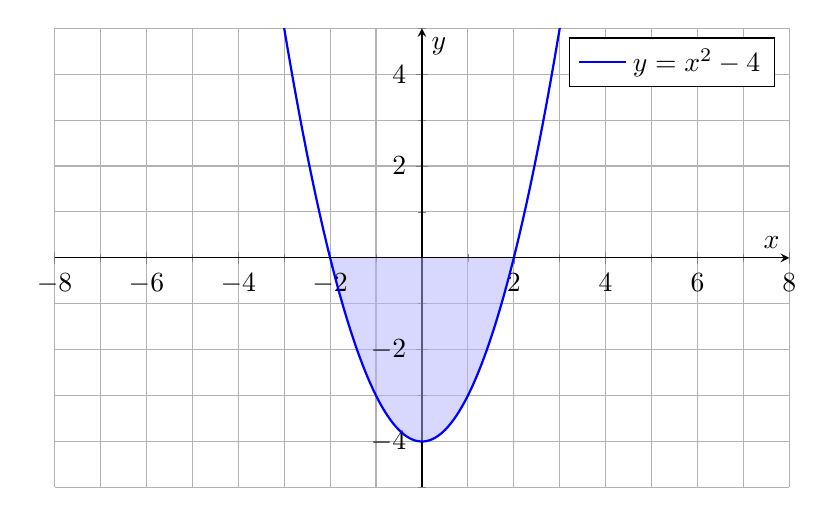
\begin{tikzpicture}
\begin{axis}[
    axis lines = middle,
    xlabel = $x$,
    ylabel = $y$,
    xmin=-8, xmax=8,
    ymin=-5, ymax=5,
    axis equal image,
    width=0.9\textwidth,
    grid=both,
    minor tick num=1,
    major grid style={gray!60},
    minor grid style={gray!60}
]

% Funktion
\addplot[name path=f, blue, thick, domain=-6:6, samples=200] {x^2-4};
\addlegendentry{$y=x^2-4$}

% x-Achse als zweite Kurve
\addplot[name path=xaxis, domain=-2:2] {0};

% Fläche zwischen Funktion und x-Achse
\addplot[
    blue!30,
    opacity=0.5
] fill between[
    of=f and xaxis,
    soft clip={domain=-2:2},
];

\end{axis}
\end{tikzpicture}
\end{center}
Durch Kästchenzählen kommen wir auf einen Wert zwischen $\num{10,5}$ und $11$. Wie wir später noch berechnen werden, ist der Betrag exakt $\frac{32}{3}\approx \num{10,67}$, wobei wir im Folgenden mit der ganzen Zahl $11$ arbeiten möchten. Bei der rein graphischen Bestimmung sind andere Werte natürlich auch denkbar. Jedenfalls stellen wir fest, dass die Fläche offenbar unter der x-Achse liegt. Deshalb muss die orientierte Flächenbilanz von $-2$ bis $2$ negativ sein. Wir schreiben deshalb:
\[ \int_{-2}^2 (x^2-4) \diff x \approx - 11 \]
Nun können wir auch die andere Richtung betrachten, also von $2$ bis $-2$ integrieren. Dabei erhalten wir nach Satz \ref{Satz:Rechenregeln_besIntegral} 3. genau das $(-1)$-fache:
\[ \int_{2}^{-2} (x^2-4) \diff x \approx 11 \]
Nach demselben Satz können wir auch Teilintervalle addieren, beispielsweise also 
\[ \int_{-2}^0 (x^2-4) \diff x + \int_{0}^2 (x^2-4) \diff x \approx -11\]
Es ist eine gute Übung, das nachzurechnen. Nun wissen wir, dass die Funktion achsensymmetrisch ist. Denn es gilt: $f(-x)=(-x)^2-4=x^2-4=f(x)$. Es genügt nach Satz \ref{Satz:Symmetrie_Integral} 2. also, sich das Integral von $0$ bis $2$ zu betrachten und mit Faktor $2$ zu multiplizieren. Durch Nachrechnen ergibt sich hier:
\[ \int_{-2}^2 (x^2-4) \diff x = 2\cdot \int_{0}^2 (x^2-4) \diff x \approx 2 \cdot \num{5,5} = 11\]
Für die nachfolgenden Kapitel sind diese Rechenregeln sehr praktisch, wenn wir analytisch den Flächeninhalt oder die orientierte Flächenbilanz bestimmen möchten. Für das Arbeiten am Graphen sind die Regeln noch nicht so praktisch.
\item Für die punktsymmetrische Funktion $y=x^3$ ist es eine gute Übung, den Graphen zu zeichnen und die orientierte Flächenbilanz in den Intervallen $[-1,1], [0,1], [-1,0], [-2,2], [2,-1]$ zu bestimmen. Dafür bietet es sich insbesondere an, die Methode des Kästchenzählens mit dem Einzeichnen von Dreiecken zu vergleichen.
\end{enumerate}
\label{Bsp:BesIntegral}
\end{example}

Da das Bestimmen von bestimmten Integralen mühselig sein kann und es vorkommt, dass man zu einer unteren Grenze in Abhängigkeit von $x$ die Flächenbilanz angeben soll, wurde der Begriff der Integralfunktion eingeführt. 

\begin{definition}
Sei $f$ eine im Intervall $I$ integrierbare Funktion $f:t\mapsto f(t)$. Dann heißt für jedes $a\in I$ die Funktion 
\[ I_a:x\mapsto \int_a^xf(t)\diff t  \]
mit $x\in I$ die \textbf{Integralfunktion von f zur unteren Grenze a}.
\index{Funktion!Integralfunktion} \index{Integral!funktion}
\end{definition}

\begin{theorem} \textbf{(Integralfunktion und Stammfunktion)} \par
Sei $f(x)$ eine auf dem Intervall $I$ integrierbare Funktion, $F(x)$ eine Stammfunktion und $I(x)$ eine Integralfunktion von $f$.
\begin{enumerate}
\item Eine Stammfunktion ist \textbf{genau dann} eine Integralfunktion zur unteren Grenze $a\in I$, wenn gilt: $F(a)=0$, also wenn die Stammfunktion an der Stelle $x=a$ eine Nullstelle hat.
\item Für die untere Grenze $a$ gilt: $\displaystyle I_a(a)=\int_a^af(t)\diff t = 0$.
\end{enumerate}
\label{Satz:Integralfunktion}
\end{theorem}

Der nun folgende Satz ist in der Mathematik ein sehr wichtiger. Er verbindet die uns bekannte Differentialrechnung, also das Ableiten, mit der Integralrechnung, dem Aufleiten! Weil dieser Satz so wichtig ist, heißt er auch so:

\begin{theorem} \textbf{(Hauptsatz der Differential- und Integralrechnung)} \par
Sei $f$ eine im Intervall $I$ stetige Funktion. Dann gilt für die Integralfunktion $\displaystyle I_a:x\mapsto \int_a^xf(t)\diff t$:
\[ I'_a(x)=f(x) \ \text{für} \ a,x \in I \]
In Worten: Jede Integralfunktion $I_a$ von $f$ ist eine Stammfunktion von $f$. 
\label{Satz:HDI}
\index{Hauptsatz der Differential- und Integralrechnung}
\end{theorem}

Das Folgende Bild fasst diese Erkenntnis nochmal zusammen: Jede Integralfunktion ist eine Stammfunktion, aber nicht jede Stammfunktion ist eine Integralfunktion. Das Kriterium, wann eine Stammfunktion eine Integralfunktion ist, wurde in Satz \ref{Satz:Integralfunktion} genannt.

\begin{center}
\begin{tikzpicture}

% Große Ellipse – Stammfunktionen
\draw[thick, fill=definitionblue!10] (0,0) ellipse (5cm and 3cm);
\node at (0,1) {Menge aller Stammfunktionen von $f$};

% Kleine Ellipse – Integralfunktionen
\draw[thick, fill=theoremred!15] (1,-1) ellipse (2.5cm and 1.2cm);
\node[text width=3 cm, align = center] at (1,-1) {Menge aller Integralfunktionen von $f$};

\end{tikzpicture}
\end{center}

\begin{example}
Eine einfache Überlegung stellt die Betrachtung der folgenden Funktion dar: $F_0(x)=\dfrac{1}{2}x^2$ ist eine Stammfunktion von $f(x)=x$, denn $F_0'(x)=\dfrac{1}{2}\cdot 2 \cdot x = x$. Auch ist $F_0$ eine Integralfunktion, denn sie besitzt an der Stelle $x=0$ eine Nullstelle. \par
Auch die Funktion $F_2(x)=\dfrac{1}{2}x^2+2$ ist eine Stammfunktion, denn die Konstante fällt beim Ableiten weg. Sie ist jedoch \textbf{keine} Integralfunktion, da sie keine Nullstelle besitzt!
\end{example}
Die Notation im obigen Beispiel impliziert bereits, dass wir für beliebige Konstanten eine Stammfunktion erzeugen können. Bevor wir diese Erkenntnis festhalten, schauen wir zuvor noch, wie wir rechnerisch und damit präzise den Flächeninhalt/die orientierte Flächenbilanz bestimmen können. 

\begin{theorem} \textbf{(Berechnung von Integralen)} \par
Sei $f$ eine im Intervall $[a,b]$ stetige Funktion und $F$ eine beliebige Stammfunktion in diesem Intervall. Dann gilt:
\[ \int_a^bf(x)\diff x = F(b)-F(a)  \]

\index{Integral!Berechnung des bestimmten} \index{Berechnung von Integralen}
\end{theorem}
Beim Berechnen der bestimmten Integrale nutzt man auch die Schreibweise
\[ \int_a^bf(x)\diff x = [F(x)]_a^b, \]
um kompakter zu formulieren. 

\begin{example}
Wir möchten nun mithilfe des Hauptsatzes der Differential- und Integralrechnung erste Intervalle berechnen und greifen dafür Beispiel \ref{Bsp:BesIntegral} auf. Dabei hatten wir die Funktion $f(x)=(x^2-4)$ betrachtet, und uns dann gefragt, wie groß die Flächenbilanz von $-2$ bis $2$ ist. Nun können wir das Ergebnis nachrechnen, indem wir eine Stammfunktion suchen: \par
$F(x)=\dfrac{1}{3}x^3-4x$ ist eine Stammfunktion, denn $F'(x)=x^2-4$. Also berechnen wir:
\[ \int_{-2}^2 (x^2-4) \diff x = \mleft[\dfrac{1}{3}x^3-4x\mright]_{-2}^2 = \dfrac{8}{3}-8 - \mleft( - \dfrac{8}{3} - (-8) \mright) = -\dfrac{32}{3} \approx -\num{10,67} \]
Unsere geometrische Näherung war also relativ gut, und nun haben eine Methode, das nachzurechnen. Für die punktsymmetrische Funktion aus Beispiel \ref{Bsp:BesIntegral} können die geometrischen Ergebnisse mittels des Hauptsatzes der Differential- und Integralrechnung nachgerechnet werden.
\end{example}

%\subsubsection{Das unbestimmte Integral}
Nachdem wir uns mit dem bestimmten Integral ausgiebig beschäftigt haben, folgt offensichtlich die Frage, wie wir Stammfunktionen überhaupt bestimmen wollen. Diese Frage hängt unmittelbar mit dem \textbf{unbestimmten Integral} zusammen. 

\begin{definition}
Sei $f$ eine integrierbare Funktion. Dann heißt die Menge aller Stammfunktionen \textbf{unbestimmtes Integral} von $f$. Man schreibt:
\[ \int f(x) \diff x = F(x)+c, \ c \in \R \]
In Worten: \glqq Integral f von x dx\grqq
\index{Unbestimmtes Integral} \index{Integral!Unbestimmtes}
\end{definition}
In manchen Aufgaben muss man \textit{eine} Stammfunktion angeben, hier genügt also explizit ein Beispiel. Ein häufiger Fehler ist das Vergessen der Konstante $+c$, wenn man das unbestimmte Integral bestimmen muss. Nun wenden wir uns ganz konkreten Regeln zu, die beim Integrieren gelten.

\begin{theorem} \
\begin{enumerate}
\item Sind $G$ und $H$ jeweils Stammfunktionen von $g$ und $h$, so gilt für alle $k\in \R$:
\begin{enumerate}[i)]
	\item $f:x \mapsto k \cdot g(x) \Rightarrow F:x\mapsto k \cdot G(x)$ und
	\item $f:x\mapsto g(x)+h(x) \Rightarrow F:x \mapsto G(x)+H(x)$, 
\end{enumerate}
wobei $F$ dabei eine mögliche Stammfunktion von $f$ ist.
\item Sind $f$ und $g$ zwei auf dem Intervall $I$ definierte Funktionen, so gilt für $k\in \R$ und $a,b \in I$:
	\begin{enumerate}[i)]
	\item $\displaystyle \int_a^b k\cdot f(x) \diff x = k \cdot \int_a^bf(x) \diff x$ und
	\item $\displaystyle \int_a^b(f(x)+g(x))\diff x = \int_a^bf(x)\diff x + \int_a^b g(x) \diff x$.
	\end{enumerate}
\end{enumerate}
\label{Satz:Int_Regeln}
\end{theorem}

\begin{example} \
\begin{enumerate}
\item Betrachten wir die Funktion $4x^2$, so gilt nach \ref{Satz:Int_Regeln}
\[ \int 4x^2 \diff x = 4 \cdot \int x^2 \diff x = 4 \cdot \dfrac{1}{3} \cdot x^3 +c = \dfrac{4}{3}x^3 +c \]
Analog dazu können wir für beliebige Integralgrenzen einsetzen:
\[ \int_a^b 4x^2 \diff x = 4 \cdot \int_a^b 4x^2 \diff x = 4 \mleft( \mleft[ \dfrac{4}{3}x^3  \mright]_a^b \mright)  \]
\item Sei $f(x)=3x+4$, so gilt nach \ref{Satz:Int_Regeln} ii):
\[ \int 3x+4 \diff x = \int 3x \diff x + \int 4 \diff x \] \[ =\dfrac{3}{2}x^2 +c_1 +4x + c_2 = \dfrac{3}{2}x^2+4x+c \ \text{mit} \ c=c_1+c_2   \]
\item Nutzen wir beide Fälle aus, beispielsweise für die Funktion $f(x)=4x^2-2x$, so erhalten wir:
\[ \int f(x) \diff x = 4 \cdot \mleft( \int x^2 \diff x - \frac{1}{2} \int x \diff x \mright) = \dfrac{4}{3}x^3 - x^2 +c \]
\end{enumerate}
Das Nachrechnen für das bestimmte Integral in 2. und 3. ist eine Übung für den Leser.
\end{example}

\begin{theorem} \textbf{(Spezielle Integrationsregeln)}
\begin{enumerate}
	\item $\displaystyle \int f'(x) \cdot e^{f(x)} \diff x=e^{f(x)}+c$,
	\item $\displaystyle \int \dfrac{f'(x)}{f(x)} \diff x = \ln |f(x)| +c$, wenn $f(x)\neq 0$,
	\item $\displaystyle \int f(ax+b)\diff x = \dfrac{1}{a}\cdot F(ax+b) +c$ und
	\item $\displaystyle \int \ln |x| \diff x = \dfrac{1}{x}+c$.
\end{enumerate}
Dabei ist jeweils $c\in \R$.
\index{Integrationsregeln}
\end{theorem}
Es ist eine gute Übung, diese vier Regeln durch Ableiten nachzurechnen. Nun betrachten wir für jeden der vier Fälle ein Beispiel:

\begin{example} \
\begin{enumerate}
\item Sei $f(x)=3x^2 \cdot e^{x^3}$, so gilt: $\displaystyle \int f(x) \diff x = e^{x^3}+c$.
\item Für $f(x)=\dfrac{4x}{2x^2+1}$ ist $\displaystyle \int f(x) \diff x = \ln |2x^2+1| +c$.
\item Betrachten wir die Wurzelfunktion $f(x)=\sqrt{4x+2}=(4x+2)^{\frac{1}{2}}$, so ist $\displaystyle \int f(x) = \dfrac{1}{4} \cdot \mleft( \dfrac{2}{3} (4x+2)^{\frac{3}{2}} \mright) +c$.
\item $\displaystyle f(x)=\ln|x| \Rightarrow \int f(x) \diff x = \dfrac{1}{x} +c$.
\end{enumerate}
Auch hier bietet sich an, die Endergebnisse abzuleiten, wobei als Ergebnis jeweils $f(x)$ stehen sollte.
\end{example}

%\subsubsection{Flächeninhalte mit dem bestimmten Integral}
\begin{theorem} \textbf{(Berechnung des Flächeninhalts zwischen Graph und x-Achse)} 
\begin{enumerate}
\item Man bestimmt die Nullstellen der Funktion $f$ im betrachteten Intervall $I$.
\item Nun werden die Integrale der Teilabschnitte berechnet.
\item Zuletzt addiert man die Beträge der Integrale aus 2. zur Gesamtfläche zusammen.
\end{enumerate}
\index{Flächeninhalt!Berechnung zwischen Graph und x-Achse}
\label{Satz:Int_FlächeX}
\end{theorem}

\begin{example}
Gegeben ist die Funktion $f(x)=\dfrac{1}{2}x^2-2$ und der Intervall $I=[-3,2]$. 
\begin{center}
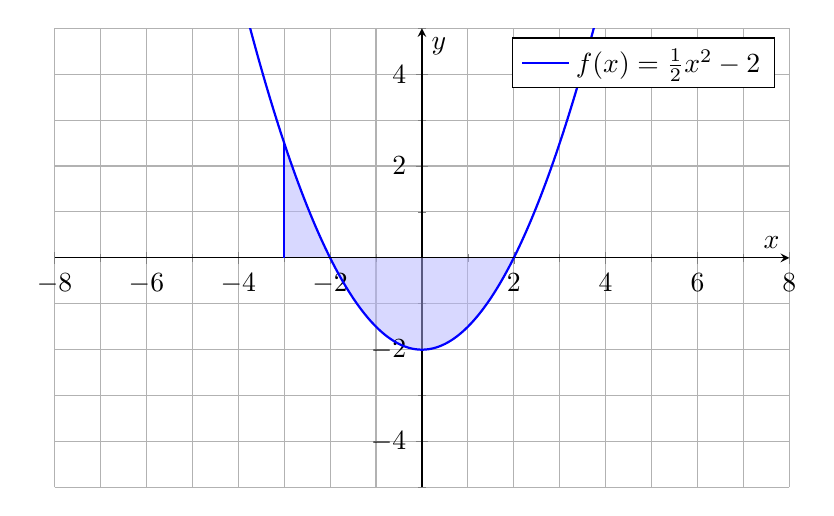
\begin{tikzpicture}
\begin{axis}[
    axis lines = middle,
    xlabel = $x$,
    ylabel = $y$,
    xmin=-8, xmax=8,
    ymin=-5, ymax=5,
    axis equal image,
    width=0.9\textwidth,
    grid=both,
    minor tick num=1,
    major grid style={gray!60},
    minor grid style={gray!60}
]

% Funktion
\addplot[name path=f, blue, thick, domain=-6:6, samples=200] {(1/2)*x^2-2};
\addlegendentry{$f(x)=\frac{1}{2}x^2-2$}

% x-Achse als zweite Kurve
\addplot[name path=xaxis, domain=-3:2] {0};

% Fläche zwischen Funktion und x-Achse
\addplot[
    blue!30,
    opacity=0.5
] fill between[
    of=f and xaxis,
    soft clip={domain=-3:2},
];
\addplot[blue, thick] coordinates {(-3,2.5) (-3,0)};
\end{axis}
\end{tikzpicture}
\end{center}
Offenbar müssen wir zuerst die Nullstellen bestimmen: Hier erhalten wir $x_{1/2}=\pm 2$. Wir teilen den Intervall $I$ auf in $I_1=[-3,-2]$ und $I_2=[-2,2]$. Daraus folgt für den Flächeninhalt:
\[ A = \mleft| [F(x)]_{-3}^{-2}  \mright| + \mleft| [F(x)]_{-2}^2  \mright| = \mleft| \dfrac{8}{3}- \dfrac{3}{2} \mright| + \mleft| - \dfrac{16}{3} \mright| = \num{6,5}\]
mit der Stammfunktion $F(x)=\dfrac{1}{6}x^3-2x$. Schritte 2.\ und 3.\ kann man, wie oben gesehen, auch in Einem machen. Sicherer ist aber das Abarbeiten der Teilschritte, um Flüchtigkeitsfehler zu vermeiden, und die Übersicht zu behalten.
\end{example}

Einen Schritt weiter gedacht ist kann man auch den Flächeninhalt zweier Funktionsgraphen mit diesem Verfahren ermitteln. Es gilt:

\begin{theorem} \textbf{(Berchnung des Flächeninhalts zweier Funktionsgraphen)}
\begin{enumerate}
\item Der Inhalt $A$ einer Fläche, die im Intervall $I=[a,b]$ von den Graphen zweier Funktionsgraphen $f$ und $g$ begrenzt wird, wobei stets $f(x)\geq g(x)$ bzw.\ $g(x)\geq f(x)$ gilt, berechnet man mit
\[ A= \mleft| \int_a^b (f(x)-g(x))\diff x   \mright|. \]
\item Zur Berechnung bestimmt man zuerst alle Schnittstellen $x_k$ der Graphen im Intervall $I$. Anschließend werden die Teilabschnitte wie in Satz \ref{Satz:Int_FlächeX} addiert.
\end{enumerate}
\index{Flächeninhalt!Berechnung zwischen zwei Graphen}
\end{theorem}


\begin{example}
Betrachten wir die Funktionsgraphen $f(x)=\dfrac{1}{2}x+1$, $g(x)=-\dfrac{1}{4}x^2+4$ und den Intervall $I=[-4,4]$.


\begin{center}
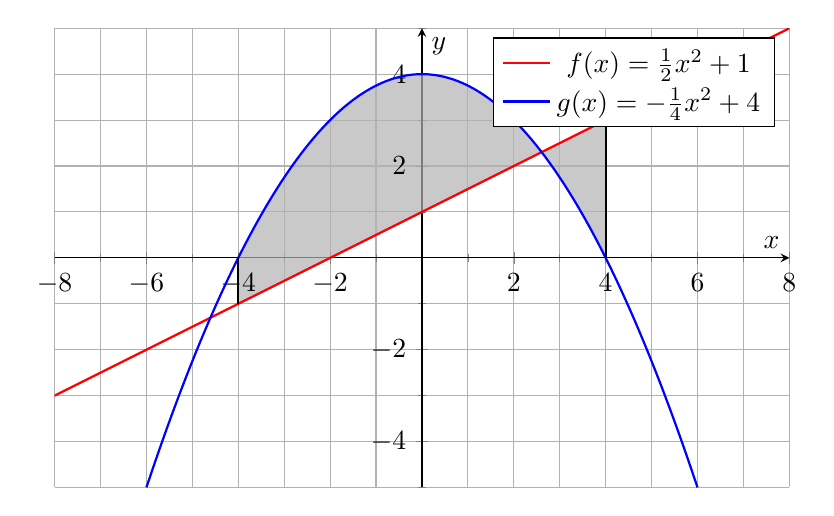
\begin{tikzpicture}
\begin{axis}[
    axis lines = middle,
    xlabel = $x$,
    ylabel = $y$,
    xmin=-8, xmax=8,
    ymin=-5, ymax=5,
    axis equal image,
    width=0.9\textwidth,
    grid=both,
    minor tick num=1,
    major grid style={gray!60},
    minor grid style={gray!60}
]

% Funktion
\addplot[name path=f, red, thick, domain=-9:9, samples=200] {(1/2)*x+1};
\addlegendentry{$f(x)=\frac{1}{2}x^2+1$}

\addplot[name path=g, blue, thick, domain=-6:6, samples=200] {(-1/4)*x^2+4};
\addlegendentry{$g(x)=-\frac{1}{4}x^2+4$}

% Fläche zwischen Funktion und x-Achse
\addplot[
    black!30,
    opacity=0.7
] fill between[
    of=f and g,
    soft clip={domain=-4:4},
];
\addplot[black, thick] coordinates {(-4, 0) (-4,-1)};
\addplot[black, thick] coordinates {(4,0) (4,3)};
\end{axis}
\end{tikzpicture}
\end{center}
Nun bestimmen wir den Flächeninhalt, den die Funktionen einschließen. Dazu bestimmen wir den Schnittpunkt:
\[ \frac{1}{2}x+1 = -\frac{1}{4}x^2+4 \Leftrightarrow x_{1/2} = -1 \pm \sqrt{13},  \]
indem wir beispielsweise die Mitternachtsformel verwenden. Dabei fällt eine Lösung weg, da $-1-\sqrt{13} \approx -\num{4,6} < -4$ außerhalb des Intervalls liegt. Nun berechnen wir den Flächeninhalt in Teilabschnitten:
\[ A = A_1+A_2 = \mleft| \int_{-4}^{-1+\sqrt{13}} \mleft(-\dfrac{1}{4}x^2-\dfrac{1}{2}x+3 \mright) \diff x \mright| + \mleft| \int_{-1+\sqrt{13}}^{4} \mleft(-\dfrac{1}{4}x^2-\dfrac{1}{2}x+3 \mright) \diff x \mright| \]
\[ = \mleft| \dfrac{13\sqrt{13}-19}{6} - \mleft( - \dfrac{32}{3} \mright)   \mright| + \mleft| \dfrac{8}{3} - \dfrac{13\sqrt{13}-19}{6}  \mright| = \dfrac{5+13\sqrt{13}}{3} \approx \num{17,29}  \]
\end{example}

%\subsubsection{Uneigentliche Inegrale}
\begin{definition}
Existiert für eine im Intervall $[a,\infty[$ bzw. $]a,b]$ definierte Funktion $f$
\[ \lim_{z\to \infty} \int_a^zf(x)\diff x = \int_a^\infty f(x)\diff x \hspace{1cm} \text{bzw.} \hspace{1cm} \lim_{z\to a} \int_z^bf(x)\diff x = \int_a^bf(x)\diff x,\]
so nennt man diesen Grenzwert \textbf{uneigentliches Integral} über dem Intervall. Die Schreibweisen auf der rechten Seite des Gleichheitszeichens sind dabei Kurzschreibweisen, die aber das gleiche meinen.
\index{Integral!Uneigentliches} \index{Uneigentliches Integral}
\end{definition}

\begin{example} \
\begin{enumerate}
\item Betrachten wir das uneigentliche Integral $\displaystyle \int_{-\infty}^0 e^x \diff x$, so gilt zu überprüfen, ob der Grenzwert $\lim\limits_{x\to - \infty} e^x$ für $e^x$ als Stammfunktion existiert, also endlich ist. Durch Nachrechnen kann gezeigt werden, dass $\lim\limits_{x\to - \infty} e^x = 0$ ist. Wir setzen ein:
\[ \lim_{z\to -\infty} \int_z^0 e^x \diff x = \lim_{z\to -\infty} [e^x]_z^0 = e^0 - 0 = 1\]
\item Nicht definiert ist hingegen das Integral $\displaystyle \int_0^\infty e^x \diff x$, denn die Stammfunktion $e^x$ geht für $x\to \infty$ gegen unendlich. Der Grenzwert ist nicht definiert, und dadurch existiert das uneigentliche Integral nicht.
\item Spannend ist der Fall $f(x)=\dfrac{1}{\sqrt{x}}$ mit $\displaystyle \int_1^\infty f(x) \diff x$. Eine Stammfunktion hierbei ist $F(x)=\sqrt{x}$, was bedeutet, dass die Fläche für große x-Werte unendlich groß wird. Auch hier ist das uneigentliche Integral nicht definiert.
\item Obwohl die Funktion $g(x)=\dfrac{1}{x^2}$ sehr ähnlich zu $f(x)$ verläuft, ist hier das uneigentliche Integral $\displaystyle \int_{1}^\infty g(x) \diff x$ definiert. Denn eine Stammfunktion ist $G(x)=-\dfrac{1}{x}$, und der Grenzwert $\lim\limits_{x\to \infty}G(x)=0$ existiert. Wir berechnen also das uneigentliche Integral:
\[ \int_1^\infty g(x) \diff x = \lim_{a\to\infty} G(a)-G(1)=0- (-1)=1\]
\begin{center}
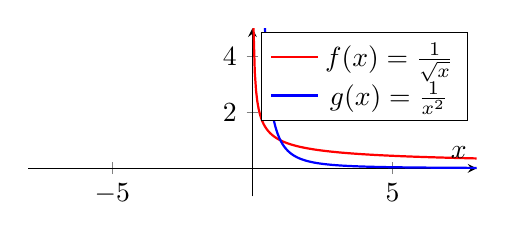
\begin{tikzpicture}
\begin{axis}[
    axis lines = middle,
    xlabel = $x$,
    ylabel = $y$,
    xmin=-8, xmax=8,
    ymin=-1, ymax=5,
    axis equal image,
    width=0.6\textwidth,
]

% Funktion
\addplot[name path=f, red, thick, domain=0.04:9, samples=200] {x^(-1/2)};
\addlegendentry{$f(x)=\frac{1}{\sqrt{x}}$}
\addplot[name path=f, blue, thick, domain=0.2:9, samples=200] {1/x^2};
\addlegendentry{$g(x)=\frac{1}{x^2}$}

\end{axis}
\end{tikzpicture}
\end{center}

\end{enumerate}
\end{example}

%\subsubsection{Das Integral als Gesamtänderung einer Größe}
Im Lehrplan ders Gymnasiums wird noch ein bisschen Anwedungspraxis gefordert, denn die aktuelle Behandlung mit Integralen war sehr mathematisch. Als ersten der zwei Anwendungsfälle ist die Betrachtung als Gesamtänderung einer Zustandsgröße zu nennen. Hierbei betrachtet man eine Funktion, die die momentane Änderungsrate einer Zustandgröße angibt, und fragt sich nun nach der Gesamtänderung der Größe in Abhängigkeit der Zeit. Dabei gilt folgender Zusammenhang:

\begin{theorem} \textbf{(Über Zustandsgrößen und deren Gesamtänderung)}
\begin{enumerate}
\item Beschreibt die Funktion $f(t)$ eine Zustandsgröße in Abhängigkeit der Zeit (oder einer anderen Größe), so gilt für die \textit{momentante Änderungsrate} der Zustandsgröße $y=f'(t)$.
\item Beschreibt $f(t)$ bereits die momentante Änderung der Zustandsgröße, so entspricht der Gesamtänderung der Zustandsgröße im Intervall $[a,b]$ das Integral
\[ \int_a^bf(t)\diff t.\]
\item Die Integralfunktion $\displaystyle I_a(x)=\int_a^xf(t)\diff t$ beschreibt die absolute Zustandsänderung ab dem Zeitpunkt $x=a$.
\end{enumerate}
\index{Zustandsgröße} \index{Änderungsrate}
\end{theorem}

Ein Anwendungsbeispiel aus der Physik, das der Lehrplan aber für die Mathematik vorsieht, ist der Zusammenhang zwischen Strecke und Geschwindigkeit.

\begin{example}
Wir betrachten die Strecke von A-Dort nach B-Stadt, die ein Güterzug zurücklegt. Diese wird durch die Funktion $s(t)=\dfrac{1}{5}t^5-1.5t^4+3t^3$ beschrieben, wobei $t\in [0,3]$, $t$ in Stunden, ist. Für $t=0$ ist der Zug in A-Dorf, und zu $t=3$ kommt der Zug in B-Stadt an. Ein Funktionswert von $1$ entspricht dabei $\SI{10}{\kilo\meter}$. Nun wollen wir wissen, wie schnell der Güterzug zu einem gegebenen Zeitpunkt gefahren ist. Dafür nutzen wir die Ableitung, denn diese gibt an, wie viel sich die Strecke pro Zeit geändert hat. Wir ermitteln: 
\[ s'(t) = v(t)=t^4-6t^3+9t^2\]
Eine Stunde nach Abfahrt ist der Zug beispielsweise $v(1)=3$ schnell. Da der Funktionswert von $y=3$ für die Strecke eine Länge von $\SI{10}{\kilo\meter}$ bedeutet hat und wir nach der Zeit abgeleitet haben, also die Änderung der Strecke \textit{pro Stunde} betrachten, dividieren wir den Maßstaab durch $\SI{1}{\hour}$ und erhalten so mit Einheiten:
\[ v(1) = 3 \cdot \dfrac{\SI{10}{\kilo\meter}}{\SI{1}{\hour}} = \SI{30}{\kilo\meter\per\hour}\]
Der Zug fährt also eine Stunde nach Abfahrt in A-Dort mit einer Geschwindigkeit von $\SI{30}{\kilo\meter\per\hour}$. \par
Die Rückrichtung von Geschwindigkeit zu Weg erhalten wir durch die Integralfunktion. Wir integrieren die Geschwindigkeitsfunktion, und für die Integralfunktion $I_1$, die die Änderung des Weges zum Zeitpunkt $t=1$ beschreibt, ermitteln wir beispielsweise:
\[ \int v(t) \diff t = \dfrac{1}{5}t^5 - \dfrac{3}{2}t^4+3t^2 + c\]
Nullstelle für $x=1$, damit wir eine Integralfunktion haben:
\[ 0 = \dfrac{1}{5}-\dfrac{3}{2}+3+c \Leftrightarrow c = -\num{1,7}\]
\[ \Rightarrow I_1(t) = \dfrac{1}{5}t^5 - \dfrac{3}{2}t^4+3t^2 -\num{1,7}\]
\begin{center}
\begin{tikzpicture}
\begin{axis}[
    axis lines = middle,
    xlabel = $t$ in $\unit{\hour}$,
    ylabel = $y$,
    xmin=-1, xmax=12,
    ymin=-2, ymax=9,
    axis equal image,
    width=0.7\textwidth,
]

% Funktion
\addplot[name path=v, red, thick, domain=0:3, samples=200] {x^4-6*x^3+9*x^2};
\addlegendentry{$v(t)$ in $\SI{10}{\kilo\meter\per\hour}$}
\addplot[name path=s, black, thick, domain=0:3, samples=200] {(1/5)*x^5-(3/2)*x^4+3*x^3};
\addlegendentry{$s(t)$ in $\SI{10}{\kilo\meter}$}
\addplot[name path=I, blue, thick, domain=0:3, samples=200] {(1/5)*x^5-(3/2)*x^4+3*x^3-1.7};
\addlegendentry{$I_1(t)$ in $\SI{10}{\kilo\meter}$}

\end{axis}
\end{tikzpicture}
\end{center}
Zusammengefasst also: Wenn wir die Geschwindigkeit integrieren, erhalten wir die Strecke. Andersherum ist die Geschwindigkeit die Ableitung der Strecke.
\end{example}

%\subsubsection{Volumen von Rotationskörpern}

\begin{theorem} \textbf{(Volumen eines Rotationskörpers)} \par
Sei die Funktion $f$ im Intervall $[a,b]$ stetig. Rotiert ein Körper, der durch die Funktion $f$ nach außen hin begrenzt wird, um die x-Achse, so entsteht ein Rotationskörper mit Volumen
\[ V=\pi \cdot \int_a^b(f(x))^2 \diff x\]
\label{Satz:Vol_RotK}
\index{Volumen!eines Rotationskörpers}
\index{Rotationskörper}
\end{theorem}

\begin{example}
Gegeben ist die Funktion
$f(x)=x \quad \text{für } 0 \le x \le 2.$
Der Graph wird nun um die x-Achse rotiert, wobei wir das Volumen des dabei entstandenen Rotationskörpers ermitteln wollen. Zuerst quadrieren wir $f(x)^2=x^2$. Nun setzen wir in die Formel zur Berechnung ein:
\[
V=\pi \int_0^2 x^2\,dx
=\pi\left[\frac{x^3}{3}\right]_0^2
=\frac{8\pi}{3}.
\]

\[
\Rightarrow V=\frac{8\pi}{3}
\]

\begin{center}
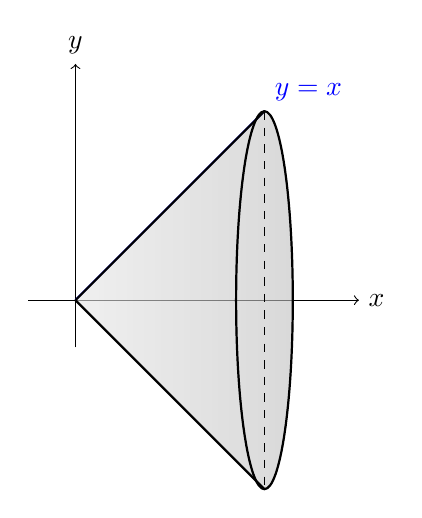
\begin{tikzpicture}[scale=1.2]

  % Achsen
  \draw[->] (-0.5,0,0) -- (3,0,0) node[right] {$x$};
  \draw[->] (0,-0.5,0) -- (0,2.5,0) node[above] {$y$};

  % Funktion y = x
  \draw[thick, blue] (0,0) -- (2,2) node[above right] {$y=x$};

  % Parameter
  \def\R{2}   % Radius bei x=2
  \def\L{2}   % Länge

  % Mantelfläche (Schattierung)
  \shade[left color=gray!20, right color=gray!50, opacity=0.6]
    (0,0) -- (2,2)
    arc[start angle=90,end angle=-90,x radius=0.3,y radius=2]
    -- cycle;

  % Vordere Mantellinie
  \draw[thick] (0,0) -- (2,2);
  \draw[thick] (0,0) -- (2,-2);

  % Hintere Mantellinie gestrichelt
  \draw[dashed] (2,2) -- (2,-2);

  % Grundellipse bei x=2
  \draw[thick] (2,0) ellipse [x radius=0.3, y radius=2];
  \draw[dashed] (2,0) ellipse [x radius=0.3, y radius=2];


\end{tikzpicture}
\end{center}
\end{example}

\newpage

\section{Algebraische Grundlagen}
In diesem kleinen Kapitel soll es um Elemente der Algebra gehen. Die Algebra ist im Kern die Teildisziplin der Mathematik, in der Gleichungen und Variablen behandelt werden. Wir betrachten hier also Lösungswege für (Un-)Gleichungen und wiederholen dabei ein paar Elemente der Mittelstufe.
\subsection{Binomische Formeln}
Ein wohl wichtiges Element der Mittelstufe sind die binomischen Formeln. Sie sind zwar in der Merkhilfe angegeben, doch auch im Prüfungsteil A des Abiturs können sie Verwendung finden.
\begin{theorem} \textbf{(Binomische Formeln)} \par
Sind $a,b\in \R$ beliebig. Dann gilt:
\begin{enumerate}
\item $(a+b)^2=a^2+2ab+b^2$
\item $(a-b)^2=a^2-2ab+b^2$
\item $(a+b)\cdot (a-b)=a^2-b^2$
\end{enumerate}
\index{Formel!Binomische} \index{Binomische Formeln}
\end{theorem}
Es empfiehlt sich dringlichst, sich die Formeln gut einzuprägen!

\begin{example}
Ein Anwendungsfall ist das Quadrieren im Kopf. Solle man $52^2$ berechnen, so ist das eine mühselige Aufgabe, doch mit der 1. binomischen Formel geht das recht elegant: 
\[ 52^2 = (50+2)^2 = 50^2+2\cdot 50 \cdot 2 + 2^2 = 2500 + 200 + 4 = 2704\]
Nun könnten wir analog dazu $49^2$ wiefolgt berechnen:
\[ 49^2 = (50-1)^2 = 2500 - 100 +1 = 2401\]
Die dritte binomische Formel ist meist in Anwendung, wenn man von einerm Term wie $25-16$ in einzelne Faktoren zerlegen will. Hier sieht man schnell: 
\[ 25-16 = 5^2-4^2 = (5-4)\cdot (5+4) = 1 \cdot 9 = 9\]
\end{example}

\newpage

\subsection{Gleichungssysteme}
Gleichungssysteme sind normalerweise mehrere Gleichungen, wobei es dort immer Variablen zu bestimmen gilt. Im Normalfall ist vieles von dem, was wir in der Analysis tun, auf Gleichungen zurückzuführen. So bestimmen wir Nullstellen, Extrema etc.\ mit Gleichungen, da wir einen gegeben Term gleich Null setzen. Mehrere Gleichungen als ein Gleichungssystem kennen wir nur mit linearen Gleichungen, beispielsweise in der Vektorgeometrie. 

%\subsubsection{Äquivalenzumformungen für (Un-)Gleichungen}

\begin{theorem}\textbf{(Äquivalenzumformungen für Gleichungen)} \par
Für jede Gleichung gelten die folgenden Äquivalenzumformungen:
\begin{enumerate}
\item Auf beiden Seiten darf ein beliebiger Term $T(x)$ addiert oder subtrahiert werden.
\item Auf beiden Seiten darf mit einer beliebigen reellen Zahl $\lambda \in \R \setminus \{ 0 \}$ multipliziert werden.
\end{enumerate}
\index{Äquivalenzumformungen!für Gleichungen}
\end{theorem}

\begin{theorem}\textbf{(Äquivalenzumformungen für Ungleichungen)} \par
Für jede Ungleichung gibt es die folgenden Äquivalenzumformungen:
\begin{enumerate}
\item Auf beiden Seiten darf ein beliebiger Term $T(x)$ addiert oder subtrahiert werden.
\item Eine Ungleichung darf mit einer beliebigen positiven Zahl multipliziert oder dividiert werden.
\item Eine Ungleichung darf auch mit einer negativen Zahl multipliziert und dividiert werden. Dabei ändern sich aber die \textit{Relationszeichen} der Ungleichung:
\begin{center}
Aus $<$ wird $>$, \hspace{3cm}
aus $>$ wird $<$, \par
aus $\leq$ wird $\geq$, \hspace{3cm}
aus $\geq$ wird $\leq$.
\end{center}
\end{enumerate}
\index{Äquivalenzumformungen!für Ungleichungen}
\end{theorem}

Die hier genannten Regeln werden implizit in den Beispielen weiter unten verwendet. Explizit wird hier also kein Beispiel genannt.

%\subsubsection{Lineare Gleichungen}
\begin{theorem}
Eine lineare Gleichung vom allgemeinen Typ
\[ a\cdot x + b = 0\]
mit gesuchter Variable $x$ besitzt \emph{genau eine} Lösung bei $x=-\dfrac{b}{a}$.
\index{Lineare Gleichung}
\end{theorem}

\begin{example}
Betrachten wir die lineare Gleichung vom Typ $4x +2 = -2$, so bestimmen wir die Lösung, indem wir nach x auflösen. Zum Beispiel durch
\[ 4x+2=-2 \Leftrightarrow 4x = -4 \Leftrightarrow x = -1\]
Also ist $x=-1$ unsere Lösung. Die Lösungsmenge, falls gefragt, geben wir an durch:
\[ \Lsg = \{ 1 \}  \]
\end{example}

%\subsubsection{Quadratische Gleichungen}

\begin{theorem} \textbf{(Lösungsformeln für quadratische Gleichungen)}
\begin{enumerate}
\item \textbf{Mitternachtsformel:}\index{Mitternachtsformel} Sei eine quadratische Form der Art $ax^2+bx+c=0$ mit reellen Koeffizienten $a,b,c\in \R, a\neq 0$ gegeben. Dann heißt $D=b^2-4ac$ die \textbf{Diskriminante}\index{Diskriminante}. Für $D<0$ ist die Gleichung auf den reellen Zahlen nicht lösbar. Für $D\geq 0$ erhalten wir die Lösungen
\[ x_{1/2}=\dfrac{-b\pm \sqrt{D}}{2a} = \dfrac{-b \pm \sqrt{b^2-4ac}}{2a}  \]
Ist $D=0$, so erhalten wir exakt eine Lösung. Für $D>0$ gibt es genau zwei.
\item \textbf{p-q-Formel:}\index{p-q-Formel} Sei eine quadratische Form der Art $x^2+px+q=0$ mit reellen Koeffizienten $p,q \in \R$ gegeben. Dann lauten die Lösungen der quadratischen Gleichung
\[ x_{1/2} = -\dfrac{p}{2}\pm \sqrt{\mleft(\dfrac{p}{2}\mright)^2-q}  \]
Auch hier gilt, ist der Radikant kleiner als null, so existieren keine Lösungen. 
\end{enumerate}
\label{Satz:MNF_PQ}
\end{theorem}

Man kann die Mitternachtsformel durch Division mit $a$ in die Form für die p-q-Formel bringen. Die Lösung ändert sich dabei nicht. Die p-q-Formel steht in der Formelsammlung, die Mitternachtsformel nicht. Es empfiehlt sich aber, letztere zu lernen, da sie universeller einsetzbar ist, und man sich einen Rechenschritt spart. 

\begin{example}

Betrachten wir die quadratische Gleichung $2x^2+4x=6$, dann lösen wir die Gleichung auf zwei Wege.
\begin{enumerate}
\item $2x^2+4x=6 \Leftrightarrow 2x^2+4x-6=0$. Einsetzen in die Mitternachtsformel liefert uns:
\[ x_{1/2} = \dfrac{-4\pm \sqrt{4^2-4 \cdot 2 \cdot (-6)}}{2\cdot 2} = \dfrac{-4 \pm 8}{4} = -1 \pm 2\]
Also insbesondere $\Lsg = \{ -3, 1\}$.
\item $2x^2+4x=6$ formen wir in die Form für die p-q-Formel um: $2x^2+4x=6 \Leftrightarrow x^2+2x-3=0$. Einsetzen ergibt
\[ x_{1/2} = -\dfrac{2}{2} \pm \sqrt{\mleft( \dfrac{2}{2}\mright)^2 - (-3)} = -1 \pm \sqrt{1^2+3} = -1 \pm 2  \]
Auch hier erhalten wir also die Lösungsmenge $\Lsg = \{ -3, 1\}$.
\end{enumerate}
\label{Bsp:Quadrat_Gl}
\end{example}

%\subsubsection{Kubische und Biquadratische Gleichungen}
Für höhere Potenzen werden Lösungen immer schwerer zu finden. Für die folgenden zwei Sonderfälle gibt es aber Lösungen. 
\begin{theorem}
\begin{enumerate}
\item Sei $ax^3+bx^2+cx=0$ eine kubische Gleichung mit $a,b,c \in \R, a\neq 0$. Dann gilt:
\[ ax^3+bx^2+cx = x \cdot (ax^2+bx+c) = 0  \]
Die \emph{triviale} Lösung $x=0$ ist also immer möglich. Weitere Lösungen können durch die Lösung einer quadratischen Gleichung nach Satz \ref{Satz:MNF_PQ} bestimmt werden. 
\item Die Gleichung $ax^4+bx^2+c=0$ mit $a,b,c\in \R, a\neq 0$ heißt \textbf{biquadratische Gleichung}. Lösungen erhält man durch Substitution $x^2=u$, sodass 
\[ ax^4+bx^2+c= 0 \Leftrightarrow au^2+bu+c = 0\]
gilt und man nun die Lösungen in Abhängigkeit von $u$ bestimmt. Durch Rücksubstitution $x_{1/2}=\pm\sqrt{u_1}, x_{3/4}=\pm \sqrt{u_2}$ erhält man bis zu vier Lösungen.
\end{enumerate}
\index{Biquadratische Gleichungen} \index{Kubische Gleichungen}
\end{theorem}

\begin{example} \
\begin{enumerate}
\item Sei $2x^3+4x2-6x=0$ die betrachtete kubische Gleichung. Dann ist $x=0$ die \emph{triviale} Lösung. Die anderen Beiden Lösungen folgen analog zu Beispiel \ref{Bsp:Quadrat_Gl}. Also $\Lsg = \{ -3, 0, 1\}$.
\item Für $x^4+2x^2-3=0$ Substituieren wir mit $u=x^2$ zu $0=u^2+2u-3$. Die Lösungen folgen nach \ref{Bsp:Quadrat_Gl}: $u_1=-3, u_2 = 1$. Durch Rücksubstitution müssten wir die Wurzel aus $u_1$ ziehen, doch das ist nicht möglich. Deshalb bleiben nur $x_{3/4}=\pm \sqrt{1} = \pm 1$. Also ist hier die Lösungsmenge bestehend aus $\Lsg = \{ -1, 1\}$. 
\end{enumerate}
\end{example}

%\subsubsection{Bruchgleichungen}
\begin{theorem} \textbf{(Lösen von Bruchgleichungen)} \par
Zum Lösen einer Bruchgleichung multipliziert man mit den Nennern. Anschließend formt man die Gleichung strategisch um und nutzt bekannte Lösungsschemata.
\index{Bruchgleichung}
\end{theorem}
Dieser Satz ist bewusst sehr allgemein gehalten, denn wie genau man das im Beispiel umsetzt, kann man schwer sagen. Wir wollen uns deshalb ein paar konkrete Anwendungsfälle ansehen.

\begin{example} \
\begin{enumerate}[1.]

\item Sei eine Bruchgleichung der Form $\dfrac{x}{x+1} = \dfrac{2x}{x-5}$ gegeben. Umformen liefert uns:
\[ \dfrac{x}{x+1} = \dfrac{2x}{x-5} \Leftrightarrow x(x-5) = 2x(x+1) \Leftrightarrow x^2-5x = 2x^2+2x \Leftrightarrow -x^2 -7 = 0  \]
Das Nutzen der Mitternachtsformel wäre hier möglich, doch durch geschicktes hinsehen kommt man viel einfacher auf die Lösung:
\[ -x^2-7=0 \Leftrightarrow x^2 = 7 \Rightarrow x=\pm \sqrt{7} \]
Dabei gilt es stets, das Plus-Minus vor der Wurzel zu beachten!

\item Gegeben sei die Bruchgleichung $\dfrac{-4x^2+2}{x}=\num{0,5}$. Auch hier formen wir um zu
\[ \dfrac{-4x^2+2}{x} = \dfrac{1}{2} \Leftrightarrow -4x^2+2 = \dfrac{1}{2} x \Leftrightarrow -4x^2-\dfrac{1}{2} x + 2 = 0 \Rightarrow x_{1/2}=\dfrac{-1\pm \sqrt{129}}{16} \]

\end{enumerate}

\end{example}

%\subsubsection{Wurzelgleichungen}
\begin{definition}
Sei $n\geq 1$ eine natürliche Zahl und $a\geq 0$, so besitzt die Gleichung
\[ x^n=a\]
genau eine nichtnegative reelle Lösung. Diese wird als $n$-te Wurzel aus $a$ bezeichnet. Man schreibt dafür:
\[ x = \sqrt[n]{a}\]
Hierbei bezeichnet man
\begin{itemize}
\item $\sqrt[n]{a}$ als Wurzel,
\item $\sqrt{}$ als Wurzelzeichen,
\item $n$ als Wurzelexponent,
\item $a$ als Radikand. 
\end{itemize}
\index{Wurzel!Definition}
\end{definition}
Eine wichtige Bemerkung, die deshalb hier betont werden soll (!), ist der Unterschied einer Wurzel und der Lösung einer quadratischen Gleichung. Während man die Wurzel einer konkrete Zahl $a$ stets positiv und eindeutig angibt, so existieren bei quadratischen Funktion/Gleichung auch oft zwei verschiedene Lösungen (deshalb das Plus-Minus-Zeichen). Anhand eines Beispiels wird der Sachverhalt deutlich:

\begin{example} \ 
\begin{enumerate}
\item Die (Quadrat-)Wurzel aus $4$ ist die nichtnegative Zahl $\sqrt{4}=2$. 
\item Die Lösung der quadratischen Gleichung $x^2=4$ ist $x=\pm \sqrt{4}=\pm 2$, denn beide Lösungen führen zum Ergebnis von $4$. 
\item Auch die Zahl $\sqrt{0}$ ist definiert. Für sie gilt: $\sqrt{0}=0$.
\item $\sqrt{-3}$ ist nicht definiert, der Ausdruck ergibt keinen Sinn. Denn keine reelle Zahl quadriert ergibt $-3$. 
\item Zwar würde der Ausdruck $\sqrt[3]{-8}$ Sinn ergeben, denn $(-2)^3=-8$. Nach unserer Definition fordern wir allerdings Radikanten, die nicht negativ sein dürfen, und offensichtlich ist $-8<0$. Da diese Erweiterung allerdings kein Problem darstellt, kann man diesen Ausdruck mathematisch korrekt angeben. Selbst Mathematiker sind sich nicht einig, aber beide Positionen, definiert oder nicht, sind vertreten. Für gerade Wurzelexponenten $n$ muss der Radikant zwingend größer oder gleich mit $0$ sein.
\end{enumerate}
\index{Wurzelgleichung}
\end{example}

%\subsubsection{Logarithmusgleichungen}

\begin{theorem} \textbf{(Lösungsstrategie für Logarithmusgleichungen)} \par
Betrachtet man eine Logarithmusgleichung 
\[ a^x = b\]
mit $a,b>0$, so erhält man die Lösung durch die Anwendung des natürlichen Logarithmus wiefolgt:
\begin{enumerate}
\item $a^x = b \Rightarrow \ln (a^x) = \ln (b)$. Mit Potenzgesetzen ziehen wir das $x$ vor den Logarithmus und Schritt zwei in Schritt zwei formt man weiter um zu
\item $\ln (a^x) = \ln (b) \Rightarrow x \ln(a) = \ln (b) \Rightarrow x = \dfrac{\ln(b)}{\ln(a)}$.
\end{enumerate}
Die Lösung zur o.g. Gleichung lautet also
\[ x=\dfrac{\ln b}{\ln a}\]
\index{Logarithmusgleichung}
\label{Satz:LogGleichung}
\end{theorem}
Wir forderten zwar die Verwendung des natürlichen Logarithmus. Tatsächlich darf man jeden beliebigen Logarithmus nutzen - Der $\ln$ bietet sich an, weil er im Zusammenhang mit der $e$-Funktion sowieso oft in Verwendung ist.

\begin{example}
Sei die Lösung der Gleichung $\mleft(\dfrac{1}{2}\mright)^x = \num{0,1}$ gesucht, so erhalten wir diese Lösung mittels der Strategie aus Satz \ref{Satz:LogGleichung}. Dazu gehen wir wiefolgt vor:
\[ \mleft(\dfrac{1}{2}\mright)^x = \num{0,1} \Leftrightarrow x \cdot \ln (\num{0,5}) = \ln(\num{0,1}) \Leftrightarrow x = \dfrac{\ln(\num{0,1})}{\ln (\num{0,5})} \approx \num{3,3219281} \]
\end{example}

\newpage
\section{Elementargeometrie}
In diesem kleinen Kapitel sollen alle geometrischen Erkenntnisse bis zum Ende der Mittelstufe wiederholt werden, die man im Abitur gebrauchen könnte. Für das Abitur sind diese Inhalte relativ unbedeutend, sind aber vereinzelt in Aufgben abverlangt. Der Fokus sollte in jedem Fall im Folgekapitel zur analytischen Geometrie / Linearen Algebra liegen, da dort der Großteil der Geometrie behandelt wird, der für das Abitur einen direkten Einfluss hat. Ein kurzes Überfliegen dieses aktuellen Kapitels schadet allerdings nicht, und kann nochmals einige Inhalte in den Kopf rufen.

\subsection{Geometrie der Figuren und Körper}

Zuerst wollen wir Grundbegriffe aus der Unterstufe wiederholen, die du fürs Abitur beherrschen solltest.

\begin{definition} \textbf{(Grundbegriffe der Geometrie)}
\begin{enumerate}
\item Ein Punkt\index{Punkt} ist ein geometrisches Objekt, dass eine Position hat. Ein Punkt hat Koordinaten und wird mit $A(x|y)$ bzw. $A(x_1|x_2|x_3)$ angegeben.
\item Eine Strecke\index{Strecke} ist die kürzeste Verbindung von zwei Punkten. Die Strecke zwischen $A$ und $B$ wird mit $|\overline{AB}|$ bezeichnet.
\item Eine Gerade\index{Gerade!in der Elementargeometrie} ist eine unendlich lange Linie. Die Gerade durch die Punkte $A$ und $B$ schreibt man auch als $\overline{AB}$.
\item Als Halbgerade\index{Halbgerade} wird eine Strecke bezeichnet, die sich zu einer Seite unendlich ausbreitet, zur anderen Seite aber durch einen Punkt begrenzt ist. Ist $A$ dieser Punkt und verläuft die Halbgerade durch den Punkt $B$, so schreibt man für die Halbgerade auch $[AB$.
\item Sei $M$ ein Punkt. Dann heißt die Menge aller Punkte, die den gleichen Abstand zu $M$ haben, Kreis\index{Kreis} um den Mittelpunkt $M$.
\end{enumerate}
\label{Def:Euklid_Objekte}
\end{definition}

\begin{example} In der untenstehenden Abbildung ist die Strecke $|\overline{AB}|$ abgebildet. Durch den Mittelpunkt $B$ wird ein Kreis erzeugt. Eine Halbgerade erstreckt sich gestrichelt von $A$ in Richtung $C$. Eine Gerade ist durch $\overline{CB}$ abgebildet:
\begin{center}
\begin{tikzpicture}[scale=1]

% Punkte
\coordinate (A) at (1,1);
\coordinate (B) at (5,1);
\coordinate (C) at (2,4);

% Strecke AB
\draw[thick] (A) -- (B);

% Gerade AC (verlängert)
\draw[thick, dashed] (A) -- ($(A)!1.5!(C)$);

% Gerade BC (unendlich verlängert in beide Richtungen)
\draw[thin] ($(B)!-1!(C)$) -- ($(B)!1.5!(C)$);

% Kreis um B mit Radius 2
\draw (B) circle (2);

% Punkte markieren
\fill (A) circle (2pt) node[below left] {$A$};
\fill (B) circle (2pt) node[above right] {$B$};
\fill (C) circle (2pt) node[above] {$C$};

\end{tikzpicture}
\end{center}
\end{example}

Als nächstes beschäftigen wir uns intensiver mit Dreiecken. Die Definition eines Dreiecks ist vermutlich relativ offensichtlich, dennoch sei sie hier kurz ausgeführt:

\begin{definition}
Ein Dreieck besteht aus drei Punkten, die nicht auf einer Geraden liegen. Die Punkte des Dreiecks heißen Ecken. Die Verbindungslinien, also die Strecken zwischen den Punkten, heißen Seiten. Man verwendet folgende Notation:
\begin{center}
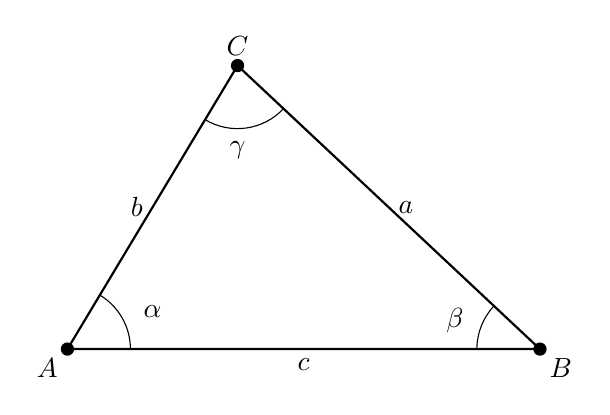
\begin{tikzpicture}[scale=1.2]

% Punkte
\coordinate (A) at (0,0);
\coordinate (B) at (5,0);
\coordinate (C) at (1.8,3);

% Dreieck
\draw[thick] (A) -- (B) -- (C) -- cycle;

% Seitenbezeichnungen
\node[below] at ($(A)!0.5!(B)$) {$c$};
\node[left]  at ($(A)!0.5!(C)$) {$b$};
\node[right] at ($(B)!0.5!(C)$) {$a$};

% Eckpunkte
\fill (A) circle (2pt) node[below left] {$A$};
\fill (B) circle (2pt) node[below right] {$B$};
\fill (C) circle (2pt) node[above] {$C$};

% Winkel ohne quotes
\pic [draw, angle radius=8mm] {angle = B--A--C};
\node at ($(A)+(0.9,0.4)$) {$\alpha$};

\pic [draw, angle radius=8mm] {angle = C--B--A};
\node at ($(B)+(-0.9,0.3)$) {$\beta$};

\pic [draw, angle radius=8mm] {angle = A--C--B};
\node at ($(C)+(0,-0.9)$) {$\gamma$};
\end{tikzpicture}
\end{center}
\index{Dreieck}
Spezielle Dreiecke bennen wir wiefolgt:
\begin{enumerate}
\item Falls für zwei Seitenlängen $a=b$ gilt, heißt das Dreieck \textbf{gleichschenklig}.\index{Dreieck!gleichschenkliges}
\item Falls alle drei Seiten die gleiche Länge besitzen, heißt das Dreieck \textbf{gleichseitig}. Die Innenwinkel betragen dann $\alpha = \beta = \gamma = \ang{60}$. \index{Dreieck!gleichseitiges}
\item Hat das Dreieck einen \textbf{rechten Winkel} $\alpha=\ang{90}$, so heißt es \textbf{Rechtwinkliges Dreieck}. \index{Dreieck!rechtwinkliges}
\item Sind alle drei Winkel des Dreiecks kleiner als $\ang{90}$, so heißt es \textbf{spitzwinklig}. \index{Dreieck!spitzwinkliges}
\item Hat das Dreieck einen Winkel zwischen $\ang{90}$ und $\ang{180}$, so heißt es \textbf{stumpfwinklig}. \index{Dreieck!stumpfwinkliges}
\end{enumerate}
\end{definition}

\begin{theorem} \textbf{(Satz über Dreiecke)} \par
\begin{enumerate}
\item Die Innenwinkelsumme eines Dreieckes beträgt stets $\ang{180}$.
\item Die folgenden Aussagen zu zwei Dreiecken sind äquivalent:
\begin{enumerate}[i)]
	\item Die Dreiecke sind ähnlich.
	\item Die Größen der Winkel des einen Dreiecks stimmen mit den Größen der Winkel des anderen Dreiecks überein.
	\item Die Verhältnisse der Seitenlängen des einen Dreiecks stimmen mit den Verhältnissen der Seitenlängen des anderen Dreiecks überein.
\end{enumerate}
\end{enumerate}
\end{theorem}

Als nächstes gelangen wir zu den Vierecken, wobei wir uns lediglich auf die Wichtigsten konzentrieren möchten. Insbesondere das Drachenviereck lassen wir an dieser Stelle aus.

\begin{definition}
Ein Viereck\index{Viereck} ist eine Figur mit vier Ecken und vier Seiten. Wir unterscheiden folgende Viereckstypen:
\begin{enumerate}
\item Ein \textbf{Trapez}\index{Trapez} ist ein Viereck mit mindestens zwei parallelen Seiten.
\item Sind je zwei einander gegenüberliegende Seiten parallel, spricht man vom \textbf{Parallelogramm}.\index{Parallelogramm}
\item Ein Parallelogramm mit vier gleich langen Seiten wird als \textbf{Raute}\index{Raute} bezeichnet.
\item Ein Viereck mit vier rechten Winkeln heißt \textbf{Rechteck}.\index{Rechteck}
\item Ein Rechteck mit vier gleich langen Seiten heißt \textbf{Quadrat}. \index{Quadrat}
\end{enumerate}
\end{definition}

Für diese Elementarkörper der Geometrie kennen wir die Maße sehr gut. Wir fassen sie im nächsten Satz zusammen:
\begin{theorem} \textbf{(Maße für Figuren)} \par
Für die unten stehenden Figuren gilt für Flächeninhalt $A$ und Umfang $U$:
\begin{enumerate}
\item Dreieck: $A=\dfrac{1}{2}\cdot g \cdot h$ mit einer Grundseite $g$ und der dazugehörigen Höhe $h$ \index{Dreieck!Flächeninhalt} \index{Flächeninhalt!eines Dreiecks}
\item Parallelogramm: $A=g \cdot h$ \index{Flächeninhalt!eines Parallelogramms}
\item Trapez: $\dfrac{1}{2}\cdot (a+c) \cdot h$ mit den zueinander parallel liegenden Seiten $a$ und $c$ sowie der Höhe $h$ \index{Flächeninhalt!eines Trapez}
\item Kreis: $A=\pi \cdot r^2$ und $U=2\pi \cdot r$ mit Radius $r$ \index{Kreis!Flächeninhalt und Umfang} \index{Flächeninhalt!eines Kreises}
\end{enumerate}
\end{theorem}


\begin{theorem} \textbf{(Maße für Körper)} \par
Für die unten stehenden Körper gilt für Oberflächeninhalt $A_O$ und Volumen $V$:
\begin{enumerate}
\item Prisma: $V=A_G\cdot h$ mit Grundfläche $A_G$ und Höhe $h$ \index{Volumen!eines Prismas}
\item Pyramide: $V=\dfrac{1}{3}\cdot A_G \cdot h$ \index{Volumen!einer Pyramide}
\item Zylinder: $V=A_G\cdot h$. Für gerade Zylinder gilt: $A_O=2\cdot A_G + 2 \cdot \pi \cdot r \cdot h$ \index{Zylinder!Volumen und Oberflächeninhalt} \index{Volumen!eines Zylinders}
\item Kegel: $V=\dfrac{1}{3}\cdot A_G \cdot h$. Für gerade Kegel gilt: $A_O=A_G+\pi \cdot r\cdot m$, wobei $m$ der Abstand der Spitze vom Rand der Grundfläche ist \index{Kegel!Volumen und Oberflächeninhalt} \index{Volumen!eines Kegels}
\item Kugel: $V=\dfrac{4}{3}\pi \cdot r^3$ und $A_O=4\pi \cdot r^2$ mit Radius $r$ \index{Kugel!Volumen und Oberflächeninhalt} \index{Volumen!einer Kugel}
\end{enumerate}
\end{theorem}
\newpage
\subsection{Thales und Pythagoras}

\begin{theorem} \textbf{(Satz des Pythagoras\index{Pythagoras!Satz des})} \par
Für ein Rechtwinkliges Dreieck heißt die längste Seite die \textbf{Hypothenuse}\index{Hypothenuse}. Die anderen zwei Seiten heißen \textbf{Katheten}\index{Kathete}. Heißt die Hypothenuse $c$ und die beiden Katheten bezeichnet man mit $a$ und $b$, so gilt im rechtwinkligen Dreieck:
\[ a^2 + b^2 = c^2\] 
Die Umkehrung ist ebenfalls wahr: Wenn für die Längen eines Dreiecks der Zusammenhang $a^2+b^2=c^2$ gilt, so besitzt das Dreieck einen rechten Winkel gegenüber von $c$.
\end{theorem}

\begin{example}
Gegeben ist ein rechtwinkliges Dreieck mit den Katheten $a=12$ und $b=5$, so gilt nach dem Satz des Pythagoras: $c^2=12^2+5^2=169 \Rightarrow c = \sqrt{169} = 13$. \par
Für die Umkehrung betrachten wir das Dreieck mit drei Seiten, für die gilt: $3^2+4^2=5^2$. So wissen wir, dass gegenüber der Seite mit Länge $5$ ein rechter Winkel sein muss!
\end{example}

\begin{theorem} \textbf{(Satz des Thales\index{Thales!Satz des})} \par
Hat ein Dreieck $ABC$ bei $C$ einen rechten Winkel, so liegt $C$ auf dem Halbkreis mit Mittelpunkt $M$ der Strecke $[AB]$, der $A$ und $B$ schneidet. \par
Ist umgekehrt $[AB]$ eine Strecke mit Mittelpunkt $M$, so gilt für jeden Punkt $C$, der auf dem Halbkreis um $M$ liegt, sodass der Halbkreis auch $A$ und $B$ schneitet: Das Dreieck $ABC$ ist ein rechtwinkliges Dreieck. 

\begin{center}
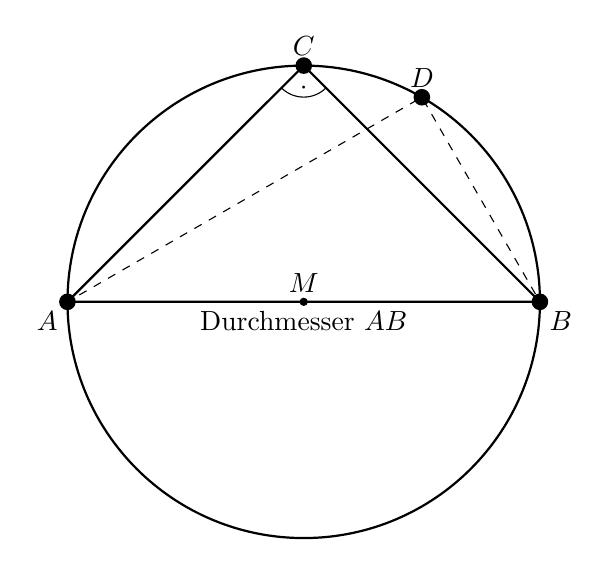
\begin{tikzpicture}[scale=1.5]

% Punkte A und B (Durchmesser)
\coordinate (A) at (0,0);
\coordinate (B) at (4,0);

% Mittelpunkt des Kreises
\coordinate (M) at ($(A)!0.5!(B)$);

% Kreis mit Durchmesser AB
\draw[thick] (M) circle ({0.5*veclen({4},{0})}); % Radius = AB/2

% Punkt C auf dem Kreis (frei wählbar)
\coordinate (C) at ($(M)+(0,2)$);
\coordinate (D) at ($(M)+({1},{sqrt(3)})$);

% Dreieck ABC
\draw[thick] (A) -- (B) -- (C) -- cycle;
\draw[dashed] (A) -- (B) -- (D) -- cycle;

% Punkte markieren
\fill (A) circle (2pt) node[below left] {$A$};
\fill (B) circle (2pt) node[below right] {$B$};
\fill (C) circle (2pt) node[above] {$C$};
\fill (M) circle (1pt) node[above] {$M$};
\fill (D) circle (2pt) node[above] {$D$};

% Rechter Winkel bei C (nur Viertelkreis)
\pic [draw, angle radius=0.4cm] {angle = A--C--B};

% Punkt in den Winkel setzen (klassisch deutsch)
\path (C) ++(270:0.19cm) node {$\cdot$};

% Beschriftung Durchmesser
\node[below] at ($(A)!0.5!(B)$) {Durchmesser $AB$};

\end{tikzpicture}
\end{center}
\end{theorem}
\newpage
\section{Analytische Geometrie/Lineare Algebra}

Nachdem wir uns mit der Mittelstufengeometrie vertraut gemacht haben, kommen wir zum Stoff, der in der Q12 erstmals behandelt wurde. Die Geometrie wurde hier um einen grundlegenden Begriff erweitert: Der Vektor. 

\subsection{Grundlagen der Vektorgeometrie}
\begin{definition}
Die Menge aller gleichlanger, zueinander paralleler und gleichgerichteter Pfeile nennt man \textbf{Vektor}\index{Vektor}. Man bezeichnet sie mit $\vv{v}$. Jeder Pfeil ist ein Repräsentant eines Vektors. \par
Im zweidimensionalen Koordinatensystem hat jeder Vektor $\vv{v}$ zwei Koordinaten, im Dreidimensionalen besitzt jeder Vektor drei Einträge. Man schreibt:
\[ \vv{v} = \begin{pmatrix}
x_1 \\ x_2
\end{pmatrix} \hspace{1cm} \text{bzw.} \hspace{1cm} \vv{v} = \begin{pmatrix}
x_1 \\ x_2 \\ x_3
\end{pmatrix} \]
Anstelle der Raumachsen $x_1, x_2, x_3$ nutzt man auch die Bezeichnungen $x,y,z$. Um zu zeigen, dass ein Vektor zwei Einträge hat, also zweidimensional ist, schreibt man auch $\R^2$, für dreidimensionale Vektoren nutzt man $\R^3$.
\end{definition}

\begin{example}
Die unten stehenden Repräsentanten sind alle Teil des gleichen Vektors, da sie dieselbe Richtung und die gleiche Länge haben. Sie sind also auch parallel.
\begin{center}
\begin{tikzpicture}
\draw[->]	(0,0) -- (2,1);
\draw[->]	(1,1) -- (3,2);
\draw[->]	(1,-1) -- (3,0);
\draw[->]	(2,0) -- (4,1);
\end{tikzpicture}
\end{center}
\end{example}

Ein wichtiger Zusammenhang besteht zwischen Punkten und Vektoren. Punkte haben feste Koordinaten, während sich Vektoren im Raum beliebig verschieben lassen. Ein spezieller Vektor, der in gewisser Weise die Verbindung von Punkt und Vektor herstellt, ist der Ortsvektor.

\begin{definition}
Sei $A(x_1|x_2|x_3)$ bzw. $B(x|y)$ ein Punkt. Dann heißt 
\[ \vv{OA} = \begin{pmatrix} x_1 \\ x_2 \\ x_3 \end{pmatrix} \hspace{1cm} \text{bzw.} \hspace{1cm} \vv{OB} \begin{pmatrix} x \\ y  \end{pmatrix} \]
\textbf{Ortsvektor}. Ein Repräsentant des Ortsvektors ist anschaulich der Pfeil vom Koordinatenursprung zum Punkt.
\index{Ortsvektor} \index{Vektor!Orts}
\end{definition}

\begin{example}
Gegeben sei der Punkt $A(1|2|-3)$. Dann heißt der dazugehörige Ortsvektor $\vv{OA}=\begin{pmatrix} 1 \\ 2 \\ -3 \end{pmatrix}$. Graphisch kann man ihn sich als Pfeil vom Ursprung zum Punkt $A$ vorstellen:
\begin{center}
\begin{tikzpicture}
\begin{axis}[
	axis lines = middle,
	view = {120}{20},
	xmin=0, xmax = 3,
	ymin=0, ymax = 3,
	zmin=-3, zmax=1,
    axis equal
]

\addplot3[->, thick, blue]	coordinates	{(0,0,0) (1,2,-3)}	node[pos=1, above right]	{$\vv{OA}$};

% Manuelle Achsenbeschriftung
\node at (axis cs:5,0,0) [anchor=west] {$x$};
\node at (axis cs:0,4.5,0) [anchor=south] {$y$};
\node at (axis cs:0,0,1.5) [anchor=north] {$z$};
\end{axis}
\end{tikzpicture}
\end{center}
Wir man leicht sehen kann, ist eine Zeichnung eines Vektors nicht immer eindeutig. Darauf sollte man also achten, wenn man mit Vektoren arbeitet.
\end{example}

\begin{theorem} \textbf{(Rechenregeln für Vektoren)}
\begin{enumerate}
\item Der Nullvektor ist derjenige Vektor, für den jeder Eintrag gleich $0$ ist. Er heißt $\vv{0}$.
\item Für beliebige Vektoren ist die Addition definiert als
\[ \vv{a} + \vv{b} = \begin{pmatrix} a_1+b_1 \\ a_2+b_2  \end{pmatrix} \hspace{1cm} \text{bzw.} \hspace{1cm}  \vv{a} + \vv{b} = \begin{pmatrix} a_1+b_1 \\ a_2+b_2 \\ a_3+b_3  \end{pmatrix} \]
Sie ist kommutativ. Es gilt also $\vv{a} + \vv{b} = \vv{b} + \vv{a}$.
\item Für eine beliebige reelle Zahl $\lambda \in \R$ gilt \[ \lambda \cdot \vv{a} = \lambda \cdot \begin{pmatrix} a_1 \\ a_2  \end{pmatrix} = \begin{pmatrix} \lambda \cdot a_1 \\ \lambda \cdot a_2  \end{pmatrix} \hspace{0.6cm} \text{bzw.} \hspace{0.6cm}  \lambda \cdot \vv{a} = \lambda \cdot \begin{pmatrix} a_1\\ a_2 \\ a_3 \end{pmatrix} = \begin{pmatrix} \lambda \cdot a_1\\ \lambda \cdot a_2 \\ \lambda \cdot a_3 \end{pmatrix}\]
Diese Operation heißt \textbf{skalare Multiplikation}.
\item Der Vektor $(-1)\cdot \vv{a} = -\vv{a}$ heißt \textbf{Gegenvektor} von $\vv{a}$.
\item Die Subtraktion $\vv{a} - \vv{b}$ wird definiert als $\vv{a} +  (-\vv{b})$. Auch sie ist also kommutativ.
\item Für beliebige reelle Zahlen $\lambda \in \R$ und jeden Vektor $\vv{a}$ gilt:
\[ 0 \cdot \vv{a} = \lambda \cdot \vv{0} = \vv{0} \]
\index{Rechenregeln für Vektoren} \index{Gegenvektor} \index{Vektoraddition}
\end{enumerate}
\label{Satz:RR_fuer_Vektoren}
\end{theorem}

\begin{example} \

\[  \mleft(\colvec[3]{6}{9} - 3 \cdot \colvec[1]{2}{3} \mright)   \cdot \pi^2 =  \colvec[3-3]{6-6}{9-9}  \cdot \pi^2 = \vv{0}\cdot \pi^2 = \vv{0} \]

\end{example}

Manchmal ist es praktisch, einen Vektor zu haben, der die Länge $1$ besitzt, aber die Richtung des urpsprüunglichen Vektors beibehält. Dafür definieren wir folgendes:

\begin{definition} \
\begin{enumerate}
\item Für den Betrag eines zweidimensionalen Vektors $\\v{a}=\colvec{a_1}{a_2}$ gilt:
\[ |\vv{a}| = \sqrt{a_1^2+a_2^2}\]
\item Für den Betrag eines dreidimensionalen Vektors $\\v{a}=\colvec[a_1]{a_2}{a_3}$ gilt:
\[ |\vv{a}| = \sqrt{a_1^2+a_2^2+a_3^2}\]
\item Der \textbf{Einheitsvektor} oder \textbf{Normierte Vektor} $\vv{a_0}$ eins Vektors $\vv{a}$ hat Länge $1$ und zeigt in die gleiche Richtung wie $\vv{a}$ selbst. Für ihn gilt:
\[ \vv{a_0} = \dfrac{1}{|\vv{a}|} \cdot \vv{a}\]
\end{enumerate}
\index{Einheitsvektor} \index{Normierter Vektor} \index{Vektor!normieren}
\end{definition}
Nun fragen wir uns, wie wir allgemeiner den Vektor zwischen zwei Punkten bestimmen können. Für einen beliebigen Punkt kennen wir den Ortsvektor. 

\begin{theorem}
Zwischen zwei Punkten $A$ und $B$ mit Ortsvektoren $\vv{OA}=\colvec[a_1]{a_2}{a_3}$ und $\vv{OB}=\colvec[b_1]{b_2}{b_3}$ ermittelt man den Vektor von $A$ nach $B$ wiefolgt:
\[ \vv{AB}=\vv{OB} - \vv{OA} = \colvec[b_1-a_1]{b_2-a_2}{b_3-a_3} \]
Ein Merkspruch lautet \glqq Hinten minus vorne.\grqq
\end{theorem}

\begin{example}
Nun sind die Punkte $A(2|0|1)$ und $B(0|1|1)$ gegeben. Wir möchten den Vektor $\vv{AB}$ ermitteln. Rechnerisch gilt hierbei:
\[  \vv{AB} = \vv{OB} - \vv{OA} = \colvec[0]{1}{1} - \colvec[2]{0}{1} = \colvec[-2]{1}{0}  \]
Graphisch sieht das wiefolgt aus:
\begin{center}
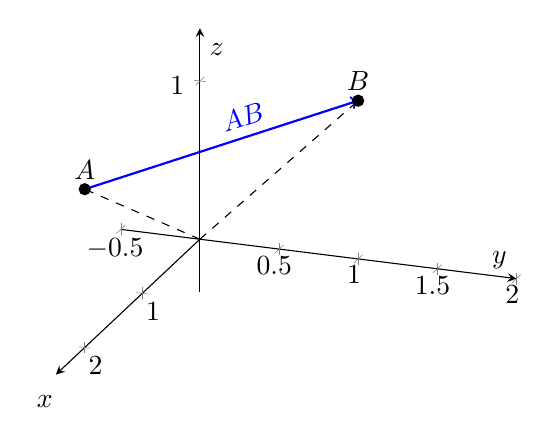
\begin{tikzpicture}
\begin{axis}[
    axis lines = middle,
    view = {110}{20},
    xmin=0, xmax=2.5,
    ymin=0, ymax=1.5,
    zmin=0, zmax=1,
    axis equal,
]

% Punkte A und B
\addplot3[only marks, mark=*] coordinates {(2,0,1)};
\addplot3[only marks, mark=*] coordinates {(0,1,1)};

\node at (axis cs:2,0,1) [above] {$A$};
\node at (axis cs:0,1,1) [above]  {$B$};

% Ortsvektor OA (gestrichelt)
\addplot3[dashed]
coordinates {(0,0,0) (2,0,1)};

% Ortsvektor OB (gestrichelt)
\addplot3[dashed]
coordinates {(0,0,0) (0,1,1)};

% Vektor AB (blau, fett)
\addplot3[->, thick, blue]
coordinates {(2,0,1) (0,1,1)}
node[pos=0.6, above, sloped] {$\vv{AB}$};

% Manuelle Achsenbeschriftung
\node at (axis cs:3,0,0) [anchor=west] {$x$};
\node at (axis cs:0,2,0) [anchor=south east] {$y$};
\node at (axis cs:0,0,1.2) [anchor=west] {$z$};

\end{axis}
\end{tikzpicture}
\end{center}
\end{example}

In Satz \ref{Satz:RR_fuer_Vektoren} haben wir bereits die skalare Multiplikation kennengelernt. Skalare sind dabei reelle Zahlen. Das Skalarprodukt heißt so, weil es eine reelle Zahl als Ergebnis ausgibt, also einen Skalar.

\begin{definition}
Für die Vektoren $\vv{a},\vv{b}\neq \vv{0}$ nennen wir die reelle Zahl
\[ \vv{a} \circ \vv{b} = |\vv{a}|\cdot |\vv{b}| \cdot \cos \varphi \]
\textbf{Skalarprodukt} von $\vv{a}$ und $\vv{b}$. Im $\R^2$ gilt:
\[ \vv{a} \circ \vv{b}=|\vv{a}| \cdot |\vv{b}| \cdot \cos (\varphi) = a_1\cdot b_1 + a_2 \cdot b_2 \]
Analog dazu gilt im dreidimensionalen $\R^3$:
\[ \vv{a} \circ \vv{b}=|\vv{a}| \cdot |\vv{b}| \cdot \cos (\varphi) = a_1\cdot b_1 + a_2 \cdot b_2 + a_3 \cdot b_3 \]
\index{Skalarprodukt}
\end{definition}

\begin{theorem} Die Vektoren $\vv{a},\vv{b}\neq \vv{0}$ sind \textbf{genau dann} orthogonal zueinander, wenn gilt: $\vv{a} \circ \vv{b} = 0$. \par
Orthogonal\index{Orthogonal} heißt senkrecht\index{Senkrecht} zueinander; Die Vektoren schließen also einen $\ang{90}$-Winkel ein, wenn sie orthogonal zueinander stehen.
\end{theorem}

\begin{example}
Wir betrachten nun die Vektoren $\vv{a}=\colvec{2}{1}, \vv{b}=\colvec{1}{-2}$ und $\vv{c}=\colvec{-3}{1}$.
Für die Skalarprodukte gilt:
\begin{enumerate}
\item $\vv{a} \circ \vv{b} = 2\cdot 1 + 1 \cdot (-2) = 0 \Rightarrow$ Die Vektoren sind orthogonal zueinander.
\item $\vv{b} \circ \vv{c} = 1 \cdot (-3) + (-2) \cdot 1 = -5 \neq 0 \Rightarrow$ Die Vektoren schließen einen Winkel ein, der nicht $\ang{90}$ beträgt. Wir nutzen aus, dass
\[ -5 = |\vv{b}| \cdot |\vv{c}| \cdot \cos (\varphi)\]
gilt. Denn so können wir den Winkel bestimmen:
\[ -5 = \sqrt{1^2+(-2)^2} \cdot \sqrt{(-3)^2+1^2} \cdot \cos (\varphi) \Rightarrow \varphi = \cos^{-1} \mleft( \dfrac{-5}{\sqrt{5}\cdot \sqrt{10}} \mright) = \ang{135}\]
\item Der Schnittwinkel für $\vv{a}$ und $\vv{c}$ beträgt ebenfalls $\ang{135}$. (Übung)
\end{enumerate}
\end{example}

Im $\R^3$ gibt es noch ein besonderes \glqq Produkt\grqq , nämlich das Kreuzprodukt.

\begin{definition}
Für die Vektoren $\vv{a}=\colvec[a_1]{a_2}{a_3}$ und $\vv{b}=\colvec[b_1]{b_2}{b_3}$ definiert man das \textbf{Kreuzprodukt}\index{Kreuzprodukt} oder Vektorprodukt \index{Vektorprodukt} als
\[ \vv{a} \times \vv{b} = \colvec[a_2\cdot b_3-a_3\cdot b_2]{a_3\cdot b_1-a_1\cdot b_3}{a_1\cdot b_2 - a_2 \cdot b_1}.\]
\end{definition}

Das Kreuzprodukt ist nützlich, da es uns stets einen dritten Vektor liefert, der orthogonal zu $\vv{a}$ und $\vv{b}$ ist. Dies kann man durch Anwenden des Skalarproduktes nachrechnen (Übung). Wir fassen diese Erkenntnis im folgenden Satz zusammen:

\begin{theorem}
Ist das Kreuzprodukt $\vv{a}\times \vv{b}$ vom Nullvektor verschieden, so ist der Vektor $\vv{c}=(\vv{a}\times \vv{b})$ orthogonal zu $\vv{a}$ und $\vv{b}$.
\end{theorem}

\begin{example}
Für die Vektoren $\vv{a}=\colvec[1]{2}{3}$ und $\vv{b}=\colvec[4]{5}{6}$ erhalten wir das Kreuzprodukt durch
\[ \vv{a}\times \vv{b} = \colvec[2\cdot 6 - 3 \cdot 5]{3 \cdot 4 - 1 \cdot 6}{1\cdot 5 - 2 \cdot 4} = \colvec[-3]{6}{-3}  \]
Tatsächlich ist der so entstandene Vektor orthogonal zu $\vv{a}$ und $\vv{b}$ (Übung). 
\end{example}

Oft nutzt man das Kreuzprodukt aber nicht nur, um einen senkrechten Vektor zu erhalten, sondern um Flächen und Volumina zu berechnen. 

\begin{theorem} \ 
\begin{enumerate}
\item Der Flächeninhalt des Parallelogramms, das von den Vektoren $\vv{a},\vv{b}\neq \vv{0}$ unter dem Winkel $\varphi$ aufgespannt werden, beträgt
\[ A_{\mathrm{Parallelogramm}} = |\vv{a}\times \vv{b}| = |\vv{a}| \cdot |\vv{b}| \cdot \sin \varphi . \]
\index{Flächeninhalt!eines Parallelogramms mithilfe des Kreuzprodukts}
\item Für ein Dreieck mit zwei Seiten, die von den Vektoren $\vv{a}$ und $\vv{b}$ begrenzt werden, gilt $A=\dfrac{1}{2}\cdot \mleft| \vv{a} \times \vv{b} \mright|$.
\item Das Volumen des Spates, der von den Vektoren $\vv{a},\vv{b}, \vv{c} \neq \vv{0}$ aufgespannt wird, beträgt
\[ V_{\mathrm{Spat}} = \mleft| \mleft( \vv{a}\times \vv{b} \mright) \circ \vv{c} \mright| \]
Der Ausdruck $\mleft| \mleft( \vv{a}\times \vv{b} \mright) \circ \vv{c} \mright|$ heißt \textbf{Spatprodukt}. \index{Spatprodukt} \index{Volumen!eines Spats}
\item Für eine Pyramide mit viereckiger Grundfläche gilt:
\[ V_{\mathrm{Pyramide}} = \dfrac{1}{3} \mleft| \mleft( \vv{a}\times \vv{b} \mright) \circ \vv{c} \mright| \] \index{Volumen!einer Pyramide}
\item Für Pyramiden mit dreieckiger Grundfläche (Tetraeder) gilt:
\[ V_{\mathrm{Tetraeder}} =\dfrac{1}{6} \mleft| \mleft( \vv{a}\times \vv{b} \mright) \circ \vv{c} \mright| \] \index{Volumen!eines Tetraeders}
\end{enumerate}
\end{theorem}

\begin{example}
Gegeben sind die Vektoren $\vv{a}=\colvec[1]{-\num{1,5}}{0}$ und $\vv{b}=\colvec[2]{2}{0}$. Das Kreuzprodukt der beiden Vektoren lautet rechnerisch nun
\[ \vv{a} \times \vv{b} = \colvec[(1\cdot 0) - (0 \cdot 2)]{(0\cdot 2) - (1 \cdot 0)}{(1\cdot 2) - (-\num{1,5} \cdot 2)} = \colvec[0]{0}{5}\]
Graphisch sehen die drei Vektoren im Verhältnis wiefolgt aus, wenn man $(\vv{a}\times \vv{b})$ als Vektor $\vv{c}$ bezeichnet:
\begin{center}
\begin{tikzpicture}
\begin{axis}[
    axis lines = middle,
    view = {110}{20},
    xmin=-4.5, xmax=4.5,
    ymin=-4.5, ymax=5.5,
    zmin=0, zmax=5.5,
    axis equal,
    ticks=none,
]



% Ortsvektor OA (gestrichelt)
\addplot3[->, thick, black]
coordinates {(0,0,0) (1,-1.5,0)}
node[pos=0.6, above, sloped] {$\vv{a}$};
% Ortsvektor OB (gestrichelt)
\addplot3[->, thick, red]
coordinates {(0,0,0) (2,2,0)}
node[pos=0.6, above, sloped] {$\vv{b}$};
% Vektor AB (blau, fett)
\addplot3[->, thick, blue]
coordinates {(0,0,0) (0,0,5)}
node[pos=0.6, above, sloped] {$\vv{c}$};

% Manuelle Achsenbeschriftung
\node at (axis cs:5.2,0,0) [anchor=west] {$x$};
\node at (axis cs:0,6,0) [anchor=south east] {$y$};
\node at (axis cs:0,0,6) [anchor=west] {$z$};

\end{axis}
\end{tikzpicture}
\end{center}
Wir sehen also, dass der Vektor $\vv{c}$ offensichtlich im rechten Winkel zu den anderen beiden Vektoren steht. 
\end{example}

\newpage 

\subsection{Geraden und Ebenen im Raum}

Nachdem wir uns in Jahrgangsstufe 12 mit den Vektoren vertraut gemacht haben, folgten in Jahrgangsstufe 13 die Nutzung der Vektoren in Geraden und Ebenen. Ein grundlegendes Konzept, das man für Vektoren, speziell in Ebenen und Geraden, oft benötigt, ist die lineare Unabhängigkeit.

\begin{definition}
Eine \textbf{Linearkombination} der Vektoren $\vv{v_1}, \vv{v_2}, \ldots, \vv{v_n}$ ist ein Vektor der Form
\[ \sum_{k=1}^n \lambda_k \vv{v_k} = \lambda_1 \cdot \vv{v_1} + \lambda_2 \cdot \vv{v_2} + \ldots + \lambda_n \cdot \vv{v_n} \hspace{0.5cm} \text{mit} \hspace{0.5cm} \lambda_1,\ldots ,\lambda_n \in \R . \]
\index{Linearkombination}
\end{definition}

\begin{example} \
\begin{enumerate}
\item Für die Vektoren $\vv{a}=\colvec[1]{0}{0}, \vv{b}=\colvec[0]{1}{0}$ und $\vv{c}=\colvec[0]{0}{1}$ lässt sich der Vektor $\vv{v_1}=\colvec[1]{2}{5}$ als Linearkombination darstellen, denn
\[ \colvec[1]{2}{5} = 1\cdot \colvec[1]{0}{0} + 2\cdot \colvec[0]{1}{0} + 5 \cdot \colvec[0]{0}{1}\]
\item Auch der Vektor $\vv{v_2}=\colvec[4]{-3}{2}$ ist als Linearkombination von $\vv{a}, \vv{b}$ und $\vv{c}$ darstellbar:
\[ \colvec[4]{-3}{2} = 4 \cdot \vv{a} + (-3) \cdot \vv{b} + 2 \cdot \vv{2}  \]
\end{enumerate}
\label{Bsp:LinKomb}
\end{example}

\begin{theorem} \textbf{(Satz über lineare Unabhängigkeit)} \par
Gegeben sind die Vektoren $\vv{v_1}, \vv{v_2}, \ldots, \vv{v_n}$. Die folgenden Aussagen sind äquivalent:
\begin{enumerate}[i)]
\item Die Vektoren $\vv{v_1}, \vv{v_2}, \ldots, \vv{v_n}$ sind \textbf{linear unabhängig}. \index{Lineare Unabhängigkeit}
\item Man kann keinen Vektor $\vv{v_1}, \vv{v_2}, \ldots, \vv{v_n}$ als Linearkombination der \textbf{anderen} Vektoren aus $\vv{v_1}, \vv{v_2}, \ldots, \vv{v_n}$ darstellen.
\item Der Nullvektor $\vv{0}$ lässt sich nur trivial als Linearkombination der Vektoren $\vv{v_1}, \vv{v_2}, \ldots, \vv{v_n}$ darstellen, d.h. für $\lambda_i \in \R$ gilt:
\[ \lambda_1 \cdot \vv{v_1} + \lambda_2 \cdot \vv{v_2} + \ldots + \lambda_n \cdot \vv{v_n} \Rightarrow \lambda_1 = \lambda_2 = \ldots = \lambda_n=0  \]
\end{enumerate}
\label{Satz:LinUnabh}
Ansonsten heißen die Vektoren $\vv{v_1}, \vv{v_2}, \ldots, \vv{v_n}$ \textbf{linear abhängig}.
\end{theorem}

Eine kleine Anmerkung lässt sich hier nicht vermeiden. Die Bezeichnung \emph{trivial} bedeutet in der Mathematik, dass etwas offensichtlich ist. In diesem Fall ist die triviale Darstellung des Nullvektors die, bei der alle Vorfaktoren $\lambda_1 = \ldots = \lambda_n=0$ gesetzt werden. \glqq Trivialerweise\grqq \ oder offensichtlich gilt nämlich
\[ 0\cdot \colvec[1]{2}{300} + 0 \cdot \colvec[2]{-40}{\pi} + 0 \cdot \colvec[4]{2}{1} = \colvec[0]{0}{0} = \vv{0}\]
Das gilt natürlich für beliebig viele Vektoren mit beliebigen Einträgen, solange die Vorfaktoren immer gleich $0$ bleiben. Die lineare Unabhängigkeit betrachten wir nun anhand eines Beispiels, in dem wir die beiden Varianten aus Satz \ref{Satz:LinUnabh} ii) und iii) nutzen:

\begin{example}
Wir betrachten erneut die Vektoren aus Beispiel \ref{Bsp:LinKomb}. Die drei Vektoren $\vv{a}=\colvec[1]{0}{0}, \vv{b}=\colvec[0]{1}{0}$ und $\vv{c}=\colvec[0]{0}{1}$ sind linear unabhängig. Beispielsweise kann man versuchen, den Nullvektor zu erzeugen und erhält so ein lineares Gleichungssystem:
\[ \colvec[0]{0}{0} \overset{!}{=} \lambda_1 \cdot \colvec[1]{0}{0} + \lambda_2 \cdot \colvec[0]{1}{0} + \lambda_3 \cdot \colvec[0]{0}{0} \]
\[ \Rightarrow \colvec[0]{0}{0} \stackrel{!}{=} \colvec[\lambda_1]{\lambda_2}{\lambda_3} \Rightarrow \lambda_1 = \lambda_2 = \lambda_3 = 0\]
Nach Satz \ref{Satz:LinUnabh} iii) sind die Vektoren $\vv{a}, \vv{b}$ und $\vv{c}$ linear unabhängig. \par
Betrachten wir die Vektoren $\vv{a}, \vv{v_2}$ und den neuen Vektor $\vv{v_3}=\colvec[5]{3}{-2}$, so sind diese \textbf{linear abhängig}. Nutzen wir beispielsweise Satz \ref{Satz:LinUnabh} ii), so schreiben wir $\vv{v_2}$ als
\[ \colvec[4]{-3}{2} = -1\cdot \colvec[5]{3}{-2} + 9 \cdot \colvec[1]{0}{0}   \]
Da sich ein Vektor als Linearkombination der anderen Vektoren darstellen lässt, sind die drei Vektoren $\vv{a}, \vv{v_2}$ und $\vv{v_3}$ linear abhängig. \par
Würden wir beispielsweise den Vektor $\vv{a}$ weglassen, so wären die zwei Vektoren wieder linear unabhängig. (Übung)
\end{example}

Nun gehen wir zum wirklich interessanten Teil über, den Geraden und Ebenen. Dabei definiert man Geraden wiefolgt:

\begin{definition}
Jede Gerade\index{Gerade!im Dreimimensionalen} ist darstellbar in der Form
\[ g:\vv{x}=\vv{OA}+\lambda\cdot \vv{u} \ (\lambda \in \R, \vv{u} \neq \vv{0})  \]
Dabei stellt $\vv{x}$ einen Ortsvektor eines beliebigen Punktes auf der Geraden dar. Jeder Punkt, dessen Ortsvektor also diese Gleichung erfüllt, liegt auf der Geraden. \par
Diese Art der Darstellung heißt \textbf{Parameterform} \index{Parameterform!einer Geraden} mit dem \textbf{Aufpunkt} $A$ und dem \textbf{Richtungsvektor} $\vv{u}$. $\vv{OA}$ nennt man dabei \textbf{Stützvektor}.
\begin{center}
\begin{tikzpicture}
\begin{axis}[
    axis lines = middle,
    view = {115}{12},   % flacherer Blickwinkel
    xmin=-3, xmax=5,
    ymin=-3, ymax=5,
    zmin=-3, zmax=3,
    axis equal,
    ticks=none,
]

% Punkt A
\addplot3[only marks, mark=*, mark size=2.5pt] 
coordinates {(1,1,1)};
\node at (axis cs:1,1,1) [above] {$\vv{OA}$};

% Stützvektor OA
\addplot3[->, thick]
coordinates {(0,0,0) (1,1,1)}
node[pos=0.6, below left] {};



% komplette Gerade g
\addplot3[
    domain=-3:3,
    samples=2,
    dashed,
    black
]
({1 - 3*x},
 {1 + 1*x},
 {1 + 0*x});

\node at (axis cs:4,0,1.8) {$g$};

% Richtungsvektor u (farbig)
\addplot3[->, thick, red]
coordinates {(1,1,1) (-2,2,1)}
node[pos=0.6, above] {$\vv{u}$};

\end{axis}
\end{tikzpicture}
\end{center}
\end{definition}

\begin{example}
Für die Gerade $g:\vv{x}=\colvec[0]{0}{1}+\lambda \cdot \colvec[1]{1}{0}$ prüfen wir, ob der Punkt $B$ mit Ortsvektor $\vv{OB}=\colvec[4]{4}{1}$ auf der Geraden liegt. Dazu setzen wir in die Geradengleichung ein:
\[ \colvec[4]{4}{1} \stackrel{!}{=} \colvec[0]{0}{1} + \lambda \cdot \colvec[1]{1}{0} \]
Hieraus erhalten wir drei lineare Gleichungen, die wir nun nach $\lambda$ auflösen. Falls $\lambda$ in allen Fällen die Lösung ist, liegt $B$ auf der Geraden.
\begin{align*}
\mathrm{(I)}\quad	&	0 + \lambda \cdot 1 = 4 \\
\mathrm{(II)}\quad	&	0 + \lambda \cdot 1 = 4 \\
\mathrm{(III)}\quad	&	1 + \lambda \cdot 0 = 1
\end{align*}
Für $\mathrm{(I)}$ und $\mathrm{(II)}$ erhalten wir die Lösung $\lambda = 4$, und in $\mathrm{(III)}$ ist $\lambda=4$ auch eine Lösung, denn $1+ 0 \cdot 4 = 1$. Da wir $B$ nun also in der Geradengleichung angeben können, liegt $B$ auf der Geraden.
\end{example}

\begin{theorem} \textbf{(Bestimmung einer Geradengleichung)} \par
Sind die Punkte $A$ und $B$ gegeben, existiert eine Gerade durch die beiden Punkte. Man erhält sie wiefolgt:
\begin{enumerate}
\item Man wählt einen Punkt als Aufpunkt. Dessen Ortsvektor wird zum Stützvektor.
\item Der Vektor $\vv{u}=\vv{OA}-\vv{OB}$ wird zum Richtungsvektor.
\end{enumerate}
Die Reihenfolge, wie man $\vv{u}$ berechnet, ist egal, denn $\vv{OB}-\vv{OA}=-\vv{u}$. Der Vektor zeigt also in die andere Richtung, doch die Gerade erstreckt sich in beide Richtungen, weshalb das Vorzeichen von $\vv{u}$ keine Rolle spielt.
\end{theorem}

\begin{example}
Gegeben sind die Punkte $A(1|3|-3)$ und $B(2|-1|2)$. 
\begin{enumerate} [i)]
\item Wählen wir $A$ als Aufpunkt. Nun suchen wir einen Richtungsvektor $\vv{u}$, indem wir $\vv{OA}-\vv{OB}$ bestimmen:
\[ \vv{u}= \colvec[1]{3}{-3}-\colvec[2]{-1}{2} = \colvec[-1]{4}{-5}\]
Die Geradengleichung können wir also angeben als 
\[ g:\vv{x} = \colvec[1]{3}{-3}+\lambda \colvec[-1]{4}{-5}\]
\item Nehmen wir nun $B$ als Aufpunkt. Als Richtungsvektor rechnen wir exemplarisch $\vv{OB}-\vv{OA}$, aber auch hier ist der Richtungsvektor aus i) denkbar. Wir erhalten jedenfalls:
\[ \colvec[2]{-1}{2} - \colvec[1]{3}{-3} = \colvec[1]{-4}{5} = -\vv{u}\]
Die Geradengleichung lautet hier also
\[ g':\vv{x} = \colvec[2]{-1}{2} + \lambda \colvec[1]{-4}{5}\]
\end{enumerate}
Doch wie kann es sein, dass wir scheinbar zwei völlig verschiedene Ausdrücke haben, wo doch beide die Gerade durch $A$ und $B$ angeben? Tatsächlich können wir die eine Geradengleichung in die andere überführen. \par
Wir dürfen jeden beliebigen Punkt der Geraden als Aufpunkt nehmen. Und wir wissen, dass beim Vektor nur die Richtung relevant ist, nicht aber die Länge oder ob er \glqq vorwärts\grqq \ (zum Beispiel $\vv{u}$) bzw. \glqq rückwärts\grqq \ ($-\vv{u}$) ausgerichtet ist. Mathematisch präziser lässt sich formulieren, dass man jeden \textbf{parallelen} Vektor zu $\vv{u}$ als Richtungsvektor nutzen kann. Diese zwei Erkenntnisse nutzen wir nun, um uns von der Gleichheit der Geraden zu überzeugen. \par
Dass die beiden Richtungsvektoren parallel sind, haben wir bereits herausgefunden, also bleibt nur noch zu zeigen, dass der Aufpunkt der einen Geraden in der anderen Geraden enthalten ist. Wählen wir den Aufpunkt $A$ der Geraden $g$, so prüfen wir, ob $A\in g'$ ist, indem wir den Ortsvektor von $A$ in die Geradengleichung $g'$ einsetzen:
\[ \vv{OA} = \colvec[1]{3}{-3} \stackrel{!}{=} \colvec[2]{-1}{2} + \lambda \colvec[1]{-4}{5}\]
Wir erhalten den Parameter $\lambda=-1$ als Lösung der Gleichungen. (Übung) \par
Nun sind wir sicher: Die Geradengleichung $g'$ ist eine andere Schreibweise für $g$. Es gilt $g'=g$
\label{Bsp:GeradenGleichung}
\end{example}

Was wir in diesem Beispiel bereits angerissen haben ist die gegenseitige Lagebeziehung zweier Geraden. Die verschiedenen Arten, wie Geraden zueinander liegen können, listen wir dafür im nächsten Satz auf und liefern dazu auch Kriterien zum Überprüfen mit.

\begin{theorem} \textbf{(Lagebeziehung zweier Geraden) \index{Gerade!Lagebeziehungen zweier}} \par
Seien $g:\vv{x}=\vv{OA}+\lambda_1 \cdot \vv{u}$ und $h:\vv{x}=\vv{OB}+\lambda_2 \cdot \vv{v}$ zwei Geraden. Dann gilt für ihre Lagebeziehung:
\begin{enumerate}
\item Sind $\vv{u}$ und $\vv{v}$ \textbf{linear abhängig}, so sind $g$ und $h$ \textbf{parallel} zueinander. \index{Gerade!parallel}
\item Gilt zusätzlich zu 1., dass $A$ auf $h$ liegt, so sind $g$ und $h$ identisch.
\item Falls $A$ nicht auf $h$ liegt, nennt man $g$ und $h$ \textbf{echt parallel}.
\item Sind $g$ und $h$ nicht parallel und besitzt $\vv{OA}+\lambda_1 \vv{u} = \vv{OB}\cdot \lambda_2\vv{v}$ keine Lösung, so sind $g$ und $h$ zueinander \textbf{windschief}. \index{Gerade!windschief}
\item Existiert eine Lösung, haben $g$ und $h$ also einen Punkt gemeinsam, so schneiden sich $g$ und $h$ in einem Punkt. \index{Gerade!Schnittpunkt}
\end{enumerate}
\end{theorem}

\begin{example}
Wir wollen für jeden der Fälle ein konkretes Beispiel betrachten.
\begin{enumerate}
\item Aus Beispiel \ref{Bsp:GeradenGleichung} kennen wir bereits den Fall, dass $g$ und $h$ \textbf{identisch} sind.
\item Seien $g:\vv{x}=\colvec[4]{0}{0} + \lambda \colvec[1]{4}{-3}$ und $h:\vv{x}=\colvec[7]{8}{-6} + \mu \colvec[-2]{-8}{6}$ zwei Geraden. Zuerst prüfen wir, ob die Richtungsvektoren $\vv{u}$ und $\vv{v}$ parallel zueinander sind. Das ist genau dann der Fall, wenn die beiden Vektoren linear abhängig sind. Das bedeutet, wir können $\vv{v}$ als Vielfaches von $\vv{u}$ ausdrücken. Dazu stellen wir das folgende Gleichungssystem auf:
\begin{align*}
\mathrm{(I)} \quad & -2 = \lambda \cdot 1 \\
\mathrm{(II)} \quad & -8 = \lambda \cdot 4 \\
\mathrm{(III)} \quad & 6 = \lambda \cdot -3
\end{align*}
Daraus erhalten wir die Lösungen
\begin{align*}
\mathrm{(I)} \quad & \lambda = -2 \\
\mathrm{(II)} \quad & \lambda = -2 \\
\mathrm{(III)} \quad & \lambda = -2 \\
\end{align*}
Unsere Variable $\lambda$ ist also in allen drei Gleichungen identisch. Daraus folgt, dass $g$ und $h$ parallel sind. Nun gilt es zu überprüfen, ob sie echt parallel oder identisch sind. Dazu setzen wir den Aufpunkt von $h$ in $g$ ein:
\[ \colvec[7]{8}{-6} \stackrel{!}{=} \colvec[4+\lambda \cdot 1]{0 + \lambda \cdot 4}{0 - 3\cdot \lambda}  \]
Durch Rechnung entdecken wir, dass die Variable $\lambda$ bei den drei Gleichungen nicht gleich ist. (Übung) Wir stellen also fest, dass $g$ und $h$ nicht identisch, also \textbf{echt parallel} sind.
\item Gegeben sind nun die Geraden $g:\vv{x}=\colvec[2]{1}{-4} + \lambda \colvec[2]{-2}{0}$ und $h:\vv{x}=\colvec[9]{0}{-1} + \mu \colvec[3]{3}{3}$. Durch Rechnung oder geschicktes hinsehen stellt man fest, dass die Richtungsvektoren nicht parallel sind. Deshalb prüfen wir, ob ein Schnittpunkt existiert. Wir setzen die Geraden gleich:
\[ \colvec[2]{1}{-4} + \lambda \colvec[2]{-2}{0} = \colvec[9]{0}{-1} + \mu \colvec[3]{3}{3}  \Leftrightarrow \colvec[7]{-1}{3} = \colvec[2\lambda - 3\mu]{-2\lambda - 3 \mu}{-3\mu}\]
Daraus erhalten wir drei Gleichungssysteme mit zwei Unbekannten. Wir lösen das Gleichungssystem beispielsweise wiefolgt:
\begin{align*}
\mathrm{(I)} \quad & 7 = 2 \lambda - 3 \mu \\
\mathrm{(II)} \quad & -1 = -2 \lambda - 3 \mu \\
\mathrm{(III)} \quad & 3 = -3 \mu \\
\end{align*}
(III) liefert uns direkt $\mu = -1$. (III) in (II) ergibt $-1 = -2\lambda - (-3) \Rightarrow \lambda = 2$. Nun machen wir die Probe, indem wir beide Werte in (I) einsetzen: $7 = 2 \cdot 2 - (-3)$. Die Rechnung geht auf, wir haben einen Schnittpunkt! Um den Schnittpunkt $S$ zu bestimmen, setzen wir den ermittelten Wert von $\lambda$ oder von $\mu$ in die jeweilige Gerade ein. Zur Veranschaulichung, dass beide Male der gleiche Punkt herauskommt, prüfen wir exemplarisch beide Punkte:
\[ g: \vv{OS} = \colvec[2]{1}{-4} + 2 \cdot \colvec[2]{-2}{0} = \colvec[6]{-3}{-4} \]
\[ h: \vv{OS} = \colvec[9]{0}{-1} - 1 \cdot \colvec[3]{3}{3} = \colvec[6]{-3}{-4} \]
Wir sehen: Der Schnittpunkt hat die Koordinaten $S(6|-3|-4)$.
\item Greifen wir die Geraden aus 3. auf, wobei wir den Aufpunkt von $h$ ändern, sodass die neue Geradengleichung $h':\vv{x}=\colvec[9]{1}{-1} + \mu \colvec[3]{3}{3}$ lautet, ergibt sich wieder ein Gleichungssystem zur Überprüfung des Schnittpunktes. Diesmal lautet es
\begin{align*}
\mathrm{(I)} \quad & 7 = 2 \lambda - 3 \mu \\
\mathrm{(II)} \quad & 0 = -2 \lambda - 3 \mu \\
\mathrm{(III)} \quad & 3 = -3 \mu \\
\end{align*}
Hier lautet die Lösung aus (III) wiedermals $\mu = -1$. Das Einsetzen in (II) ergibt $\lambda=\frac{3}{2}$. Die Probe in (I) ergibt die Gleichung
\[ 2 \cdot \frac{3}{2} - (-3) = 3 + 3 = 6 \neq 7\]
Hier erhalten wir also keine Lösung, weshalb die Geraden $g$ und $h'$ keinen Schnittpunkt haben.
\end{enumerate}
\end{example}
Nachdem wir uns mit Geraden vertraut gemacht haben, blicken wir nun auf eine ganze Ebene. Während Geraden eindimensional sind (sie haben nur eine Richtung), sind Ebenen so etwas wie Flächen, also zweidimensional.

\begin{definition}
Ein Normalenvektor $\vv{n}$ \index{Normalenvektor} ist ein Vektor, der senkrecht (orthogonal; im $\ang{90}$-Winkel) auf einer Geraden, Ebene oder Fläche steht.
\end{definition}

\begin{definition} \index{Ebene!Darstellungen}
Eine Ebene ist ein zweidimensionales flaches Objekt. Wir beschreiben es mithilfe drei verschiedener Darstellungsarten:
\begin{enumerate}
\item \textbf{Parameterform:} Sei $A$ ein beliebiger Punkt in der Ebene und $\vv{u}$ und $\vv{v}$ zwei linear unabhängige Vektoren. Dann erfüllt der Ortsvektor eines jeden Punktes $X$, der in der Ebene liegt, die Gleichung
\[ E:\vv{x}=\vv{OA}+\lambda \vv{u} + \mu \cdot \vv{u} \]
Dabei heißt $A$ \textbf{Aufpunkt} und $\vv{u}$ und $\vv{v}$ heißen \textbf{Richtungsvektoren}.

\end{enumerate}
Sei $\vv{n}=\colvec[n_1]{n_2}{n_3}$ ein Normalenvektor und $A(a_1|a_2|a_3)$ ein Aufpunkt der Ebene. 
\begin{enumerate}[resume]
\item \textbf{Normalenform:} Jeder Punkt $X$ mit Ortsvektor $\vv{x}$, der in der Ebene $E$ liegt, erfüllt die Gleichung
\[ E:\vv{n}\circ \mleft( \vv{x} - \vv{OA} \mright) = 0  \]
\item \textbf{Koordinatenform:} Der Punkt $X(x_1|x_2|x_3)$ liegt in der Ebene, wenn die Gleichung
\[ E:n_1x_1+n_2x_2+n_3x_3 + k = 0 \hspace{1cm} \text{mit} \hspace{1cm} k = -(n_1a_1+n_2a_2+n_3a_3)\]
erfüllt ist.
\end{enumerate}
\begin{center}
\begin{tikzpicture}[scale=1.5, tdplot_main_coords]

  % Ebene als Parallelogramm
  \filldraw[fill=definitionblue!40, draw=definitionblue!40]
    (2,-1,1) -- (2,3,1) -- (-3,3,1) -- (-2,-1,1) -- cycle;

  % Koordinatenachsen
  \draw[->] (0,0,0) -- (3,0,0) node[below left] {$x$};
  \draw[->] (0,0,0) -- (0,3,0) node[below right] {$y$};
  \draw[->] (0,0,0) -- (0,0,3) node[left] {$z$};

  % Aufpunkt A = (-1,1,1)
  \coordinate (A) at (-1,1,1);
  \coordinate (O) at (0,0,0);

  % Richtungsvektoren e_1=(1,0,0), e_2=(0,1,0)
  % Parallelogramm-Punkte
  \coordinate (B) at ($(A)+(1,0,0)$); % A + e1
  \coordinate (C) at ($(A)+(1,1,0)$); % A + e1 + e2
  \coordinate (D) at ($(A)+(0,1,0)$); % A + e2

  


  % Aufpunkt markieren
 % \fill (A) circle (1pt) node[above left] {$A(-1,1,1)$};

  % Richtungsvektoren einzeichnen
  \draw[->, thick, purple] (A) -- (B) node[midway, right] {$\vv{v}$};
  \draw[->, thick, purple] (A) -- (D) node[midway, above] {$\vv{u}$};
  \draw[->, thick] (O) node[right=1.1cm, above=2pt] {$\vv{OA}$} -- (A);
  
  \draw[->, thick, blue] (A) -- ($(A)+(0,0,1)$) node[midway, left] {$\vv{n}$};

\end{tikzpicture}
\end{center}
\end{definition}

\begin{example} \
\begin{enumerate}
\item Gegeben sei zuerst der Richtungsvektor $\vv{u}=\colvec[1]{0}{0}$ und $\vv{v}=\colvec[0]{-1}{0}$ sowie der Aufpunkt $A(1|1|0)$. Bevor wir eine Ebenengleichung aufstellen, müssen wir zuerst die lineare Unabhängigkeit prüfen. Da die beiden Vektoren nicht parallel sind, sind sie linear unabhängig. (Übung) Die Ebenengleichung lautet
\[ E:\vv{x} = \colvec[1]{1}{0} + \lambda \cdot \colvec[1]{0}{0} + \mu \cdot \colvec[0]{-1}{0}\]
Sollen wir nun prüfen, ob ein Punkt $B(3|2|0)$ in der Ebene liegt, müssen wir ihn in die Ebenengleichung einsetzen und das Gleichungssystem auflösen.
\[ \colvec[3]{2}{0} \stackrel{!}{=} \colvec[1]{1}{0} + \lambda \cdot \colvec[1]{0}{0} + \mu \cdot \colvec[0]{-1}{0}\]
Wir erhalten das LGS
\begin{align*}
\mathrm{(I)} \quad & 3 = 1 + 1 \cdot \lambda + 0 \cdot \mu \\
\mathrm{(II)} \quad & 2 = 1 + 0 \cdot \lambda - 1 \cdot \mu \\
\mathrm{(III)} \quad & 0 = 0 + 0 \cdot \lambda + 0 \cdot \mu \\
\end{align*}
Aus (I) ergibt sich $\lambda = 2$ und aus (II) ergibt sich $\mu = -1$. Die Probe in (III) geht auf, denn $0 \cdot 2 + 0 \cdot (-1) = 0$. Also haben wir zwei Parameter $\lambda$ und $\mu$ gefunden, für die wir $B$ mithilfe der Ebenengleichung darstellen können. Also liegt $B$ in der Ebene.
\item Gegeben ist nun die Ebenengleichung $E:4x_1+2x_2=3$. Durch eine Äquivalenzumformung bringen wir die Ebene in die uns bekannte Form, sodass wir dastehen haben $E:4x_1+2x_2-3=0$. Den Normalenvektor können wir durch diese Gleichung ablesen, indem wir uns die Vorfaktoren von $x_1, x_2$ und $x_3$ ansehen. Vor $x_3$ steht gedanklich der Vorfaktor $0$, also gilt für den Normalenvektor der Ebene $\vv{n}=\colvec[4]{2}{0}$.
\end{enumerate}
\end{example}
Als nächstes wollen wir uns ansehen, wie wir eine Ebenendarstellung in die andere überführen können.

\begin{theorem} \textbf{(Überführen von Ebenendarstellungen)} \index{Ebene!Darstellungen umwandeln}
\begin{enumerate}
\item Ist eine Ebene in Parameterform gegeben, so liefert uns das Kreuzprodukt der Richtungsvektoren $\vv{n}=\vv{u} \times \vv{v}$ einen Normalenvektor. Mit dem Aufpunkt $A$ bestimmen wir $k$.
\item Ist eine Ebene in Normalenform gegeben, so führt folgende Umformung zur Koordinatenform:
\[ \vv{n} \circ \mleft( \vv{x}-\vv{OA} \mright) = 0 \Leftrightarrow \colvec[n_1]{n_2}{n_3} \circ \mleft( \colvec[x_1]{x_2}{x_3} - \colvec[a_1]{a_2}{a_3} \mright) = 0 \] \[ \Leftrightarrow n_1x_1+n_2x_2+n_3x_3-(n_1a_1+n_2a_2+n_3a_3)=0\]
Da die Werte von $\vv{n}$ und $A$ bekannt sind, ermittelt man $k$ und erhält so die Koordinatenform.
\item Ist eine Ebene in Koordinaten- oder Normalenform gegeben, so \glqq rät\grqq \ man drei Punkte $A,B,C$. Damit bildet man die Vektoren $\vv{u}=\vv{AB}, \vv{v}=\vv{AC}$ und mit dem Aufpunkt $A$ erhält man die Ebenengleichung in Parameterform.
\end{enumerate}
\end{theorem}

\begin{example} \ 
\begin{enumerate}
\item Gegeben sei die Ebene $E:\vv{x}=\colvec[4]{3}{-4}+\lambda \colvec[2]{-2}{1} + \mu \colvec[-1]{-1}{-1}$. Die Ebenendarstellung in Koordinatendarstellung erhalten wir, indem wir zuerst den Normalenvektor bilden:
\[  \colvec[2]{-2}{1} \times \colvec[-1]{-1}{-1} = \colvec[3]{1}{-4}\]
Durch einsetzen des Aufpunkts bestimmen wir $k$ wiefolgt:
\[ k = -(n_1a_1+n_2a_2+n_3a_3) = - (3\cdot 4 + 1 \cdot 3 + (-4)\cdot (-4)) = - (-1) = 1\]
Also lautet die Ebenengleichung in Koordinatenform $E:3x_1+x_2-4x_3+1=0$. Die Normalenform können wir mithilfe des Aufpunkts und des Normalenvektors ebenfalls ablesen. Wir erhalten $E:\colvec[3]{1}{-4} \circ \mleft(\colvec[x_1]{x_2}{x_3} - \colvec[4]{3}{-4}\mright) = 0$.
\item Ist andersherum eine Ebene in Koordinatenform gegeben, wie zum Beispiel $E: 4x_1 - 3x_2 +x_3 -2= 0$, so können wir durch Punkteraten drei Punkte ermitteln. Wählen wir $x_1=x_2=0$, so folgt $x_3=2$, also $A(0|0|2)$. Ebenso erhalten wir $B(\num{0,5}|0|0)$ und $C(0|-\frac{2}{3}|0)$. Mit den Vektoren $\vv{AB}=\colvec[\num{0,5}]{0}{-2}$ und $\vv{AC}=\colvec[0]{-\frac{2}{3}}{-2}$ erhalten wir die Ebenengleichung 
\[ E:\vv{x}=\colvec[0]{0}{2} + \lambda \colvec[\num{0,5}]{0}{-2} + \mu \colvec[0]{-\frac{2}{3}}{-2}\]
\end{enumerate}
\end{example}
Ähnlich wie zwischen zwei Geraden gibt es auch zwischen Geraden und Ebenen spezielle Lagebeziehungen. Wir halten sie im folgenden Satz fest.

\begin{theorem} \textbf{(Lagebeziehung zwischen Ebene und Gerade) \index{Gerade!Lagebeziehung zwischen Ebene und} \index{Ebene!Lagebeziehung zwischen Gerade und}} \par
Sei $\vv{u}$ der Richtungsvektor einer Geraden $g$ und $\vv{n}$ der Normalenvektor einer Ebene $E$. Dann gilt für ihre Lagebeziehung:
\begin{enumerate}
\item Sind $\vv{u}$ und $\vv{n}$ \textbf{orthogonal}, so sind $g$ und $E$ \textbf{parallel} zueinander. \index{Gerade!parallel}
\item Gilt zusätzlich zu 1., dass ein Punkt $A$ von $g$ in $E$ liegt, so sind $g$ und $E$ identisch.
\item Falls $A$ nicht in $E$ liegt, nennt man $g$ und $E$ \textbf{echt parallel}.
\item Wenn $\vv{u}$ und $\vv{n}$ nicht senkrecht sind, so schneiden sich die Gerade $g$ und die Ebene $E$ in genau einem Punkt. 
\item Gilt zusätzlich, dass $\vv{u}$ und $\vv{n}$ linear abhängig (parallel) sind, so ist $g$ senkrecht zu $E$.
\end{enumerate}
\label{Satz:LageEbeneGerade}
\end{theorem}

\begin{example} \ 
Gegeben sei die Ebene 
\[
E: x_1 + 2x_2 - x_3 -3 = 0
\]
mit Normalenvektor 
\[
\vv{n}=\colvec[1]{2}{-1}.
\]

Wir untersuchen verschiedene Geraden auf ihre Lagebeziehung zur Ebene. 
Dabei gehen wir stets nach demselben Schema vor:

\begin{itemize}
\item Zuerst berechnen wir das Skalarprodukt $\vv{u} \circ \vv{n}$.
\item Ist es $0$, so ist die Gerade parallel zur Ebene.
\item Ist es ungleich $0$, so schneidet die Gerade die Ebene.
\item Im Parallelfall prüfen wir zusätzlich, ob der Aufpunkt in der Ebene liegt.
\end{itemize}

\begin{enumerate}

\item 
\[
g_1:\vv{x}=\colvec[0]{0}{0}+t\colvec[2]{-1}{0}
\]

Der Richtungsvektor ist $\vv{u}_1=\colvec[2]{-1}{0}$.

Berechnung des Skalarprodukts:
\[
\vv{u}_1 \circ \vv{n}
=
2\cdot 1 + (-1)\cdot 2 + 0\cdot (-1)
= 0.
\]

Damit ist $g_1$ parallel zur Ebene.

Nun prüfen wir, ob der Aufpunkt $A(0|0|0)$ in der Ebene liegt.
Dazu setzen wir die Koordinaten in die Ebenengleichung ein:

\[
0 + 2\cdot 0 - 0 - 3 = -3 \neq 0.
\]

Die Ebenengleichung ist also nicht erfüllt.  
Folglich liegt $A$ nicht in $E$ und die Gerade ist \textbf{echt parallel} zur Ebene.

\bigskip

\item 
\[
g_2:\vv{x}=\colvec[3]{0}{0}+t\colvec[2]{-1}{0}
\]

Hier ist der Richtungsvektor derselbe wie zuvor, also gilt wieder
\[
\vv{u}_2 \circ \vv{n}=0.
\]

Die Gerade ist also parallel zur Ebene.

Wir prüfen nun den Aufpunkt $B(3|0|0)$:

\[
3 + 2\cdot 0 - 0 -3 = 0.
\]

Die Gleichung ist erfüllt.  
Damit liegt der Aufpunkt in der Ebene.

Eine zur Ebene parallele Gerade, die einen Punkt der Ebene enthält, liegt vollständig in der Ebene.  
Also gilt:
\[
g_2 \subset E.
\]

\bigskip

\item 
\[
g_3:\vv{x}=\colvec[0]{0}{0}+t\colvec[1]{0}{0}
\]

Der Richtungsvektor lautet $\vv{u}_3=\colvec[1]{0}{0}$.

\[
\vv{u}_3 \circ \vv{n}
=
1\cdot 1 + 0\cdot 2 + 0\cdot (-1)
= 1 \neq 0.
\]

Das Skalarprodukt ist ungleich Null, also ist die Gerade nicht parallel zur Ebene.  
Sie besitzt daher genau einen Schnittpunkt mit $E$.

\medskip

\textbf{Bestimmung des Schnittpunkts:}

Ein Punkt der Geraden hat die Koordinaten
\[
\vv{x}(t)=\colvec[t]{0}{0}.
\]

Das bedeutet:
\[
x_1=t, \quad x_2=0, \quad x_3=0.
\]

Diese Koordinaten setzen wir in die Ebenengleichung ein:

\[
t + 2\cdot 0 - 0 -3 = 0.
\]

Daraus folgt
\[
t -3 = 0 \quad \Rightarrow \quad t=3.
\]

Nun setzen wir $t=3$ wieder in die Geradengleichung ein:

\[
\vv{x}(3)=\colvec[3]{0}{0}.
\]

Der Schnittpunkt lautet also
\[
S(3|0|0).
\]

\medskip

\textbf{Probe:}

Wir überprüfen den Punkt im Ebenenterm:

\[
3 + 2\cdot 0 - 0 -3 = 0.
\]

Die Gleichung ist erfüllt, also ist $S$ tatsächlich der Schnittpunkt.

\bigskip

\item 
\[
g_4:\vv{x}=\colvec[0]{0}{0}+t\colvec[1]{2}{-1}
\]

Der Richtungsvektor ist
\[
\vv{u}_4=\colvec[1]{2}{-1}.
\]

Dieser ist identisch mit dem Normalenvektor der Ebene.  
Damit sind $\vv{u}_4$ und $\vv{n}$ linear abhängig.

Eine Gerade, deren Richtungsvektor parallel zum Normalenvektor einer Ebene ist, steht senkrecht auf dieser Ebene.

\end{enumerate}
\end{example}

Ähnlich wie bei den vorherigen Betrachtungen gilt es auch bei zwei Ebenen, in verschiedene Fälle zu unterscheiden. Hierbei gibt es drei Möglichkeiten, wie zwei Ebenen verlaufen können. 

\begin{theorem} \textbf{(Gegenseitige Lage zweier Ebenen) \index{Ebene!Gegenseitige Lage zweier}} \par
Seien $E_1$ und $E_2$ zwei Ebenen und $\vv{n_1}$ und $\vv{n_2}$ die dazugehörigen Normalenvektoren, dann gilt:
\begin{enumerate}
\item Sind $\vv{n_1}$ und $\vv{n_2}$ parallel und haben $E_1$ und $E_2$ einen Punkt gemeinsam, so gilt $E_1=E_2$.
\item Sind $\vv{n_1}$ und $\vv{n_2}$ parallel, wobei $E_1$ und $E_2$ keine gemeinsamen Punkte haben, so ist $E_1$ \textbf{echt parallel} zu $E_2$.
\item Sind $\vv{n_1}$ und $\vv{n_2}$ linear abhängig, so schneiden sich die Ebenen in einer Geraden.
\end{enumerate}
\end{theorem}

\begin{example} \ 
\begin{enumerate}

\item Betrachten wir zunächst die zwei Ebenen

\[
E_1: x_1 + 2x_2 - x_3 - 3 = 0, \quad \vv{n}_1 = \colvec[1]{2}{-1}
\]

\[
E_2: 2x_1 + 4x_2 - 2x_3 - 6 = 0, \quad \vv{n}_2 = \colvec[2]{4}{-2}
\]

Untersuchen wir nun die gegenseitige Lage der beiden Ebenen. Zunächst prüfen wir, ob die Normalenvektoren parallel sind.  
Da 
\[
\vv{n}_2 = 2 \cdot \vv{n}_1,
\]
sind die Normalen parallel. Nun prüfen wir, ob ein Punkt von $E_1$ auch auf $E_2$ liegt.  
Ein Punkt von $E_1$ ist beispielsweise $A(3|0|0)$.

Probe in $E_2$:
\[
2\cdot 3 + 4 \cdot 0 -2 \cdot 0 - 6 = 0.
\]

Die Gleichung ist erfüllt, also liegt $A$ auch auf $E_2$.  
Folglich gilt:
\[
E_1 = E_2.
\]
\item Wir nutzen weiterhin $E_1$ und untersuchen die Lagebeziehung zur Ebene
\[
E_3: x_1 + 2x_2 - x_3 - 1 = 0, \quad \vv{n}_3 = \colvec[1]{2}{-1}.
\]
Die Normalenvektoren von $E_1$ und $E_3$ sind parallel.  
Prüfen wir einen Punkt von $E_1$, z.B. $A(3|0|0)$, ob er in $E_3$ liegt:
\[
3 + 2\cdot 0 - 0 - 1 = 2 \neq 0.
\]
Der Punkt liegt nicht in $E_3$.  
Da die Normalen parallel sind, aber kein gemeinsamer Punkt existiert, sind die Ebenen \textbf{echt parallel}:
\[
E_1 \parallel E_3, \quad E_1 \neq E_3.
\]

\item Wir wählen
\[
E_4: x_1 - x_2 + x_3 - 2 = 0, \quad \vv{n}_4 = \colvec[1]{-1}{1}.
\]
Die Normalenvektoren $\vv{n}_1 = \colvec[1]{2}{-1}$ von $E_1$ und $\vv{n}_4 = \colvec[1]{-1}{1}$ sind nicht parallel.  
Also schneiden sich $E_1$ und $E_4$ in einer Geraden.

\medskip
\textbf{Berechnung der Schnittgeraden:}

Wir lösen das Gleichungssystem:

\[
\begin{cases}
x_1 + 2x_2 - x_3 -3 = 0\\
x_1 - x_2 + x_3 -2 = 0
\end{cases}
\]

Addieren der beiden Gleichungen:
\[
2x_1 + x_2 -1 =0 \quad \Rightarrow \quad x_2 = 1 - 2x_1
\]

Aus der ersten Gleichung:
\[
x_3 = x_1 + 2x_2 -3 = x_1 + 2(1-2x_1) -3 = -3x_1 -1
\]

Wir setzen $x_1 = \lambda$ als Parameter:

\[
g:\vv{x} = \colvec[\lambda]{1-2\lambda}{-3\lambda-1} = \colvec[0]{1}{-1}+ \lambda \cdot \colvec[1]{-2}{-3}
\]

Dies ist die Schnittgerade der beiden Ebenen.

\end{enumerate}
\end{example}

\newpage
\subsection{Abstände und Schnittwinkel im Raum}
Als nächstes wollen wir uns mit Abständen im Raum beschäftigen, und dabei auf alle unterschiedlichen Fälle eingehen. Da wir drei geometrische Objekte untersuchen, gibt es also sechs verschiedene Möglichkeiten, die wir betrachten können.

\begin{theorem} \textbf{(Abstand zweier Punkte)} \par
Sind $A$ und $B$ zwei Punkte, so ist der Abstand gleich dem Betrag des Verbindungsvektors. Es gilt:
\[ d(A;B)=|\vv{AB}| = |\vv {OB} - \vv{OA}|  \]
\index{Abstand!Punkt zu Punkt}
\end{theorem}

\begin{example}
Betrachten wir beispielsweise die Punkte $A(4|2|-2)$ und $B(0|2|1)$, so ermitteln wir mittels des obigen Satzes den Abstand, indem wir den Betrag des Verbindungsvektors ermitteln.
\[ \mleft| \colvec[0-4]{2-2}{1-(-2)} \mright| = \sqrt{(-4)^2+0^2+3^2} = \sqrt{25} = 5\]
Der Abstand von $A$ und $B$ beträgt also $5$ Längeneinheiten.
\end{example}

\begin{theorem} \textbf{(Abstand zwischen Punkt und Gerade)} \par
Um den Abstand eines Punktes $P$ von einer Geraden $g:\vv{x}=\vv{OA}+\lambda \vv{u}$ zu bestimmen, geht man wiefolgt vor:
\begin{enumerate}
\item Bestimmen des Lotfußpunktes $F$: $\vv{OF}=\vv{OA}+\lambda \vv{u}=\colvec[a_1+\lambda u_1]{a_2 + \lambda u_2}{a_3 + \lambda u_3}$.
\item $\vv{PF} \bot \vv{u}$: Bestimmen von $\lambda$ mit $\vv{PF} \circ \vv{u} \stackrel{!}{=} 0$.
\item Einsetzen von $\lambda$ in $g$, um $F$ zu bestimmen.
\item Bestimmen von $|\vv{PF}|$. 
\end{enumerate}
\label{Satz:Distance_PunktGerade}
\index{Abstand!Punkt zu Gerade}
\end{theorem}

\begin{example}
Gegeben ist die Gerade $g:\vv{x}= \colvec[3]{2}{4}+\lambda \colvec[4]{-2}{3}$ und der Punkt $P(9|1|5)$. Einen Punkt $F$ in $g$ kann man darstellen als


\[
\vv{OF}=\colvec[3+4\lambda]{2-2\lambda}{4+3\lambda}.
\]


Mit dem zweiten Schritt bestimmen wir den Paramter $\lambda$:


\[
\vv{PF} \circ \colvec[4]{-2}{3} \stackrel{!}{=} 0 \Leftrightarrow  
\colvec[3+4\lambda - 9]{2-2\lambda - 1}{4+3\lambda - 5}\circ \colvec[4]{-2}{3} = 0
\]




\[
(3+4\lambda-9)4+(2-2\lambda - 1)(-2)+(4+3\lambda -5)3 = 0 
\Leftrightarrow 29 \lambda - 29 = 0 \Rightarrow \lambda = 1.
\]

Den Lotfußpunkt erhalten wir, indem wir $\lambda$ in $g$ einsetzen. So erhalten wir $\vv{OF}=\colvec[7]{0}{7}$. Nun berechnen wir noch den Abstand $|\vv{PF}|=\sqrt{(-2)^2+(-1)^2+(2)^2} = 3$.
\end{example}

Sind zwei Geraden $g$ und $h$ parallel, so können wir auch deren Abstand berechnen:


\begin{theorem} \textbf{(Abstand zweier paralleler Geraden)} \par
Sind $g$ und $h$ zwei Geraden, die parallel zueinander sind, ermittelt man den Abstand wiefolgt.
\begin{enumerate}
\item Auswählen eines beliebigen Punktes $P$ von $h$.
\item Ermitteln des Abstands von $P$ zu $g$ nach Satz \ref{Satz:Distance_PunktGerade}.
\index{Abstand!Gerade zu paralleler Gerade}
\end{enumerate}
\end{theorem}

\begin{example} Gegeben seien die parallelen Geraden $g:\ \vv{x}=\colvec[1]{2}{3}+\lambda\colvec[2]{1}{-1}$ und $h:\ \vv{x}=\colvec[4]{0}{5}+\mu\colvec[2]{1}{-1}$. Wir wählen zuerst einen beliebigen Punkt $P$ auf $h$, zum Beispiel $P(4|0|5)$. Als nächstes bestimmen wir den Abstand von $P$ zur Geraden $g$ nach Satz \ref{Satz:Distance_PunktGerade}.

Ein Punkt $F$ auf $g$ hat die Darstellung $\vv{OF}=\colvec[1+\lambda]{2+ \lambda}{3-\lambda}$.
Damit ergibt sich
\[
\vv{PF}=\colvec[1+\lambda - 4]{2+\lambda - 0}{3-\lambda - 5}
=\colvec[\lambda - 3]{\lambda + 2}{- \lambda - 2}.
\]
Da der Richtungsvektor von $g$ gleich $\vv{u}=\colvec[2]{1}{-1}$ ist, fordern wir
\[
\vv{PF}\circ \vv{u} = \colvec[\lambda - 3]{\lambda + 2}{-\lambda - 2}
\circ
\colvec[2]{1}{-1}
=0
\]
\[
(\lambda - 3)2 + (\lambda + 2)1 + (-\lambda - 2)(-1)=0
\]
\[
2\lambda - 6 + \lambda + 2 + \lambda + 2 = 0
\Rightarrow
4\lambda - 2 = 0
\quad\Rightarrow\quad
\lambda = \frac{1}{2}.
\]
Damit ist der Lotfußpunkt $F=\colvec[1+\tfrac12]{2+\tfrac12}{3-\tfrac12}
=\colvec[\tfrac32]{\tfrac52}{\tfrac52}$.
Der Abstand ergibt sich zu
\[
d(P,g)=|\!|\vv{PF}|\!|
= \sqrt{\left(\tfrac12 - 3\right)^2 + \left(\tfrac52 - 0\right)^2 + \left(\tfrac52 - 5\right)^2}
= \sqrt{\tfrac{25}{4} + \tfrac{25}{4} + \tfrac{25}{4}}
= \sqrt{\tfrac{75}{4}}
= \tfrac{\sqrt{75}}{2}.
\]
\end{example}

\begin{definition}
Ist $\vv{n_0}$ Normalenvektor einer Ebene und gleichzeitig ein Einheitsvektor, dann heißt
\[ E:\vv{n_0}\circ \mleft( \vv{x} - \vv{OA} \mright) = 0  \]
auch \textbf{Hesse'sche Normalform}.
\index{Ebene!Hesse'sche Normalform}
\end{definition}

\begin{theorem} \textbf{(Abstand zwischen Punkt und Ebene)} \par
Ist $P(p_1|p_2|p_3)$ ein Punkt und $E$ eine Ebene mit Normalenvektor $\vv{n}$. Dann gilt für den Abstand:
\[ d=\mleft| \frac{1}{|\vv{n}|} \cdot (n_1p_1+n_2p_2+n_3p_3+k) \mright|  \]
Ist $\vv{n}$ ein Einheitsvektor und $E$ in Hesse'scher Normalform gegeben, so reduziert sich die Rechnung auf
\[ d=\mleft| (n_1p_1+n_2p_2+n_3p_3+k) \mright|  \]
Das Vorzeichen von $d$ gibt die Seite an, auf der sich der Punkt in Bezug zur Ebene befindet. Für $d>0$ liegt $P$ in Richtung des Normalenvektors, falls $d<0$ ist, liegt $P$ in entgegengesetzter Richtung.
\index{Abstand!Punkt zu Ebene}
\label{Satz:Distance_PunktEbene}
\end{theorem}



\begin{example}
Betrachten wir nun die Ebene $E:3x_1+4x_2-4=0$ und den Punkt $P(4|2|2)$. Wir überführen $E$ in die Hesse'sche Normalform:
\[ |\vv{n}| = \sqrt{3^2+4^2+0} = 5 \Rightarrow E: \frac{3}{5}x_1+\frac{4}{5}x_2 - \frac{4}{5} = 0\]
Einsetzen des Punktes liefert uns
\[ d= \mleft| \frac{3}{5} 4 + \frac{4}{5} 2 + 0 \cdot 2 - \frac{4}{5}\mright| = \frac{16}{5} = \num{3,2}\]
Der Abstand von $E$ und $P$ beträgt also $\num{3,2}$ Längeneinheiten.
\label{Bsp:Distance_PunktEbene}
\end{example}

\begin{theorem} \textbf{(Abstand zwischen Ebene und paralleler Geraden)} \par
Sei $E$ eine Ebene und $g$ eine Gerade, die parallel zu $E$ verläuft. Dann bestimmt man den Abstand, indem man den Abstand des Aufpunktes $A$ von $g$ bestimmt. Dazu geht man analog wie in Satz \ref{Satz:Distance_PunktEbene} vor.
\index{Abstand!Ebene zu parallele Gerade}
\label{Satz:Abstand_Ebene_Gerade_parallel}
\end{theorem}

Auf ein Beispiel wird hier verzichtet, da das Vorgehen mit dem Vorgehen aus Beispiel \ref{Bsp:Distance_PunktEbene} identisch ist.

\begin{theorem} \textbf{(Abstand zweier paralleler Ebenen)}
Sind zwei Ebenen $E_1$ und $E_2$ gegeben, die parallel zueinander verlaufen, so kann man dort den Abtand bestimmen, indem man einen beliebigen Punkt aus $E_2$ auswählt und anschließend dessen Abstand zu $E_1$ ermittelt.
\index{Abstand!Ebene zu Ebene}
\end{theorem}

Auch hier ist das Vorgehen identisch zu Beispiel \ref{Bsp:Distance_PunktEbene}. Spannend ist aber noch der letzte Fall, wenn zwei Geraden windschief zueinander sind. \par
Eine letzte Abstandsbestimmung führt uns nochmals zu zwei Geraden zurück, wobei wir uns diesmal mit windschiefen Geraden beschäftigen. 


\begin{theorem} \textbf{(Abstand zweier windschiefer Geraden)} \par
Seien $g$ und $h$ Geraden, die windschief zueinander verlaufen. Dann bestimmt man den Abstand, indem man sich eine Ebene parallel zu $h$ bestimmt, in der $g$ verläuft. Anschließend geht man analog wie in Satz \ref{Satz:Abstand_Ebene_Gerade_parallel} vor. 
\begin{center}
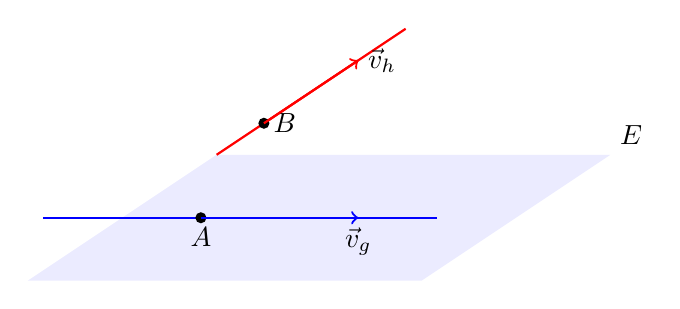
\begin{tikzpicture}[
    x={(1cm,0cm)},
    y={(0.6cm,0.4cm)},
    z={(0cm,1cm)}
]

% --- Ebene E: z = 0 ---
\fill[blue!20,opacity=0.4]
(0,0,0) -- (5,0,0) -- (5,4,0) -- (0,4,0) -- cycle;

\node at (5,4,0) [above right] {$E$};

% --- Gerade g in der Ebene ---
\coordinate (A) at (1,2,0);
\draw[thick,blue] ($(A)+(-2,0,0)$) -- ($(A)+(3,0,0)$);
\fill (A) circle (2pt);
\node[below] at (A) {$A$};

% Richtungsvektor g
\draw[->,thick,blue] (A) -- ++(2,0,0);
\node[below] at ($(A)+(2,0,0)$) {$\vec v_g$};

% --- Gerade h parallel zur Ebene ---
\coordinate (B) at (3,0,2);
\draw[thick,red] ($(B)+(0,-1,0)$) -- ($(B)+(0,3,0)$);
\fill (B) circle (2pt);
\node[right] at (B) {$B$};

% Richtungsvektor h
\draw[->,thick,red] (B) -- ++(0,2,0);
\node[right] at ($(B)+(0,2,0)$) {$\vec v_h$};

\end{tikzpicture}
\end{center}
\index{Abstand!Gerade zu windschiefer Geraden}
\end{theorem}

\begin{example}
Seien $g:\vv{x}=\colvec[3]{1}{4}+\lambda \colvec[2]{0}{1}$ und $h:\vv{x}=\colvec[4]{2}{1}+\mu \colvec[4]{-2}{0}$ Geradengleichungen. Ganz konkret erhalten wir eine Ebene nun, indem wir die Richtungsvektoren als Richtungsvektoren der Ebene interpretieren und den Aufpunkt von $g$ angeben. Denn so stellen wir sicher, dass $g$ in $E$ verläuft und $h$ echt parallel zu $E$ liegt (siehe Satz \ref{Satz:LageEbeneGerade}). Für die Ebene $E$ erhalten wir
\[ E: \vv{x} = \colvec[3]{1}{4} + \lambda \colvec[2]{0}{1} + \mu \colvec[4]{-2}{0}   \]
Das restliche Vorgehen ist wieder dem Vorgehen aus Beispiel \ref{Bsp:Distance_PunktEbene} gleich.
\end{example}

\begin{theorem} \textbf{(Schnittwinkel mit Ebenen und Geraden)} \index{Schnittwinkel mit Ebenen und Geraden} \par
\begin{enumerate}
\item Seien $g$ und $h$ Geraden mit Richtungsvektoren $\vv{u}$ und $\vv{v}$. Dann gilt für den Schnittwinkel der Geraden
\[ \cos \varphi = \dfrac{|\vv{u} \circ \vv{v}|}{|\vv{u}| \cdot |\vv{v}|}\]
\item Seien $E$ und $F$ Ebenen mit Normalenvektoren $\vv{n}$ und $\vv{m}$. Dann gilt für den Schnittwinkel der Ebenen
\[ \cos \varphi = \dfrac{|\vv{n} \circ \vv{m}|}{|\vv{n}| \cdot |\vv{m}|}\]
\item Sei $E$ eine Ebene mit Normalenvektor $\vv{n}$ und $g$ eine Gerade  mit Richtungsvektor $\vv{u}$. Dann gilt für den Schnittwinkel $\varphi$ der Ebene mit der Geraden
\[ \sin \varphi = \dfrac{|\vv{u} \circ \vv{n}|}{|\vv{u}| \cdot |\vv{n}|}\]
Für den Winkel $\beta = \ang{90}-\varphi$ gilt dagegen
\[ \cos \beta = \dfrac{|\vv{u} \circ \vv{n}|}{|\vv{u}| \cdot |\vv{n}|}\]
\end{enumerate}
\label{Satz:SchnittwinkelEbeneGerade}
\end{theorem}

\begin{example}
Gegeben ist die Gerade $g:\vv{x}=\colvec[2]{1}{0}+\lambda \colvec[-2]{1}{2}$ mit der Ebene $E:\vv{x}=\colvec[2]{1}{0}+\lambda \colvec[-1]{2}{2}+\mu \colvec[-2]{1}{0}$. Um den Schnittwinkel zu berechnen, ermitteln wir zuerst den Normalenvektor mittels des Kreuzproduktes:
\[ \vv{n}  = \colvec[-1]{2}{2} \times \colvec[-2]{1}{0} = \colvec[-2]{-4}{3}  \]
Das Skalarprodukt mit dem Richtungsvektor von $g$ ergibt 
\[ \vv{u} \circ \vv{n} = (-2) \cdot (-2) + 1 \cdot (-4) + 2 \cdot 3 = 6 \]
und $|\vv{u}| = 3$ sowie $|\vv{n}|=\sqrt{29}$. Den Winkel erhalten wir nun durch einsetzen in die Formel aus \ref{Satz:SchnittwinkelEbeneGerade}:
\[ \varphi = \sin^{-1} \mleft( \dfrac{\vv{u}\circ \vv{n}}{|\vv{u}| \cdot |\vv{n}|}  \mright) = \sin^{-1}\mleft( \dfrac{6}{3 \cdot \sqrt{29}}  \mright) \approx \ang{21,80} \]
\end{example}

\subsection{Kugeln im Raum}
In diesem Kapitel wollen wir uns mit Kugeln im Raum beschäftigen. Bevor wir dies allerdings tun, gehen wir einen Schritt zurück und überlegen uns, wie wie einen Kreis im $\R^2$ beschreiben können: \par
Ein Punkt $X(x_1|x_2)$ liegt genau dann auf einem Kreis mit Mittelpunkt $M$ und Radius $r$, wenn gilt:
\[ |\vv{MX}| = r \Leftrightarrow (x_1-m_1)^2+(x_2-m_2)^2 = r^2  \]

Wir erkennen hier bereits, dass wir mit der Erweiterung der dritten Dimension eine Kugel vektoriell beschreiben können. Das führt uns zum folgenden Satz:

\begin{definition}
Eine \textbf{Kugel} mit Radius $r$ und Mittelpunkt $M(m_1|m_2|m_3)$ ist die Menge aller Punkte $X(x_1|x_2|x_3)$, für die gilt: \index{Kugel!Beschreibung im $\R^3$}
\[  (x_1-m_1)^2+(x_2-m_2)^2 + (x_3-m_3)^2 = r^2  \]
\end{definition}

Nun stellt sich die Frage, ob ein gegebener Punkt innerhalb, außerhalb oder auf der Kugel befindet. 

\begin{theorem} \textbf{(Lagebeziehungen zwischen Kugel und Punkt)} \par
Sei $X$ ein Punkt und sei eine Kugel mit Radius $r$ und Mittelpunkt $M$ gegeben. Dann gilt:
\begin{enumerate}
\item $(x_1-m_1)^2+(x_2-m_2)^2 + (x_3-m_3)^2 = r^2 \Rightarrow$ Der Punkt liegt auf der Kugel.
\item $(x_1-m_1)^2+(x_2-m_2)^2 + (x_3-m_3)^2 < r^2 \Rightarrow$ Der Punkt ist im Inneren der Kugel.
\item $(x_1-m_1)^2+(x_2-m_2)^2 + (x_3-m_3)^2 > r^2 \Rightarrow$ Der Punkt befindet sich außerhalb der Kugel.
\end{enumerate}
\index{Kugel!Lagebeziehung mit Punkt}
\end{theorem}

\begin{example}
Sei eine Kugel mit Mittelpunkt $M(1|1|1)$ und Radius $r=3$ gegeben. Dann liegt der Koordinatenursprung $(0|0|0)$ in der Kugel, denn $(x_1-m_1)^2+(x_2-m_2)^2 + (x_3-m_3)^2 = 1^2+1^2+1^2 =  3 < 3^2 = 9$. Betrachten wir den Punkt $P(4|-2|4)$, so stellen wir durch Einsetzen in die Gleichung der Kugel fest:
\[  (x_1-m_1)^2+(x_2-m_2)^2 + (x_3-m_3)^2 = (-3)^2 + (3)^2 + (-3)^2 = 27 > 9 = r^2  \]
Also liegt $P$ außerhalb der Kugel. 
\end{example}

Unterbewusst haben wir bereits den Abstand des Punktes mit der Kugel bestimmt. Dieses Prinzip können wir auch für Geraden und später Ebenen erweitern. 


\begin{theorem} \textbf{(Lagebeziehungen zwischen Kugel und Gerade)} \par
Sei $g$ eine Gerade und sei eine Kugel mit Radius $r$ und Mittelpunkt $M$ gegeben. Dann gilt mit dem Abstand $d$ zwischen $M$ und der Geraden:
\begin{enumerate}
\item $d=r \Rightarrow$ Die Gerade berührt die Kugel in genau einem Punkt. $g$ heißt in diesem Fall Tangente.
\item $d<r\Rightarrow$ Die Gerade schneidet die Kugel in genau zwei Punkten. 
\item $d>r \Rightarrow$ Gerade und Kugel schneiden sich nicht.
\end{enumerate}
\index{Kugel!Lagebeziehung mit Gerade}
\end{theorem}

\begin{example}
Betrachten wir die Kugel mit Radius $r=9$ und Mittelpunkt $(0|0|0)$. Zur Untersuchung ziehen wir die Gerade $g:\vv{x}=\colvec[3]{3}{0}+\lambda	\colvec[1]{1}{1}$ hinzu. Dazu bestimmen wir erst den Abstand:
\[ \colvec[3+\lambda]{3+\lambda}{\lambda} \circ \colvec[1]{1}{1} \stackrel{!}{=} 0 \Rightarrow \lambda = -2  \]
Damit erhalten wir den Lotfußpunkt $F(1|1|-2)$ und damit den Abstand $d=\sqrt{6}$. Dieser Abstand ist offenbar kleiner als $9$, wodurch wir die Schnittpunkte mit der Kugel bestimmen können. Hierfür setzen wir für in die Kugelgleichung einen allgemeinen Geradenpunkt ein und lösen nach $\lambda$ auf:
\[ (g_1-m_1)^2+(g_2-m_2)^2 + (g_3-m_3)^2 = (3+\lambda)^2 + (3+\lambda)^2 + (0+\lambda)^2 = r^2 = 81\]
Auflösen nach $\lambda$:
\[  (3+\lambda)^2 + (3+\lambda)^2 + (0+\lambda)^2 - 81 = 0 \]
\[ \lambda^2 + 4\lambda - 63 = 0 \Rightarrow \lambda_{1/2} = -2 \pm 5 \]
Durch einsetzen der zwei Werte erhalten wir $P(6|6|3)$ und $Q(-4|-4|-7)$ als Schnittpunkte der Geraden mit der Kugel.
\end{example}

\begin{theorem} \textbf{(Lagebeziehungen zwischen Kugel und Ebene)} \par
Sei $E$ eine Ebene und sei eine Kugel mit Radius $r$ und Mittelpunkt $M$ gegeben. Dann gilt mit dem Abstand $d$ zwischen $M$ und der Ebene:
\begin{enumerate}
\item $d=r \Rightarrow$ Die Ebene berührt die Kugel in genau einem Punkt $P$. Dabei bildet $\vv{MP}$ einen Normalenvektor dieser Tangentialebene.
\item $d<r\Rightarrow$ Die Ebene schneidet die Kugel in einem Kreis. 
\item $d>r \Rightarrow$ Ebene und Kugel schneiden sich nicht.
\end{enumerate}
\index{Kugel!Lagebeziehung mit Ebene}
\end{theorem}

\begin{example}
Gegeben ist die Kugel mit Kugelgleichung $x^2+y^2+z^2=4$ und die Ebene $E:z-2=0$. Für die Kugel erkennen wir den Mittelpunkt im Koordinatenursprung, und für den Radius lesen wir $r=\sqrt{4}=2$ ab. Durch Anwenden des Satzes \ref{Satz:Distance_PunktEbene} erhalten wir $d=2$. Da der Radius dem Abstand entspricht, ist $E$ eine Tangentialebene.
\begin{center}
\begin{tikzpicture}[tdplot_main_coords, scale=1.5]

% Achsen
\draw[->] (-3,0,0) -- (3,0,0) node[anchor=north east]{$x$};
\draw[->] (0,-3,0) -- (0,3,0) node[anchor=north west]{$y$};
\draw[->] (0,0,-1) -- (0,0,3) node[anchor=south]{$z$};

% Kugel (Drahtgitter)
\foreach \phi in {0,20,...,180} {
    \draw[red]
        plot[domain=0:360, samples=50]
        ({2*sin(\phi)*cos(\x)},
         {2*sin(\phi)*sin(\x)},
         {2*cos(\phi)});
}

\foreach \theta in {0,30,...,330} {
    \draw[red]
        plot[domain=0:180, samples=50]
        ({2*sin(\x)*cos(\theta)},
         {2*sin(\x)*sin(\theta)},
         {2*cos(\x)});
}

% Tangentialebene z = 2
\filldraw[blue!40, opacity=0.5]
    (-2,-3,2) -- (4,-3,2) -- (4,3,2) -- (-2,3,2) -- cycle;

% Berührpunkt
\filldraw[black, thick] (0,0,2) circle (0.05);
\node[right] at (0,0,2) {$P(0,0,2)$};

\draw[->, blue, thick] (0,0,2) -- (0,0,1) node[anchor=north west]{$\vv{n}$};

\end{tikzpicture}
\end{center}
Verschieben wir die gleiche Ebene ein Stück nach unten, so schneidet die Ebene die Kugel in einem Kreis. Wählen wir beispielsweise $E':z-1=0$, so können wir den Radius des Kreises, der den Schnitt aus Kugel und Ebene markiert, mit dem Satz des Pythagoras berechnen. Die folgende Skizze veranschaulicht das Vorgehen:
\begin{center}
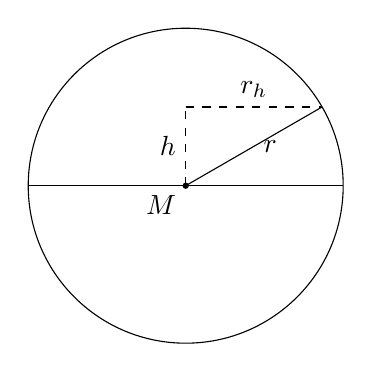
\begin{tikzpicture}[scale=1]

% Radius
\def\r{2}
\def\h{1}

% Kreis
\draw (0,0) circle (\r);

% Mittelpunkt
\fill (0,0) circle (0.04);
\node[below left] at (0,0) {$M$};

% Waagrechter Durchmesser
\draw (-\r,0) -- (\r,0);

% Höhe h
\draw[dashed] (0,0) -- (0,\h);
\node[left] at (0,\h/2) {$h$};

% Punkt auf dem Kreis
\coordinate (P) at ({sqrt(\r*\r-\h*\h)},\h);

% r_h
\draw[dashed] (0,\h) -- (P);
\node[above] at ({sqrt(\r*\r-\h*\h)/2},\h) {$r_h$};

% Radius r
\draw (0,0) -- (P);
\node[right] at ({sqrt(\r*\r-\h*\h)/2},{\h/2}) {$r$};
\end{tikzpicture}
\end{center}
Für den Radius der Kugel $r_h$ gilt: $r^2 = h^2 + r_h^2$. Da $r=2$ gilt, und mit der Gleichung $h=z_{\mathrm{Ebene}}-z_{\mathrm{Mittelpunkt}} = 1 - 0 = 1$ ist, folgt
\[ r_h = \sqrt{r^2-h^2} = \sqrt{4-1} = \sqrt{3}   \] 
Der Radius des Kreies, der beim Schnitt der Ebene $E'$ und der Kugel entsteht, beträgt also $r_h=\sqrt{3}$. \par
\textit{Hinweis:} Im Allgemeinen gilt $h=d(E,M)$, also ist $h$ der Abstand zwischen Mittelpunkt im Kreis und der Ebene. Da $E'$ parallel zur x-y-Ebene liegt, wurde die Rechnung vereinfacht.
\end{example}

\newpage
\section{Stochastik, Statistik und Kombinatorik}
In diesem Kapitel wollen wir uns mit drei mathematischen Teilgebieten beschäftigen. Die Kombinatorik beschäftigt sich mit dem geschickten Zählen von mathematischen Objekten beschäftigt. In der Sochastik geht es um die Wahrscheinlichkeitsrechnung, im speziellen von Zufallsexperimenten. Die Statistik wiederum untersucht Daten. Wir wollen uns zuerst mit Grundbegriffen der Stochastik außeinandersetzen, dann einen Exkurs in die Kombinatorik wagen, um anschließend stochastische Zusammenhänge gut berechnen zu können. Anschließend betrachten wir in der Statistik die wesentlichen Lehrplaninhalte, bevor wir im letzten Teilkapitel die analytische Stochastik mittels der Gauß'schen Glockenkurve untersuchen.

\subsection{Grundlagen der Stochastik}
Bei der Untersuchung von Zufallsexperimenten treten einige Begriffe immer wieder auf. Deshalb wollen wir gleich am Anfang des Kapitels wichtige Begriffe nennen.

\begin{definition} \textbf{(Zufallsexperimente)} \par
\begin{enumerate}
\item Ein Zufallsexperiment\index{Zufallsexperiment} ist ein Vorgang mit ungewissem Ausgang, der beliebig oft unter den gleichen Bedingungen wiederholbar ist und bei dem mehrere Ergebnisse möglich sind.
\item Ein Ergebnis\index{Ergebnis} ist ein einzelner möglicher Ausgang eines Zufallsexperiment. Man bezeichnet ihn mit $\omega$. Die Menge aller Ergebnisse bezeichnet man mit $\Omega$.
\item Ein Ereignis\index{Ereignis} ist eine Teilmenge der Ergebnismenge.
\item Für ein Ereignis $A$ heißt $\overline{A}=\Omega \setminus A$ Gegenereignis\index{Gegenereignis}. Es besteht aus allen Ergebnissen, die nicht in $A$ enthalten sind.
\end{enumerate}
\label{Def:Zufallsexperiment}
\end{definition}

\begin{example}
Das Werfen einer Münze ist ein Zufallsexperiment. Es kann beliebig oft unter den gleichen Bedingungen wiederholt werden, und die Ergebnisse Kopf und Zahl sind vorher ungwiss. Die Ergebnismenge eines (fairen) Münzwurfs besteht also aus $\Omega=\{k,z\}$, wobei $k$ für \glqq Kopf\grqq \ und $z$ für \glqq Zahl\grqq \ steht. \par
Betrachten wir nun einen fairen Würfel, der geworfen wird. Die Ergebnismenge lautet hierfür $\Omega=\{1,2,3,4,5,6\}$. Sei $A$: \glqq Es wird eine Sechs gewürfelt.\grqq \ nun ein Ereignis. Es gilt $A=\{6\}$. Ein Gegenereignis hierzu könnte lauten: \glqq Es wird keine Sechs gewürfelt.\grqq  \ Allemal gilt
\[ \overline{A} = \Omega \setminus A = \{1,2,3,4,5,6\} \setminus \{6\} = \{1,2,3,4,5\}  \]
Alle Ergebnisse außer die Ergebnisse aus $A$ sind Teil des Gegenereignisses $\overline{A}$. 
\end{example}

Ein wichtiges Gesetz der Stochastik ist das Gesetz der großen Zahlen. Es besagt, dass die relative Häufigkeit eines Zufallsergebnisses dem theoretischen Wert näher kommt, wenn man das Zufallsexperiment oft genug wiederholt. Man kann es mit einem Grenzwert aus der Analysis vergleichen.

\begin{definition} Ein Zufallsexperiment heißt \textbf{Laplace-Experiment}, wenn alle Ergebnisse die gleiche Wahrscheinlichkeit besitzen. 
\end{definition}

\begin{example}
Wir wollen uns ein Laplace-Experiment anhand eines Baumdiagramms vorstellen. Dafür betrachten wir die Augenzahl eines Würfels. Jede Seite ist gleich wahrscheinlich, und beim zwei-maligen Würfeln erhalten wir folgendes angedeutete Baumdiagramm:



% Set the overall layout of the tree
\tikzstyle{level 1}=[level distance=5.5cm, sibling distance=3.5cm]
\tikzstyle{level 2}=[level distance=6.5cm, sibling distance=2cm]

% Define styles for bags and leafs
\tikzstyle{bag} = [text width=4cm, text centered,  inner sep=1pt]
\tikzstyle{end} = [circle, minimum width=3pt,fill, inner sep=0pt]

\begin{center}
\begin{tikzpicture}[grow=right, sloped, scale=0.8]
\tikzset{frontier/.style={distance from root=150pt}}

\node {}
    child {
      node[bag] {6}        
        child {
            node[end, label=right:
                {$(6,6)$}] {}
            edge from parent
            node[above] {}
            node[below]  {$\frac{1}{6}$}
        }
        child {
            node[end, label=right:
                {\ldots}] {}
            edge from parent
            node[above] {}
            node[below]  {\ldots}
        }
        child {
            node[end, label=right:
                {$(6,1)$}] {}
            edge from parent
            node[above] {}
            node[below]  {$\frac{1}{6}$}
        }
        edge from parent 
        node[above] {}
        node[below]  {$\frac{1}{6}$}
}
child {
      node[bag] {\ldots}        
        edge from parent 
        node[above] {}
        node[below]  {}
}
child {
      node[bag] {\ldots}        
        edge from parent 
        node[above] {}
        node[below]  {}
}
child {
      node[bag] {1}        
        child {
            node[end, label=right:
                {$(1,6)$}] {}
            edge from parent
            node[above] {}
            node[below]  {$\frac{1}{6}$}
        }
        child {
            node[end, label=right:
                {$(1,5)$}] {}
            edge from parent
            node[above] {}
            node[below]  {$\frac{1}{6}$}
        }
        child {
            node[end, label=right:
                {$(1,4)$}] {}
            edge from parent
            node[above] {}
            node[below]  {$\frac{1}{6}$}
        }
        child {
            node[end, label=right:
                {$(1,3)$}] {}
            edge from parent
            node[above] {}
            node[below]  {$\frac{1}{6}$}
        }
        child {
            node[end, label=right:
                {$(1,2)$}] {}
            edge from parent
            node[above] {}
            node[below]  {$\frac{1}{6}$}
        }
        child {
            node[end, label=right:
                {$(1,1)$}] {}
            edge from parent
            node[above] {}
            node[below]  {$\frac{1}{6}$}
        }
        edge from parent 
        node[above] {}
        node[below]  {$\frac{1}{6}$}
};

\end{tikzpicture}
\end{center}
Die Ergebnismenge lautet nun $\Omega = \{(1,1), (1,2), \ldots, (6,4), (6,5), (6,6) \}$. Da jede Zahl auf dem Würfel die gleiche Wahrscheinlichkeit hat, nennen wir dieses Zufallsexperiment Laplace-Experiment. \par
Betrachten wir beim einmaligen Werfen das Ereignis $A$: \glqq Die Augensumme ist durch drei teilbar.\grqq \ Dann sehen wir, dass die Ergebnismenge $A=\{3,6 \}$ ist, denn alle anderen Zahlen sind nicht durch $3$ teilbar. Das Gegenereignis $\overline{A}$ lautet: \glqq Die Augensumme ist nicht durch drei teilbar.\grqq \ Die Ergebnismenge dazu lautet $\overline{A}=\{ 1,2,4,5 \}$. Die Wahrscheinlichkeit bei Laplace-Experimenten ermitteln wir wiefolgt:
\[ P(A)=\dfrac{\text{Anzahl der günstigen Ereignisse}}{\text{Anzahl der möglichen Ereignisse}} = \dfrac{2}{6} = \dfrac{1}{3} \approx \SI{33,33}{\percent} \]
\label{Bsp:ZweimalWürfeln}
\end{example}

Anhand des obigen Beispiels kann man auch die Formel zur Berechnung eines Laplace-Experiments erkennen. Wir fassen diese Erkenntnis nochmals im nächsten Satz zusammen, wobei man sich am Beispiel von oben orientieren kann.

\begin{theorem}
Bei einem Laplace-Experiment ermittelt man die Wahrscheinlichkeit durch die Formel
\[ P(A)=\dfrac{\text{Anzahl der günstigen Ereignisse}}{\text{Anzahl der möglichen Ereignisse}} \]
\end{theorem}

Nun wollen wir uns die Verknüpfung von Ereignissen ansehen. Dafür ziehen wir auch Mengendiagramme und Vierfeldertafeln hinzu. Eine Verknüpfung kann mathematisch mit drei Mengenoperatoren dargestellt werden.

\begin{definition} \index{Mengenoperatoren} \
\begin{enumerate}
\item Die Schnittmenge\index{Schnittmenge} $A \cap B$ ist die Menge aller Elemente, die in $A$ \textbf{und} $B$ sind.
\item Die Vereinigungsmenge\index{Vereinigungsmenge} $A\cup B$ ist die Menge aller Elemente, die in $A$ \textbf{oder} in $B$ sind.
\item Die Mengendifferenz\index{Mengendifferenz} $A \setminus B$ ist die Menge aller Elemente $a\in A$, die nicht in $B$ enthalten sind.
\end{enumerate}
\end{definition}

\begin{example}
Betrachten wir die Mengen $M=\{ 0, 1\}$ und $N=\{ 1, 2, 3\}$. Dann gilt:
\begin{enumerate}
\item $M \cap N = \{ 1\}$
\item $M \cup N = \{ 0, 1, 2, 3\}$
\item $M \setminus N =  \{ 0\}$ und $N \setminus M = \{ 2,3\}$
\end{enumerate}
\end{example}

Diesen Sachverhalt kann man in Mengendiagrammen (Venn-Diagrammen) ausdrücken.

\begin{definition}
Verknüpfte Zufallsexperimente, wo zwei oder mehr Ereignisse beschrieben und untersucht werden. Sind $A$ und $B$ die betrachteten Ereignisse, so können sie in einem Venn-Diagramm dargestellt werden. 

\begin{center}
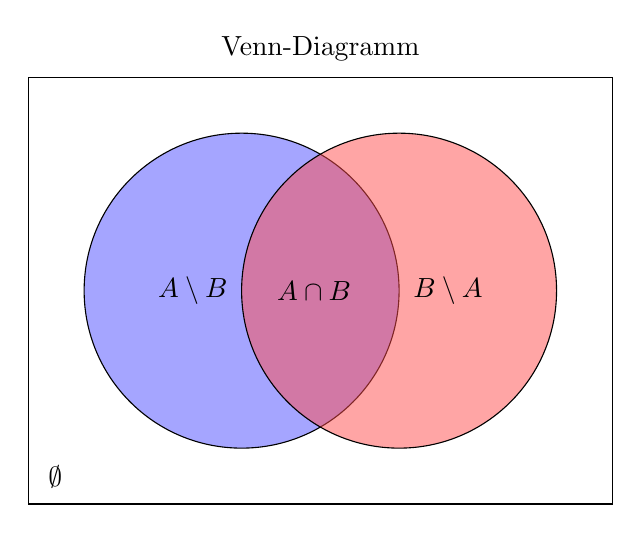
\begin{tikzpicture}
\def\radius{2cm}
\def\mycolorbox#1{\textcolor{#1}{\rule{2ex}{2ex}}}
\colorlet{colori}{blue!70}
\colorlet{colorii}{red!70}

\coordinate (ceni);
\coordinate[xshift=\radius] (cenii);

\draw[fill=colori,fill opacity=0.5] (ceni) circle (\radius);
\draw[fill=colorii,fill opacity=0.5] (cenii) circle (\radius);

\draw  ([xshift=-20pt,yshift=20pt]current bounding box.north west) 
  rectangle ([xshift=20pt,yshift=-20pt]current bounding box.south east);

\node[yshift=10pt] at (current bounding box.north) {Venn-Diagramm};


\node[xshift=-.6\radius] at (ceni) {$A\setminus B$};
\node[xshift=.6\radius] at (cenii) {$B \setminus A$};
\node[xshift=.9\radius] at (ceni) {$A\cap B$};
\node[xshift=10pt,yshift=10pt] at (current bounding box.south west) {$\emptyset$};
\end{tikzpicture}
\end{center}
\index{Venn-Diagramm} \index{Verknüpfte Zufallsexperimente \index{Mengendiagramm}}
\end{definition}

Anhand dieses Schaubildes kann man sich überlegen, wie sich die Wahrscheinlichkeit $P(A\cup B)$ berechnet. $A$ repräsentiert den blauen Kreis, und $B$ den roten Kreis. Würden wir sagen $P(A\cup B)=P(A)+P(B)$, so würden wir die Schnittmenge doppelt zählen, denn jedes Ereignis der Schnittmenge wäre dann durch $P(A)$ und $P(B)$ doppelt repräsentiert. Deshalb subtrahieren wir einmal die Schnittmenge und kommen um folgenden Satz:

\begin{theorem}
Für ein verknüpftes Zufallsexperiment mit Ereignissen $A$ und $B$ gilt:
\[ P(A\cup B) = P(A) + P(B) - P(A\cap B)\]
\index{Formel!für verknüpfte Zufallsexperimente}
\label{Satz:VerknüpftesZufallsexperiment}
\end{theorem}

\begin{example}
Gegeben ist die Vierfeldertafel \index{Vierfeldertafel}
\begin{center}
\begin{tabular}{c | c | c | c}
 & $A$ & $\overline{A}$ & \\
 \hline
 $B$ & $\num{0,21}$ & $\num{0,02}$ & $\num{0,23}$ \\
 \hline
 $\overline{B}$ & $\num{0,25}$ & $\num{0,52}$ & $\num{0,77}$ \\
 \hline
 & $\num{0,46}$ & $\num{0,54}$ & $\num{1}$
\end{tabular}
\end{center}
Für $P(A\cup B)$ gilt in diesem Beispiel $P(A\cup B)=\num{0,46}+\num{0,23}-\num{0,21}=\num{0,48}$. 
\end{example}

Als letztes wollen wir uns in diesem Unterkapitel noch den Pfadregeln beim Baumdiagramm widmen.

\begin{theorem} \textbf{(Pfadregeln)} \
\begin{enumerate}
\item Die Wahrscheinlichkeiten entlang eines Pfades werden stets multipliziert.
\item Die Wahrscheinlichkeiten verschiedener Ergebnisse werden addiert, wenn sie zum gleichen Ereignis gehören.
\end{enumerate}
\index{Pfadregeln}
\end{theorem}

\begin{example}
Betrachten wir erneut die Situation aus Beispiel \ref{Bsp:ZweimalWürfeln} und das dazugehörige Baumdiagramm. Sei $B$: \glqq Die Summe der Augenwürfel ist gleich vier\grqq \ unser Ereignis. Dann können wir die einzelnen Pfade bestimmen. Es gilt $B=\{ (1,3), (3,1), (2,2)  \}$. Die Wahrscheinlichkeit eines solchen Pfades ist $P((1,3))=P((3,1))=P((2,2))=\dfrac{1}{6}\cdot \dfrac{1}{6} = \dfrac{1}{36}$. Hierbei haben wir die erste Pfadregel verwendet. Die zweite Pfadregel sagt nun aus, dass wir die Wahrscheinlichkeiten dieser Ergebnisse addieren dürfen, um die Wahrscheinlichkeit des Ereignisses zu erhalten: $P(B)=\dfrac{1}{36}+\dfrac{1}{36}+\dfrac{1}{36}=\dfrac{3}{36}=\dfrac{1}{12} \approx \SI{8,33}{\percent}$
\end{example}

\begin{definition}
Sind $A$ und $B$ beliebige Ereignisse und $P(A)>0$ ist, dann heißt
\[ P_A(B)= \dfrac{P(A \cap B)}{P(A)}\]
die \textbf{bedingte Wahrscheinlichkeit} von $A$ vorausgesetzt $B$ oder auch \textbf{Wahrscheinlichkeit von $\mathbf{A}$ unter der Bedingung $\mathbf{B}$}.
\end{definition}

\begin{theorem}
Sind $A$ und $B$ beliebige Ereignisse. Dann sind folgende Aussagen äquivalent:
\begin{enumerate}
\item $A$ und $B$ sind stochastisch unabhängig.
\item $P_B(A)=P(A)$
\item $P_A(B)=P(B)$
\item $P(A) \cdot P(B) = P(A\cap B)$
\end{enumerate}
\end{theorem}

\begin{example}
Gegeben sei ein fairer Standardwürfel. Weiterhin bezeichnet $A=\{1,2,3\}$ das Ereignis $A$, dass bei einem Wurf eine Eins, Zwei oder Drei gewürfelt wurde.
\begin{enumerate}
\item Sei $B=\{4,5\}$. Dann ist $A\cap B = \{ \}$ die leere Menge. $A$ und $B$ haben also keine gemeinsamen Elemente. Es gilt deshalb
\[ P_A(B) = \dfrac{P(A\cap B)}{P(A)} = \dfrac{0}{P(A)} = P_B(A) = \dfrac{P(A\cap B)}{P(B)} = \dfrac{0}{P(B)} = 0 \]
Da sowohl $P(A)$ als auch $P(B)$ eine Wahrscheinlichkeit besitzen, die größer als $0$ ist, sind die Ereignisse stochastisch abhängig. (\textit{Wenn ich weiß, dass eine Eins, Zwei oder Drei gewürfelt wurde, kann ich ausschlißen, dass eine Vier oder Fünf gewürfelt wurde.})
\item Ist $B$ das Ereignis, dass eine gerade Zahl gewürfelt wurde, so ist $B=\{2,4,6\}$. Prüfe, ob $A$ und $B$ stochastisch unabhängig sind:
\[ P(B)=\dfrac{1}{2} \quad P_A(B) = \dfrac{P(A\cap B)}{P(A)} = \dfrac{P(\{ 2\}) }{\num{0,5}} = \dfrac{1}{3} \neq \dfrac{1}{2}\]
Also sind $B$ und $A$ stochastisch abhängig!
\item Weiterhin wird der zweimalige Wurf des Würfels betrachtet. Die Ergebnisse $C$: \glqq Es wird im ersten Wurf eine Primzahl gewürfelt\grqq \ und $D$: \glqq Im zweiten Wurf ist die Augensumme ungerade\grqq \ sind stochastisch unabhängig. Denn für $C$ gilt $P(C)=\frac{1}{2}$, denn die Zahlen $2$,$3$ und $5$ sind Primzahlen. Für $D$ gilt ebenfalls $P(D)=\frac{1}{2}$, da die Zahlen Eins, Drei und Fünf ungerade sind. Da sich die Wahrscheinlichkeit von $D$ durch das Ergebnis des ersten Wurfes nicht beeinflusst, sind die Ereignisse stochastisch unabhängig.
\end{enumerate}
\end{example}

\newpage
\subsection{Kombinatorik}
\label{ssec:Kombinatorik}
\index{Urnenmodell}Die Kombinatorik beschäftigt sich, wie anfangs erwähnt, mit dem geschickten Zählen. Hierzu führen wir den Begriff des Urnenmodells ein, das in der Stochastik oft verwendet wird. Hierzu gehen wir davon aus, dass wir eine Urne mit einer Anzahl an Kugeln haben, aus der wir blind eine Anzahl an Kugeln herausnehmen. 

\begin{theorem} \textbf{(Ziehen mit Zurücklegen und Beachtung der Reihenfolge)} \par
In einem Urnenmodell mit $n$ Kugeln werden $k$ Kugeln mit Zurücklegen gezogen. Die Anzahl möglicher Kombinationen, wenn man die Reihenfolge beachtet, wird durch den Term
\[ \underbrace{n \cdot n \cdot \ldots \cdot n}_{\mathrm{k-Mal}} = n^k \]
beschrieben.
\end{theorem}

Legt man die Kugeln nach dem Ziehen in die Urne nicht mehr zurück, so ändert sich die Anzahl an Möglichkeiten. Während es für den ersten Zug noch $n$ Möglichkeiten gibt, gibt es für den zweiten Zug nur noch $(n-1)$ Möglichkeiten. Diese Erkenntnis führt uns zum Begriff der Fakultät:

\begin{definition}
Für eine natürliche Zahl $n\in \N$ heißt 
\[ n! := n \cdot (n-1) \cdot (n-2) \cdot \ldots \cdot 2 \cdot 1\]
Fakultät. \index{Fakultät}
\end{definition}

\begin{example}
Es gilt $5!=5\cdot 4 \cdot 3 \cdot 2 \cdot 1 = 120$.
\end{example}

Mittels der Fakultät können wir das Ziehen ohne Zurücklegen systematisch gut beschreiben. Zuerst soll die Reihenfolge von Relevanz sein. 

\begin{theorem} \textbf{(Ziehen ohne Zurücklegen mit Beachtung der Reihenfolge)} \par
In einem Urnenmodell mit $n$ Kugeln werden $k\leq n$ Kugeln ohne Zurücklegen gezogen. Die Anzahl möglicher Kombinationen erhält man durch
\[ n\cdot (n-1) \cdot \ldots \cdot (n-k+2) \cdot (n-k+1) = \dfrac{n \cdot \ldots (n-k+1) \cdot (n-k) \cdot (n-k-1) \cdot \ldots \cdot 2 \cdot 1}{(n-k) \cdot (n-k-1) \cdot \ldots \cdot 2 \cdot 1} \] \[ = \dfrac{n!}{(n-k)!}  \]
\end{theorem}

\begin{example}
Acht Läuferinnen und Läufer sprinten in einem Wettkampf gegeneinander. Wir wollen uns überlegen, wie viele mögliche Siegerehrungen es gibt, wenn nur die ersten drei Plätze etwas gewinnen. Die Reihenfolge ist relevant, da der erste Preis höher dotiert ist als der zweite Platz. Außerdem handelt es sich um eine Analogie zum Urnenmodell ohne Zurücklegen, denn der achte Platz kann nicht gleichzeitig sechster Platz sein. Die möglichen Podestplätze ermitteln wir durch
\[ \dfrac{8!}{(8-3)!} = 8 \cdot 7 \cdot 6 = 336\]
Also sind 336 mögliche Kombinationen für die Siegerplätze möglich. Für die Reihenfolge, in der die Läuferinnen und Läufer ins Ziel kommen, gibt es sogar $8!=40320$ Möglichkeiten.
\label{Bsp:Läufer}
\end{example}

Ist die Reihenfolge egal, so ist die Überlegung die Folgende: Beim dreimaligen Ziehen gibt es für jeden Fall genau $3!=3\cdot 2 \cdot 1 = 6$ Möglichkeiten, dass beispielsweise Läufer $A,B,C$ ins Ziel kommen. Da jede Variante davon einzeln im Ziehen mit Reihenfolge ist (Die Kombinationen $(A,B,C), (A,C,B),$ usw. sind verschiedene Möglichkeiten), dividieren wir durch die Anzahl dieser Reihenfolgen. 

\begin{definition} Wir nennen $\colvec{n}{k}=\dfrac{n!}{k! \cdot (n-k)!}$ \textbf{Binomialkoeffizient}. \par
Wörtlich sagt man \glqq n über k\grqq \ oder auch \glqq k von n\grqq.
\index{Binomialkoeffizient}
\end{definition} 

\begin{definition}
Alle möglichen Reihenfolgen von Elementen einer Menge nennt man \textbf{Permutationen}. Für $n$ Elemente gibt es genau $n!$ Permutationen. 
\index{Permutation}
\end{definition}

\begin{example}
Greifen wir nochmals Beispiel \ref{Bsp:Läufer} auf. Da wir $3$ Läuferinnen oder Läufer haben, die auf Siegerplätzen landen, gibt es für drei bestimmte Läuferinnen oder Läufer $\{A,B,C\}$ genau $3!=6$ Möglichkeiten, die Plätze aufzufüllen. Also gibt es $3!$ Permutationen. Explizit sind das die Ergebnisse $(A,B,C), (A,C,B), (B,A,C),$ $(B,C,A), (C,A,B), (C,B,A)$.
\end{example}

\begin{theorem} \textbf{(Ziehen ohne Zurücklegen ohne Beachtung der Reihenfolge)} \par
In einem Urnenmodell mit $n$ Kugeln werden $k\leq n$ Kugeln ohne Zurücklegen gezogen. Die Anzahl möglicher Kombinationen, wenn die Reihenfolge nicht beachtet wird, erhält man durch den Binomialkoeffizienten
\[ \colvec{n}{k}=\dfrac{n!}{k! \cdot (n-k)!}  \]
\end{theorem}

\begin{example}
Für einen Reisenden stellt sich die Frage, welche Bücher er mitnimmt. Im Koffer ist Platz für drei Bücher, in seinem Schrank kann er aus zehn Büchern auswählen. Da hier die Reihenfolge egal ist, wenden wir den Binomialkoeffizienten an. Es gilt also
\[ \colvec{10}{3} = 120\]
\end{example}

\newpage
\subsection{Stochastik der Oberstufe}
\label{ssec:StochDerObst}
Ein zentrales Element der Stochastik ist die Begründung derselben. 1933 versuchte Andrei Kolmogorow, eine theoretische Grundlage für die Wahrscheinlichkeitsrechnung zu liefern. Er publizierte sechs sogenannte \textbf{Axiome}, also Grundaussagen, die festgelegt werden, und deren Richtigkeit hingenommen werden muss. \par
Betrachten wir eine Funktion $P:A\mapsto P(A)$, die einem Ereignis $A$ eine Wahrscheinlichkeit $P(A)$ zuordnen.
\begin{definition} \textbf{(Axiome von Kolmogorow)} \par
Sei $P:A\mapsto P(A)$ eine Funktion, dann heißt $P(A)$ Wahrscheinlichkeitsverteilung, wenn gilt:
\begin{enumerate}
\item $0\leq P(A) \leq 1$,
\item Für die Ergebnismenge $\Omega$ gilt $P(\Omega) = 1$ und
\item falls $A\cap B = \emptyset$, so gilt $P(A \cup B) = P(A)+(B)$.
\end{enumerate}
Hierbei ist $\emptyset$ die leere Menge.
\index{Axiome von Kolmogorow}
\label{Def:Axiome_Kolmogorow}
\end{definition}

Aus diesen drei Grundaxiomen lassen sich unmittelbar Aussagen schließen. Neben Satz \ref{Satz:VerknüpftesZufallsexperiment} sind auch die folgenden zwei Aussagen aus den Axiomen von Kolmogorow ableitbar:

\begin{theorem} \textbf{(Folgerungen der Axiome von Kolmogorow)} \par
Aus den Axiomen von Kolmogorow ergeben sich unmittelbar Folgen. Es gilt:
\begin{enumerate}
\item $P(\overline{A})=1-P(A)$
\item $P(\emptyset)=0$
\end{enumerate}
\end{theorem}
Um zu verstehen, warum die Aussagen aus den Axiomen folgern, folgt hier ein Beweis:

\begin{proof} \
\begin{enumerate}
\item Wir können $P(\overline{A})$ schreiben als $P(\Omega\setminus A)$. Nun gilt weiterhin $(\Omega \setminus A)\cup A=\Omega$. Wörtlich bedeutet das, dass alle Ereignisse darstellbar sind durch alle Ereignisse ohne A, wenn man diese Menge wieder mit A vereinigt. Entfernt man A aus der Menge und fügt es dann wieder hinzu, ändert sich nichts. Ebenfalls gilt $(\Omega \setminus A)\cap A=\emptyset$, denn die Menge $(\Omega \setminus A)$ enthält kein Element aus A, und deshalb haben die beiden Mengen kein Element gemeinsam. Nach Axiom 3 gilt nun $P(\Omega \setminus A) + P(A) = P(\Omega)$, und nach Axiom 2 folgt $P(\Omega \setminus A) + P(A) = 1$. Umgestellt ergibt das nun
\[ 1- P(A) = P(\Omega \setminus A) = P(\overline{A}) \]
\item Es ist $\emptyset \cup \Omega = \Omega$ und $\emptyset \cap \Omega = \emptyset$, also nach Axiom 3: $P(\emptyset)+(P(\Omega) = 1$. Daraus folgt $P(\emptyset)=0$.
\end{enumerate}
\end{proof}

Die Beweise sollen einen Einblick in mathematische Denken geben. Die Sprache der Mathematik ist eine völlig unnatürliche, wenn man sie nicht kennt. Falls du dich also schwer tust, den Beweis der Aussagen nachzuvollziehen, ist das nicht dramatisch! Falls der Beweis dir hilft, zu verstehen, warum die Aussage gilt, ist das gut. Falls er dich verwirrt, so lasse dich davon nicht beirren. 

\begin{example} \ 
\begin{enumerate}
\item Die Funktion $f: x \mapsto x^2$ mit $\Omega=\{2,3\}$ ist keine Wahrscheinlichkeitsverteilung, da $f(2)=4>1$ ist. 
\item Sei $\Omega =\{1,2,3,4,5,6  \}$ und $P(A)=\dfrac{1}{6}$ für alle $A\in \Omega$ für einen Standardwürfelwurf. Dann ist das erste Axiom erfüllt, denn jede Wahrscheinlichkeit für ein Element aus $\Omega$ beträgt $P(A)=\dfrac{1}{6}$. Das zweite Axiom ist auch wahr, denn $P(\Omega) = \dfrac{1}{6}+\dfrac{1}{6}+\dfrac{1}{6}+\dfrac{1}{6}+\dfrac{1}{6}+\dfrac{1}{6}=1$. Auch 3. ist wahr, denn falls $A$ und $B$ zwei Ereignisse sind, die kein gemeinsames Ergebnis haben, so ist nach Satz \ref{Satz:VerknüpftesZufallsexperiment} $P(A\cup B)=P(A)+P(B)-P(A\cap B)$. Da $A\cap B = \emptyset$ ist, ist die Wahrscheinlichkeit $P(A\cap B) = 0$, denn die Wahrscheinlichkeit, keine Eins, Zwei, Drei, Vier, Fünf, oder Sechs zu würfeln, liegt bei Null.
\end{enumerate}
\end{example}

Nun wollen wir uns weiter mit Zufallsgrößen beschäftigen und dabei auf deren Wahrscheinlichkeitsverteilung blicken:

\begin{definition}
Eine Funktion $X$, die jedem Ergebnis $\omega \in \Omega$ eine reelle Zahl $X(\omega)$ zuordnet, heißt \textbf{Zufallsvariable} oder \textbf{Zufallsgröße} auf $\Omega$. Wir schreiben
\[ X:\omega \mapsto X(\omega) \quad \text{mit} \ \omega \in \Omega \ \text{und} \ X(\omega) \in \R  \]
\index{Zufallsgröße}
\end{definition}

Analog dazu können wir auch jedem Wert einer Zufallsgröße eine Wahrscheinlichkeit zuordnen:

\begin{definition}
Für eine Zufallsvariable $X$ ist die \textbf{Wahrscheinlichkeitsfunktion} $W$ jene Funktion, die jedem Wert $x_i \in X$ die Wahrscheinlichkeit $P(X=x_i)$ zuordnet. Wir schreiben
\[ W:x_i \mapsto P(X=x_i)  \]
\index{Funktion!Wahrscheinlichkeits}
\end{definition}

\begin{example}
Bei einem Münzwurf wird $\SI{1}{\euro}$ Einsatz verlangt. Bei Kopf werden $\SI{2}{\euro}$ ausgezahlt, bei Zahl erhält man nichts. Es wird der Gewinn des Zufallsexperiments betrachtet. \par
Die Ergebnismenge lautet $\Omega=\{k,z\}$, wobei $k$ das Ergebnis \glqq Kopf\grqq, $z$ das Ergebnis \glqq Zahl\grqq \ repräsentiert. Nun ist der Gewinn die Zufallsvariable. Für die einzelnen Ergebnisse lauten die Gewinne
\begin{align*}
k \mapsto 1 \\
z \mapsto -1
\end{align*}
Ein häufiger Fehler ist das Verwechseln von Gewinn und Auszahlung: Der Einsatz beträgt schon $\SI{1}{\euro}$ und muss beim Gewinn berücksichtigt werden! Die Wahrscheinlichkeitsfunktion dazu kann geschrieben werden als
\[ W(x_i) = \begin{cases} \num{0,5}, & \text{falls} \ x_i=1 \\ \num{0,5}, & \text{falls} \ x_i=-1  \end{cases}\]
\end{example}

\begin{definition}
Ein Histogramm ist eine grafische Darstellung der Häufigkeitsverteilung. Es erfordert die Einteilung der Daten in Klassen, die eine konstante Breite haben. Der Flächeninhalt eines Rechtecks stellt die Wahrscheinlichkeit dar.
\index{Histogramm}
\end{definition}

\begin{example}
In einer Umfrage wird die Lernzeit von 100 Schülerinnen und Schülern für eine Mathematik-Klausur erfasst. Dabei wurden folgende Ergebnisse notiert:
\begin{center}
\begin{tabular}{c c c}
\toprule
Lernzeitintervall in $\unit{\hour}$ & Anzahl & relative Häufigkeit \\
\midrule
0-2 & 10 & $\num{0,1}$ \\
2-4 & 30 & $\num{0,3}$ \\
4-6 & 40 & $\num{0,4}$ \\
6-8 & 20 & $\num{0,2}$ \\
\bottomrule
\end{tabular}
\end{center}
Da der Intervall jeweils zwei Stunden beträgt, ist die Rechteckbreite von 2 Einheiten in diesem Fall naheliegend. Nun ist die Höhe des Rechtecks zu bestimmen, indem wir die relative Häufigkeit mit der Breite dividieren. Für den Intervall von zwei bis vier Stunden gilt beispielsweise
\[ A_{\mathrm{Säule}}=\num{0,3} = 2 \cdot h \Leftrightarrow h = \dfrac{\num{0,3}}{2} = \num{0,15}\]
\begin{center}
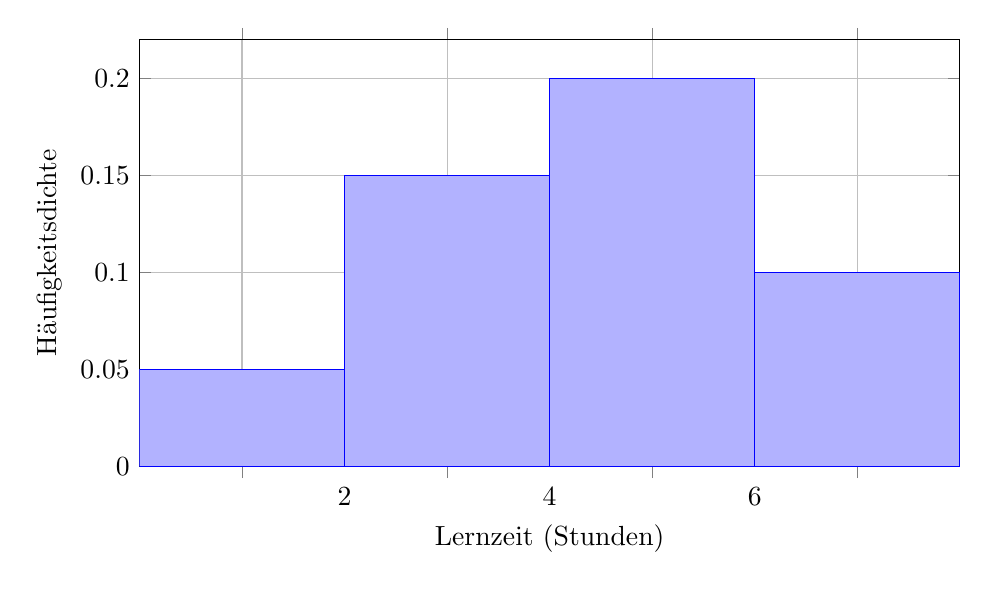
\begin{tikzpicture}
\begin{axis}[
ybar interval,
xmin=0, xmax=8,
ymin=0, ymax=0.22,
xlabel={Lernzeit (Stunden)},
ylabel={Häufigkeitsdichte},
width=12cm,
height=7cm,
grid=both,
scaled y ticks=false,
yticklabel style={/pgf/number format/fixed},
xtick={-1,1,3,5,7,9},
xticklabels={0,2,4,6,8}
]

\addplot coordinates {
(0,0.05)
(2,0.15)
(4,0.20)
(6,0.10)
(8,0)
};

\end{axis}
\end{tikzpicture}

\end{center}
\label{Bsp:Histogramm}
\end{example}

Falls man sich nun die Frage stellt, wie viele Schülerinnen und Schüler höchstens vier Stunden lernen, addiert man die Flächen (relativen Häufigkeiten) der beiden ersten Intervalle. Dieses Überlegung führt uns zur kumulativen Verteilungsfunktion:

\begin{definition}
Die Funktion $F$, die bei einer Zufallsgröße $X$ jeder Zahl $x\in \R$ die Wahrscheinlichkeit $P(X\leq x)$ zuordnet, heißt \textbf{kumulative Verteilungsfunktion}. Wir schreiben
\[ F: x \mapsto P(X\leq x) \quad \text{mit} \ x\in\R, \ P(X\geq x)\in [0,1]\]
\index{Funktion!kumulative Wahrscheinlichkeits}
\end{definition}

\begin{example}
Greifen wir erneut Beispiel \ref{Bsp:Histogramm} auf. Nun betrachten wir aber nichtmehr die einzelnen zweistündigen Intervalle, sondern die kumulative Verteilung. Für einen zufällig ausgewählten Schüler beträgt die Wahrscheinlichkeit, weniger als zwei Stunden zu lernen immer noch $\SI{10}{\percent}$. Für vier oder weniger Stunden addieren wir die Wahrscheinlichkeit der ersten beiden Intervalle: Entweder ist die Person zu zehn Prozent weniger als zwei Stunden mit Lernen beschäftigt, oder sie lernt zwischen zwei und vier Stunden. Das Letztgenannte hat eine Wahrscheinlichkeit von $\SI{30}{\percent}$. Zusammen sind es also $\SI{40}{\percent}$. So führt uns die kumulative Wahrscheinlichkeitsfunktion zu folgendem Graphen:

\begin{center}
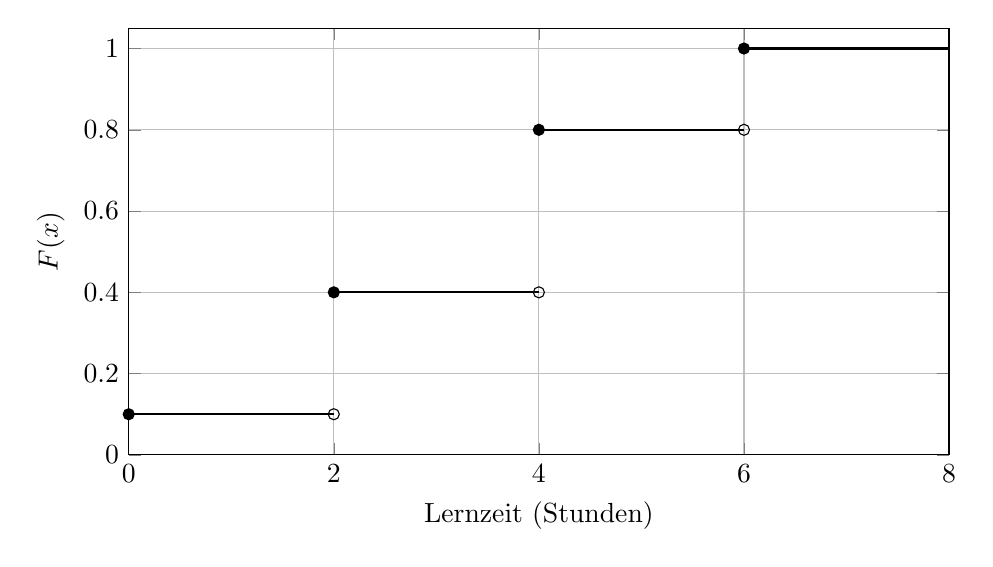
\begin{tikzpicture}
\begin{axis}[
xmin=0, xmax=8,
ymin=0, ymax=1.05,
xlabel={Lernzeit (Stunden)},
ylabel={$F(x)$},
xtick={0,2,4,6,8},
ytick={0,0.2,0.4,0.6,0.8,1},
grid=both,
width=12cm,
height=7cm
]

% horizontale Stücke
\addplot[thick] coordinates {(0,0.1) (2,0.1)};
\addplot[thick] coordinates {(2,0.4) (4,0.4)};
\addplot[thick] coordinates {(4,0.8) (6,0.8)};
\addplot[thick] coordinates {(6,1) (8,1)};

% offene Kreise (linke Seite)
\addplot[only marks, mark=o, mark size=2pt] coordinates {
(2,0.1)
(4,0.4)
(6,0.8)
};

% gefüllte Punkte (rechte Seite)
\addplot[only marks, mark=*, mark size=2pt] coordinates {
(0,0.1)
(2,0.4)
(4,0.8)
(6,1)
};

\end{axis}
\end{tikzpicture}
\end{center}
Um aus dem Graphen die einzelnen Wahrscheinlichkeiten zu ermitteln, ermittelt man die Differenz an der Sprungstelle. So gilt für $x=2$:
\[ \Delta y = \num{0,4}-\num{0,1} = \num{0,3}\]
Die Punkte,die ausgefüllt sind, inkludieren dabei den Wert, also an der Stelle $x=2$ ist der Graph auf Höhe $y=\num{0,4}$. Der offene Kreis hingegegen enthält den Wert selbst nicht. 
\end{example}

Stellen wir uns folgendes Spiel vor: Alice würfelt mit einem sechsseitigen regulären Würfel. Für jede Primzahl erhält Bob zwei Euro, falls keine Primzahl kommt, muss Bob einen Euro in die Kaffeekasse geben. Nun fragt sich Alice zurecht: \glqq Ist das Spiel, was ich da spiele, eigentlich fair?\grqq \par
Um diese Frage zu beantworten, benötigen wir den Begriff des Erwartungswerts.
\begin{definition}
Für eine Zufallsgröße $X$ gilt für den Erwartungswert $E(X)$:
\[ E(X) = \mu = \sum_{i=1}^nx_i \cdot P(X=x_i) = x_1 \cdot P(X=x_1) + x_2 \cdot P(X=x_2) + \ldots + x_n \cdot P(X=x_n) \]
Der Erwartungswert ist eine Art Durchschnittswert bei unendlich vielen Wiederholungen.
\index{Erwartungswert!bei diskreten Zufallsgrößen}
\end{definition}

\begin{example}
Für das oben genannte Spiel zwischen Alice und Bob gibt es zwei Ausgänge, entweder verdient Bob zwei Euro (Primzahl), oder er zahlt einen Euro (keine Primzahl). Die Zahlen (1,4,6) sind keine Primzahlen, also ist die Wahrscheinlichkeit, keine Primzahl zu ziehen: $P(X=-1)=\dfrac{3}{6}=\dfrac{1}{2}$. Die Wahrscheinlichkeit beschreibt bei der Zufallsgröße $X$, die den Gewinn von Bob beschreibt, die Male, wenn Bob einen Euro zahlen muss, also wenn $X=-1$ gilt. Wenn andersherum eine Primzahl gewürfelt wird ($p=\dfrac{1}{2}$), erhält Bob zwei Euro, also ist $X=2$. Wir müssen einen Einsatz hier nicht berücksichtigen, denn das Mitspielen ist kostenlos. Für die zwei Ereignisse bestimmen wir den Erwartungswert nun wiefolgt:
\[ E(X)=  \sum_{i=1}^2 x_i \cdot P(X=x_i) = (-1) \cdot \dfrac{1}{2} + 2 \cdot \dfrac{1}{2} = \num{0,5} \]
Hierbei ist $x_1=-1$ das erste Ereignis (\glqq keine Primzahl\grqq) und $x_2=2$ das zweite Ereignis (\glqq Primzahl\grqq).
\end{example}

Ist das Spiel nun fair? Mathematikerinnen und Mathematiker haben dafür folgendes definiert:

\begin{definition}
Ein Spiel heißt \textbf{fair}, wenn der Erwartungswert des Gewinns für jede Spielerin und jeden Spieler 0 ist.
\index{faires Spiel}
\end{definition}

\begin{example}
Wir stellen fest, dass das Spiel zwischen Alice und Bob nicht fair ist, denn Bobs Gewinn ist im Mittel größer als 0. Wir fragen uns deshalb, wie wir das Spiel fair gestalten können. Es muss also für Bobs Gewinn gelten:
\[ E(X) = x_1 \cdot \dfrac{1}{2} + x_2 \cdot \dfrac{1}{2} \stackrel{!}{=} 0\]
Hierbei ist $x_1$ der Gewinn beim Ereignis \glqq keine Primzahl\grqq , $x_2$ ist der Gewinn, wenn eine Primzahl erscheint. Offenbar gibt es unendlich viele Möglichkeiten, das Spiel fair zu gestalten. Die Kernbedingung ist jedoch, dass $x_1=-x_2$ gilt. Darauf kommt man durch Umformen der Gleichung:
\[ x_1 \cdot \dfrac{1}{2} + x_2 \cdot \dfrac{1}{2} = 0 \Leftrightarrow x_1 \cdot \dfrac{1}{2} = - x_2 \cdot \dfrac{1}{2} \stackrel{\cdot 2}{\Leftrightarrow} x_1 = -x_2\]
Behalten wir beispielsweise Bobs Gewinnauszahlung bei einer Primzahl, so muss er auch zwei Euro in Alice's Kaffeekasse zahlen, wenn keine Primzahl erscheint, damit das Spiel fair wird.
\end{example}

Wählen wir verschiedene Gewinne und Verluste, die jeweils ein faires Spiel erzeugen, so sind die Spiele dennoch nicht identisch. Ein Spiel, in dem Alice einen Gewinn von $\SI{1000}{\euro}$ auszahlt, ist riskanter als beim Gewinn von zwei Euro. Wie sehr sich die Werte, in dem Fall also die Auszahlungen, um den Erwartungswert streuen, kann man mittels der Varianz und Standardabweichung ausdrücken:

\begin{definition} \ \par
\begin{enumerate}
\item Die \textbf{Varianz} einer Zufallsgröße ist ein Maß für die Steruung um einen Schwerpunkt. Für eine Zufallsgröße $X$ mit Erwartungswert $\mu$ gilt:
\[ \mathrm{Var}(X) = \sum_{i=1}^n (x_i-\mu)^2 = (x_1-\mu)^2+\ldots + (x_n-\mu)^2  \]
Für die Varianz schreibt man auch $\mathrm{Var}(X)=\sigma^2$.
\item Die \textbf{Standardabweichung} $\sigma$ ist die Quadratwurzel der Varianz und das wichtigste Streuungsmaß in der Stochastik. Es gilt
\[ \sigma = \sqrt{\mathrm{Var}(X)}  \]
\end{enumerate}
\index{Standardabweichung!bei diskreten Zufallsgrößen}
\index{Varianz!bei diskreten Zufallsgrößen}
\end{definition}

\begin{example}
Alice und Bob spielen weiter. Sie wählen nun einen Gewinn von $\SI{200}{\euro}$ bei Primzahlen, wobei Bob bei dem Ergebnis \glqq keine Primzahl\grqq \ den selben Betrag an Alice zahlen muss. Das Spiel bleibt also weiterhin fair. Nun bestimmen wir die Standardabweichung, wobei wir zuerst die Varianz berechnen. Weil das Spiel fair ist, ist $\mu = 0$.
\[ \sigma^2 = (200-0)^2+(-200-0)^2 = 80000 \Rightarrow \sigma = \sqrt{80000} \approx \num{282,84} \]
Die Standardabweichung beträgt also circa 283.
\end{example}
Wir werden in Kapitel \ref{ssec:AnalytischeStochastik} noch eine andere Möglichkeit kennenlernen, wie wir Varianz und Standardabweichung ermitteln können. Für diskrete Zufallsgrößen ist der oben genannte Weg allerdings der einzige Weg. \par
Nun erinnern wir uns kurz an Kapitel \ref{ssec:Kombinatorik}, in dem wir uns mit der Kombinatorik, also dem Teilgebiet des geschickten Zählens in der Mathematik, beschäftigt haben. Das Wissen greifen wir in den nächsten Sätzen wieder auf.

\begin{theorem}
Aus einer Urne mit $N$ Kugeln, von denen $S$ schwarz sind, werden $n$ Kugeln ohne Zurücklegen und ohne Beachtung der Reihenfolge gezogen. Beispielsweise geschieht das beim Ziehen mit einem Griff. Die Zufallsgröße $X$ gibt die Anzahl der gezogenen schwarzen Kugeln an. Dann gilt:
\[ P(X=s)=\dfrac{\colvec{S}{s} \cdot \colvec{N-S}{n-s}}{\colvec{N}{n}}  \]
\label{Satz:UrneSchwarzWeißKeine Reihenfolge}
\end{theorem}

\begin{example}
In einer Losbude werden $100$ Nieten und $25$ Gewinne in eine Trommel gesteckt. Bob ist als erster Kunde vor Ort und kauft $40$ Lose. Ermittle die Wahrscheinlichkeit, dass Bob genau $10$ Gewinne zieht. \par
Wir können die Situation als Urnenexperiment modellieren, in dem Gewinne schwarzen Kugeln und Nieten weißen Kugeln entsprechen. Mit Satz \ref{Satz:UrneSchwarzWeißKeine Reihenfolge} ermitteln wir die Wahrscheinlichkeit wie folgt:
\[ P(X=10) = \dfrac{\colvec{25}{10}\cdot \colvec{100}{30}}{\colvec{125}{40}} \approx \SI{11,7}{\percent}  \]
\end{example}

Wie Satz \ref{Satz:UrneSchwarzWeißKeine Reihenfolge} schon andeutet sind Zufallsexperimente mit genau zwei Ausgangen relativ häufig. Diese Zufallsexperimente nennt man auch Bernoulli-Experimente:

\begin{definition} \textbf{(Bernoulli-Experiment)} \par
Zufallsexperimente mit zufälligen Ereignissen, bei denen es nur zwei mögliche Versuchsausgänge gibt, heißen \textbf{Bernoulli-Experiment}. Einer der Versuchsausgänge wiwrd meistens mit \textbf{Erfolg} oder \textbf{Treffer} bezeichnet und der andere Ausgang mit \textbf{Misserfolg} oder \textbf{Niete}. \par
Ist $p$ die Wahrscheinlichkeit für einen Treffer, so ist $q=1-p$ die Wahrscheinlichkeit für eine Niete.
\index{Bernoulli!Experiment}
\end{definition}

\begin{example}
Das einmalige Werfen einer Münze mit Kopf (Erfolg), $p=\dfrac{1}{2}$ und Zahl (Misserfolg), $q=\dfrac{1}{2}$ ist ein Bernoulli-Experiment. \par
Ebenfalls ist das Wefen eines Würfels, bei dem nur eine \glqq 6\grqq \ als Gewinn gewertet wird, ein Bernoulli-Experiment mit $p=\dfrac{1}{6}$ und $q=\dfrac{5}{6}$.
\end{example}

\begin{definition} \textbf{(Bernoulli-Kette)} \par
Eine Folge von $n$ Bernoulli-Versuchen, die unabhängig voneinander durchgeführt werden und alle vom Parameter $p$ abhängen, heißt \textbf{Bernoulli-Kette} der Länge $n$. 
\index{Bernoulli!Kette}
\end{definition}

\begin{example}
Beim Gesellschaftsspiel \glqq Mensch ärgere dich nicht\grqq \ muss man in drei Versuchen mindestens eine \glqq 6\grqq \ würfeln, um aus dem Haus zu kommen. Würfelt man drei Mal, so handelt es sich um eine Bernoulli-Kette der Länge 3 mit Parameter $p=\dfrac{1}{6}$.
\end{example}

\begin{theorem} \textbf{(Formel von Bernoulli)} \par
Gegeben ist eine Bernoulli-Kette der Länge $n$ mit Trefferwahrscheinlichkeit $p$. Gibt die Zufallsgröße $X$ die Anzahl der Treffer an, so beträgt die Wahrscheinlichkeit für genau $k$ Treffer
\[ P(X=k) = \colvec{n}{k} p^k (1-p)^{n-k}.  \]
Schreibweisen:
\begin{itemize}
\item $B(n;p;k)$
\item $P(X=k)$
\item $P^n_p(X=k)$
\end{itemize}
\index{Formel!von Bernoulli}
\index{Bernoulli!Formel von}
\label{Satz:Formel_von_Bernoulli}
\end{theorem}

\begin{example}
Eine Münze wird zehn Mal geworfen. $p$ gibt die Wahrscheinlichkeit für Kopf an. Die Wahrscheinlichkeit, genau drei Mal Kopf zu würfeln, kann durch
\[ B(10;\num{0,5};3)=\colvec{10}{3} \mleft( \dfrac{1}{2} \mright)^3 \cdot \mleft( \dfrac{1}{2} \mright)^7 = \dfrac{15}{128} \approx \SI{11,72}{\percent} \]
ermittelt werden. 
\end{example}

\begin{definition}
Eine Zufallsgröße $X$ heißt binomialverteilt nach $B(n;p)$ oder $B(n;p)$-verteilt, wenn 
\begin{enumerate}
\item $X$ die Werte $0,1,2,\ldots,n$ mit $n\in \N \setminus \{ 0 \}$ annimmt und
\item die Formel von Bernoulli aus Satz \ref{Satz:Formel_von_Bernoulli} die Wahrscheinlichkeit der Ereignisse beschreibt.
\end{enumerate}
\index{Binomialverteilung}
\end{definition}

Für binomialverteilte Zufallsgrößen lässt sich der Erwartungswert, die Varianz und die Standardabweichung unkomplizierter berechnen. Da sich bei keinem Durchlauf die Wahrscheinlichkeiten ändern, vereinfacht sich die Formel deutlich:

\begin{theorem} \textbf{(Erwartungswert und Varianz bei Binomialverteilungen)} \par
Für eine binomialverteilte Zufallsgröße $X$ gilt für Erwartungswert $E(X)$, Varianz $\sigma^2$ und Standardabweichung $\sigma$
\begin{enumerate}
\item $E(X)=np$,
\item $\sigma^2=npq = np(p-1)$ und
\item $\sigma=\sqrt{npq}$.
\end{enumerate}
\index{Erwartungswert!für Binomialverteilungen}
\index{Varianz!für Binomialverteilungen}
\index{Standardabweichung!für Binomialverteilungen}
\end{theorem}

Da Stochastik ein anwendungsbezogenes Gebiet der Mathematik ist, stellt sich auch oft die Frage, wie man beim Modellieren vorgeht. 

\begin{theorem} \textbf{(Modellieren bei Zufallsexperimenten)} \par
Um ein Zufallsexperiment angemessen zu modellieren, prüft man zuerst, ob das Zufallsexperiment als Bernoulli-Kette angesehen werden kann. Dies ist auch dann der Fall, wenn sich die Wahrscheinlichkeit jedes Durchgangs ändert, aber $n$ \textit{groß genug} ist, sodass die Änderung der Wahrscheinlichkeit keine Rolle spielt. \par
Falls man das Zufallsexperiment als Bernoulli-Kette modellieren kann, führt man eine Zufallsgröße $X$ ein und bestimmt die Wahrscheinlichkeit mit den bekannten Formeln.
\index{Binomialverteilung!Vorgehen beim Modellieren}
\end{theorem}

\begin{example} \
\begin{enumerate}
\item Ein Lebensmittelkonzern testet ein neues Produkt und bereitet dazu $400$ Pizzen zu, von denen $200$ nach der alten Rezeptur zubereitet werden und die anderen Pizzen die neue Rezeptur verwenden. Zehn Testesserinnen und Testesser wählen blind eine der Pizzen aus. Berechne die Wahrscheinlichkeit dafür, dass neun der Testesser die alte Rezeptur wählen. \par
Da 400 Pizzen sehr groß ist im Verhältnis zu den zehn Zügen des Zufallsexperiments, können wir es als $B(10;\num{0,5})$-verteilt annehmen, da wir zehn mal eine Pizza auswählen. Mittels der Formel von Bernoulli erhalten wir die Wahrscheinlichkeit
\[ P(X=9) = \colvec{10}{9} \cdot \mleft( \dfrac{1}{2} \mright) ^{9} \cdot \dfrac{1}{2} \approx \SI{0,97}{\percent}\]
\item $314$ Personen sind zusammengekommen. Der Wert $B(314; 1/365; k)$ gibt die Wahrscheinlichkeit an, dass genau $k$ Anwesende an einem zufällig gewählten Tag Geburtstag haben (ohne Beachtung des Jahrganges). Der 14. März ist Pi-Day (US-Schreibweise: 03-14) und internationaler Tag der Mathematik. Bestimme, wie viele Personen der 253 im Mittel am Pi-Day Geburtstag haben. Bestimme außerdem die Standardabweichung. \par
$E(X)=n\cdot p = 314 \cdot \dfrac{1}{365}\approx \num{0,86}$. Die Standardabweichung berechnet sich durch $\sigma=\sqrt{314\cdot \frac{1}{365} \cdot \frac{364}{365}} \approx	\num{0,93}$. 
\item Weiterhin teilen sich die Personen in Gruppen auf. Eine Gruppe von 11 Menschen, die zufällig zusammengestellt wurde, ist in einem Raum. Ermittle die Wahrscheinlichkeit dafür, dass mindestens zwei der Personen am selben Tag Geburtstag haben. \par
Dieses Ereignis können wir nicht mit einer Binomialverteilung modellieren. Das sogenannte Geburtstagsparadoxon, was hier behandelt wird, lösen wir am Besten durch das Gegenereignis. \index{Gegenereignis} Das Gegenereignis $\overline{A}$ würde also lauten: \glqq Keine der 11 Personen haben am gleichen Tag Geburtstag.\grqq \ Wir berechnen das durch den Term
\[ P(A) = 1- P(\overline{A}) = 1 - \dfrac{365 \cdot 364 \cdot \ldots \cdot 355}{365^{11}} \approx 1- \num{0,8589} = \SI{14,11}{\percent} \]

\end{enumerate}

\end{example}

\newpage
\subsection{Statistik}
Die Statistik ist die Lehre von Methoden zum Umgang mit Daten. Sie ist theoretische Grundlage aller quantitativer Forschung. In diesem Kapitel erhalten wir einen kleinen Einblick in die Statistik.

\begin{definition}
Eine Hypothese ist eine Annahme, die überprüft werden kann. Man unterscheidet als Gegensatzpaar \textbf{Nullhypothese} $H_0$ und \textbf{Gegenhypothese} $H_1$. \par
Häufig sagt die Nullhypothese aus, dass eine Handlung \textit{keinen} Effekt hat, \textit{keinen} Unterschied bewirkt oder, dass ein bestimmter Zusammenhang \textit{nicht} besteht.
\index{Hypothese} \index{Nullhypothese} \index{Gegenhypothese} 
\end{definition} 

Man geht üblicherweise so vor, dass man die Nullhypothese verwerfen will, sodass die Gegenhypothese als Möglichkeit übrig bleibt. Durch dieses indirekte Vorgehen soll die Wahrscheinlichkeit für eine irrtümliche Verwerfung der Nullhypothese kontrolliert klein bleiben. Wird die Nullhypothese nicht verworfen, bedeutet das nicht automatisch, dass die Nullhypothese als erwiesen gilt! 

\begin{definition}
Die Anzahl der Treffer einer \textbf{Stichprobe} mit festgelegter Länge bildet die \textbf{Testgröße}. 
\end{definition}

\begin{theorem} \textbf{(Entscheidungsregel)} \par
Um eine Hypothese auf Richtigkeit zu überprüfen, teilt man die Testgröße in einen \textbf{kritischen Bereich} $K$ und den \textbf{nichtkritischen Bereich} $\overline{K}$ auf. Wird bei der Stichprobe ein Testwert ermittelt, der in $K$ liegt, dann wird $H_0$ verworfen, ansonsten wird $H_0$ nicht verworfen.
\index{Entscheidungsregel}
\end{theorem}

\begin{definition} \
\begin{enumerate}
\item Ein Hypothesentest mit einem kritischen Bereich, der aus einem Intervall besteht, nennt man \textbf{einseitigen Hypothesentest}.
\item Ist $K$ links von $\overline{K}$, so spricht man von einem linksseitigen Hypothesentest. Wenn $K$ rechts von $\overline{K}$ ist, spricht man vom rechtsseitigen Hypothesentest.
\begin{center}

\begin{tabular}{ c c  }
\toprule
Linksseitiger Hypothesentest & Rechtsseitiger Hypothesentest \\
\midrule
$H_0:p=p_0$ (oder $p\geq p_0$) & $H_0:p=p_0$ (oder $p\leq p_0$) \\
$H_1: p<p_0$ & $H_1: p>p_0$ \\
\bottomrule
\end{tabular}
\end{center}
\end{enumerate}
\end{definition}

\begin{example}
Ein Hersteller behauptet, dass höchstens $\SI{5}{\percent}$ seiner produzierten Bauteile fehlerhaft sind. Zur Überprüfung dieser Aussage wird eine Stichprobe von $n=100$ Bauteilen entnommen. Die Anzahl der fehlerhaften Bauteile in der Stichprobe sei die Testgröße $X$.

Wir formulieren die Hypothesen:
\[
H_0: p \leq 0{,}05 \qquad \text{(höchstens $\SI{5}{\percent}$ fehlerhafte Bauteile)}
\]
\[
H_1: p > 0{,}05 \qquad \text{(mehr als $\SI{5}{\percent}$ fehlerhafte Bauteile)}
\]

Da überprüft werden soll, ob der Anteil fehlerhafter Bauteile \emph{größer} als $5\%$ ist, handelt es sich um einen \textbf{rechtsseitigen Hypothesentest}.

Als Testgröße verwenden wir die Anzahl der fehlerhaften Bauteile $X$ in der Stichprobe. Der kritische Bereich wird so gewählt, dass bei ungewöhnlich vielen fehlerhaften Bauteilen die Nullhypothese verworfen wird.

Beispielsweise kann man den kritischen Bereich festlegen als
\[
K=\{9,10,11,\dots,100\}.
\]

Das bedeutet:
\begin{itemize}
\item Werden höchstens $8$ fehlerhafte Bauteile gefunden, so liegt das Ergebnis im nichtkritischen Bereich $\overline{K}$ und $H_0$ wird nicht verworfen.
\item Werden mindestens $9$ fehlerhafte Bauteile gefunden, so liegt das Ergebnis im kritischen Bereich $K$ und $H_0$ wird verworfen.
\end{itemize}

Beobachtet man also in der Stichprobe z.\,B.\ $10$ fehlerhafte Bauteile, so wird die Nullhypothese verworfen und man geht davon aus, dass der Anteil fehlerhafter Bauteile größer als $\SI{5}{\percent}$ ist.
\label{Bsp:Hypothesentest}
\end{example}

Bei Null- und Gegenhypothese ergeben sich zwei Probleme: Es ist durchaus möglich, dass durch den kritischen Bereich die Nullhypothese abgelehnt wird, obwohl sie eigentlich wahr ist. Andersherum kann auch die Gegenhypothese verworfen werden, obwohl die Nullhypothese eigentlich falsch ist.

\begin{theorem} \textbf{(Fehler erster und zweiter Art)}
\begin{enumerate}
\item Wird die Nullhypothese $H_0$ abgelehnt ($Z \in K$), obwohl sie eigentlich wahr ist. Dieser Fehler ist ein \textbf{Fehler erster Art} und wird mit $\alpha'$ bezeichnet. Für die Berechnung genügt es bei einseitigen Hypothesentests, mit der Wahrscheinlichkeit $p=p_0$ zu rechnen, da alle Werte bei einem linksseitigen Hypothesentest für $p>p_0$ (rechtsseitig: $p<p_0$) eine kleinere (rechtsseitig: größere) Wahrscheinlichkeit haben.
\item Wird die Nullhypothese $H_0$ nicht abgelehnt ($Z \in \overline{K}$), obwohl eigentlich die Gegenhypothese $H_1$ zutrifft, spricht man von \textbf{Fehlern zweiter Art} ($\beta'$). Man kann $\beta'$ nur berechnen, wenn für die Testgröße $Z$ eine bestimmte Wahrscheinlichkeitsverteilung (und damit auch $p$) angenommen wird.
\item Vergrößert man den Ablehnungsbereich, wird $\beta'$ zwar kleiner, aber $\alpha'$ damit zwangsläufig größer oder umgekehrt.
\item Durch die Vergrößerung des Stichprobenumfangs kann man Fehler erster Art als auch Fehler zweiter Art verkleinern.
\end{enumerate}
\end{theorem}

\begin{example}
Greifen wir Beispiel \ref{Bsp:Hypothesentest} erneut auf. Ein Fehler erster Art berechnet man, indem man ermittelt, wie hoch die Wahrscheinlichkeit dafür ist, dass mit Wahrscheinlichkeit $p=\num{0,05}$ mehr als 8 Bauteile defekt sind:
\[ P_{\num{0,05}}^{100} (X>8)= 1-P(X\leq 8) \approx 1 - \num{0,9369} = \SI{6,31}{\percent}\]
Nehmen wir für einen Fehler zweiter Art eine tatsächliche Fehlerquote von $p=\num{0,1}$ an. Die Wahrscheinlichkeit dafür, im nichtkritischen Bereich zu landen, beträgt
\[ P_{\num{0,1}}^{100} (X\leq 8) \approx \SI{32,01}{\percent}  \] 
\end{example}

\begin{definition}
Ein Hypothesentest mit einem zuvor festgelegten \textbf{Signifikanztest} $\alpha$ und einem Ablehnungsbereich $K$, der aus einem Intervall besteht, bezeichnet man als \textbf{einseitigen Signifikanztest}. Meist wird für $\alpha$ ein Wert von $\SI{1}{\percent}$, $\SI{2}{\percent}$ oder $\SI{5}{\percent}$ angenommen.
\end{definition}

\begin{theorem} \textbf{(Konstruktion eines einseitigen Signifikanztests)} \par
\begin{enumerate}
\item Festlegen der Testgröße $Z$ und des Stichprobenumfangs $n$.
\item Mathematische Formulierung der Nullhypothese $H_0$ und der Gegenhypothese $H_1$.
\item Festlegen des Signifikanzniveaus $\alpha$ gemäß der in der Anwendungssituation maximal tolerierten Wahrscheinlichkeit für den Fehler erster Art.
\item Bestimmen der Entscheidungsregel, d.h. Konstruktion des Ablehnungsbereichs $K$.
\end{enumerate}
\newpage
\begin{tabularx}{\textwidth}{ X X  }
\textbf{Linksseitiger Test} & \textbf{Rechtsseitiger Test} \\
\midrule
Ablehnungsbereich $K=\{ 0; 1; ...; g \}$ & Ablehnungsbereich $K=\{ g; g+1; ...; n \}$ \\
wobei $g$ die größte natürliche Zahl ist mit & wobei  $g$ die kleinste natürliche Zahl ist mit \\
$\alpha'=P_{p_0}^n(Z\leq g)\leq \alpha$ & $\alpha'=P_{p_0}^n(Z\geq g)\leq \alpha$ \\
\end{tabularx}
\end{theorem}

Beim rechtsseitigen Signifikanztest muss man beim Ermitteln von $g$ auf Folgendes achten: 
\[ \alpha' \leq \alpha \Leftrightarrow P_{p_0}^n(Z\geq g) \leq \alpha \Leftrightarrow 1-P_{p_0}^n(Z\leq g - 1) \leq \alpha \Leftrightarrow P_{p_0}^n (Z\leq g - 1) \geq 1 - \alpha  \]
Für Bestimmung von $g$ muss auf $g-1$ noch $1$ addiert werden. 

\begin{example}
Ein Getränkehersteller behauptet, dass höchstens $30\%$ der Kunden ein neues Produkt bevorzugen. 
Ein Marktforschungsinstitut vermutet jedoch, dass der Anteil größer ist. 
Dazu werden $n=50$ zufällig ausgewählte Personen befragt. 
Die Testgröße $Z$ sei die Anzahl der Personen, die das neue Produkt bevorzugen. \par
Damit können wir zwei Hypothesen formulieren:
\[
H_0: p \le 0{,}3
\]
\[
H_1: p > 0{,}3
\]

Es handelt sich also um einen \textbf{rechtsseitigen Signifikanztest}. Nun gilt es, ein Signifikanzniveau festzulegen. Hierzu wählen wir beispielsweise
\[
\alpha = 0{,}05
\]
Für die Bestimmung des Ablehnungsbereichs gehen wir so vor, dass wir den folgenden Ansatz verwenden:
\[
P_{0,3}^{50}(Z \ge g) \le 0{,}05.
\]
Dazu verwendet man
\[
P_{0,3}^{50}(Z \ge g)=1-P_{0,3}^{50}(Z \le g-1).
\]
\[  P_{0,3}^{50}(Z \le g-1) \geq \num{0,95} \]
Aus der Binomialverteilung erhält man durch ausprobieren:
\[
P_{0,3}^{50}(Z \le 20) \approx 0{,}952.
\]
Damit gilt für $g-1=20$
\[
1-0{,}952=0{,}048 \le 0{,}05.
\]
als erste Zahl, denn $P_{\num{0,3}}^{50} (X\leq 19) = \num{0,915} < \num{0,95}$. Somit ist
\[
g=21.
\]
Der \textbf{Ablehnungsbereich} lautet also
\[
K=\{21,22,\ldots,50\}.
\]

Die Entscheidungsregel formulieren wir schließlich noch zu
\begin{itemize}
\item Wird in der Stichprobe $Z \ge 22$ beobachtet, so wird $H_0$ verworfen.
\item Wird $Z \le 21$ beobachtet, so wird $H_0$ nicht verworfen.
\end{itemize}
Beispielsweise würde man bei $24$ Personen, die das neue Produkt bevorzugen, die Nullhypothese verwerfen und annehmen, dass der Anteil der Befürworter größer als $\SI{30}{\percent}$ ist.
\end{example}



\newpage
\subsection{Analytische Stochastik}
\label{ssec:AnalytischeStochastik}

In diesem Kapitel widmen wir uns der Stochastik, die in Jahrgangsstufe 13 unterrichtet wird. Dazu klären wir zuerst den Unterschied zwischen diskreten und stetigen Zufallsgrößen.

\begin{definition} \
\begin{enumerate}
\item Eine Zufallsgröße heißt \textbf{diskret}, wenn die Wertemenge (Ergebnismenge) endlich oder abzählbar unendlich ist.
\item Kann eine Zufallsgröße in einem Intervall alle reellen Zahlen annehmen, heißt die Zufallsgröße \textbf{stetig}.
\end{enumerate}
\index{Zufallsgröße!diskrete und stetige}
\end{definition}

Abzählbar unendlich sind anschaulich die natürlichen Zahlen $\N$, ganzen Zahlen $\Z$, die rationalen Zahlen $\Q$ und alle Teilmengen davon. Die reellen Zahlen sind \textit{überabzählbar unendlich}. Was das konkret bedeutet, geht über die Schule hinaus.

\begin{example} \ 
\begin{enumerate}
\item Alle Beispiele aus Kapitel \ref{ssec:StochDerObst} beinhalten diskrete Zufallsgrößen.
\item Das Werfen einer Münze hat nur die Ergebnisse \glqq Kopf\grqq \ oder \glqq Zahl\grqq . Also ist die Zufallsgröße diskret.
\item Ist $X$ die Zufallsgröße, die beim Würfeln die Versuche bezeichnet, bis man eine Sechs würfelt, so ist die Ergebnismenge $\Omega = \N \setminus \{ 0 \}$, denn theoretisch kann man beliebig oft keine Sechs würfeln, bevor man die erste Sechs würfelt. Damit gibt es unendlich viele Ergebnisse, da $\Omega$ aber eine Teilmenge von $\N$ ist, und man anschaulich jedes Ergebnis klar voneinander trennen kann, ist diese Zufallsgröße diskret.
\item Die Körpergröße kann in einem Intervall alle reellen Zahlen annehmen. Sie ist also stetig.
\item An einer Bushaltestelle fahren alle 20 Minuten Busse ab. Die Wartezeit an einer Bushaltestelle ist eine stetige Zufallsgröße, da jede reelle Zahl $X\in [0;20[$ ein mögliches Ergebnis ist.
\end{enumerate}
\end{example}

Für diskrete Zufallsgrößen haben wir bereits Histogramme betrachtet, um die Wahrscheinlichkeiten zu bestimmen. Da stetige Zufallsgrößen jede reelle Zahl annehmen können, können wir mit dem Integralbegriff eine Wahrscheinlichkeit von stetigen Zufallsgrößen ermitteln. Hierzu benötigen wir die Dichtefunktion.

\begin{definition} \ 
\item Eine Funktion $f$ heißt \textbf{Wahrscheinlichkeitsdichtefunktion} oder kurz Dichtefunktion, wenn gilt:
\begin{itemize}
\item $f$ ist nichtnegativ, das heißt, $f(x)\geq 0$ für alle $x\in \R$.
\item $f$ ist integrierbar.
\item Für die Funktion $f$ gilt $\displaystyle \int_{-\infty}^{+\infty}f(x) \diff x = 1$. Alternativ kann die Funktion auch auf einem stetigen Intervall $[a,b]$ stetig sein. Dann gilt $\displaystyle \int_a^b f(x) \diff x = 1$.
\end{itemize}
Sie ist definiert durch $\displaystyle P([a,b])=P(a\leq X \leq b)=\int_a^bf(x)\diff x$.
\index{Dichtefunktion} \index{Funktion!Dichtefunktion}
\label{Def:Dichtefunktion}
\end{definition}

Aus dieser Definition leiten sich unmittelbar einige Aussagen her:

\begin{theorem} \ 
\begin{enumerate}
\item Die Wahrscheinlichkeit $\displaystyle P(X=a)=\int_a^a f(x) \diff x = 0$.
\item Daraus folgt, dass $P([a,b])=P(]a,b[)=P([a,b[)=P(]a,b])$. \par Ob ein Intervall also geschlossen oder geöffnet ist, macht für die Wahrscheinlichkeit keinen Unterschied.
\end{enumerate}
\end{theorem}

\begin{example}
Die Zeit zwischen zwei Anrufen in einem Callcenter ist erfahrungsgemäß ungefähr exponentialverteilt. Für die Wahrscheinlichkeit zwischen zwei Anrufen gilt:
\[ f(t)=2\cdot e^{-2t}\]
Dabei ist $t$ die Zeit in Minuten und $D_f=\R^+_0$. Berechne die Wahrscheinlichkeit dafür, dass ein Mitarbeitender maximal zwei Minuten auf den nächsten Anruf wartet. \par
\[ P(]0,2])=P(0<X\leq 2) = \int_0^2 f(t) \diff t = [-e^{-2t}]_0^2 = -e^{-4} + 1 \approx \SI{98,2}{\percent} \]
Die Wahrscheinlichkeit, dass eine Mitarbeiterin oder ein Mitarbeiter maximal zwei Minuten warten muss, beträgt circa $\SI{98,2}{\percent}$.
\label{Bsp:Callcenter}
\end{example}

Ähnlich wie bei diskreten Zufallsgrößen betrachten wir auch bei stetigen Zufallsgrößen wieder Erwartungswert, Varianz und Standardabweichung. Wir rufen uns zur Erinnerung nochmal die Formeln für diskrete Zufallsgrößen in Erinnerung:
\begin{itemize}
\item $\displaystyle E(X)=\mu = \sum_{i=1}^n x_i \cdot P(X=x_i)  $
\item $\displaystyle \sigma^2 = \sum_{i=1}^n (x_i-\mu)^2 $
\end{itemize}

\begin{definition}
Für stetige Zufallsgrößen hat die in $\R$ definierte Wahrscheinlichkeitsfunktion $f$ folgende Eigenschaften:
\begin{enumerate}
\item Für den Erwartungswert gilt $\displaystyle \mu = \int_{-\infty}^{\infty}x \cdot f(x) \diff x$.
\item Für die Varianz $\mathrm{Var}(X)$ gilt $\displaystyle \sigma^2 = \int_{-\infty}^{\infty} (x-\mu)^2 \cdot f(x) \diff x$.
\item Die Standardabweichung erhält man durch $\sigma = \sqrt{\mathrm{Var}(X)}$.
\end{enumerate}
\index{Erwartungswert!für stetige Zufallsgrößen}
\index{Varianz!für stetige Zufallsgrößen}
\index{Standardabweichung!für stetige Zufallsgrößen}
\end{definition}

\begin{example}
Gegeben sei die Funktion $f(x)=\num{0,003}x^2$ mit $D_f=[0,10]$. Für den Erwartungswert gilt:
\[ \mu = \int_0^{10} x\cdot f(x) \diff x = \int_0^{10} \num{0,003}x^3 \diff x = \mleft[ 
\frac{3}{4000}x^4  \mright]_0^{10} = \num{7,5} \]
Da die Funktion hier nur in $[0,10]$ definiert ist, sind die Integralgrenzen dementsprechend anzupassen. Für die Varianz bestimmen wir nun:
\[ \sigma^2 = \int_0^{10} (x-\mu)^2 \cdot f(x) \diff x =  \int_0^{10} \dfrac{3}{1000}x^4 - \dfrac{9}{200} x^3 + \dfrac{27}{160} x^2 \diff x \] \[ = \mleft[ \dfrac{3}{5000}x^5 - \dfrac{9}{800} x^4 + \dfrac{27}{480} x^3  \mright]_0^{10} = \num{3,75}  \]
Und damit ist die Standardabweichung $\sigma = \sqrt{\num{3,75}}\approx \num{1,94}$.
\end{example}

Eine gewisse Ähnlichkeit zwischen den Formeln für diskreten und stetigen Zufallsgrößen ist nicht zu bestreiten. Besondere Aufmerksamkeit im Gebiet der Stochastik hat der Mathematiker Carl Friedrich Gauß verdient. Er entwickelte die Gauß'sche Glockenkurve.

\begin{definition} \textbf{(Gauß'sche Glockenkurve)} \par
Sei $\sigma, \mu \in \R$ gegeben. Dann heißt die Funktion
\[ \varphi_{\mu, \sigma} (x) = \dfrac{1}{\sigma \sqrt{2\pi}} e^{-\frac{1}{2}\cdot \mleft(\frac{x-\mu}{\sigma}\mright)^2} \] 
\textbf{Gauß'sche Glockenkurve} oder \textbf{Gauß'sche Glockenfunktion} mit den Parametern $\mu$ und $\sigma$.
Für die Integralfunktion $\Phi_{\mu, \sigma}$ von $\varphi_{\mu, \sigma}$ gilt
\[ \Phi_{\mu, \sigma} = \int_{-\infty}^x \varphi_{\mu, \sigma} (t) \diff t \]
\begin{center}
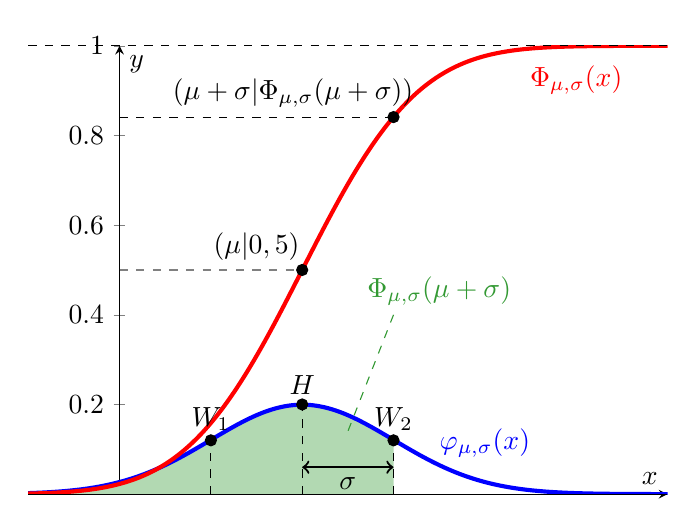
\begin{tikzpicture}
\begin{axis}[%
  axis lines = middle,
  xmajorticks=false,
  xlabel=$x$,
  ylabel=$y$,
  % grid=major,
  xmin=-2, xmax=12,
  width=.8\textwidth,
  height=.6\textwidth,
  % legend pos=north west,
  ]
  \addplot [samples=400, blue, domain=-2:12, line width=1.5pt, name path=normal] {normal(x,4,2)};
  \node at (axis cs:8,0.06) [above, blue] {$\varphi_{\mu, \sigma}(x)$};
  \addplot [samples=400, red, domain=-2:12, line width=1.5pt] {normcdf(x,4,2)};
  \node at (axis cs:10,0.87) [above, red] {$\Phi_{\mu, \sigma}(x)$};
 
  % Wendepunkte markieren 
  \addplot[dashed, black] coordinates {(2,0) (2,0.12)};
  \addplot[dashed, black] coordinates {(6,0) (6,0.12)};
  \addplot[only marks, mark=*] coordinates {(2, 0.12)};
  \addplot[only marks, mark=*] coordinates {(6, 0.12)};
  
  % Wendepunkte Bezeichnung
  \node at (axis cs:4-2,0.12) [above] {$W_1$};
  \node at (axis cs:4+2,0.12) [above] {$W_2$};
  
  % Hochpunkt markieren 
  \addplot[only marks, mark=*] coordinates {(4, 0.2)};
  \addplot[dashed, black] coordinates {(4,0) (4,0.2)};
  % Hochpunkt Bezeichnung
  \node at (axis cs:4,0.2) [above] {$H$};
  
  % Abstand Standardabweichung 
  \draw[<->, thick] 
(axis cs:4,0.06) -- (axis cs:6,0.06)
node[midway, below] {$\sigma$};

  % Erwartungswert der cdf-Funktion markieren
  \addplot[only marks, mark=*] coordinates {(4, 0.5)};
  \node at (axis cs:3,0.5) [above] {$(\mu | \num{0,5})$};
  \addplot[dashed, gray] coordinates {(0,0.5) (4,0.5)};
  
  % Punkt bei Mu + Sigma
  \addplot[only marks, mark=*] coordinates {(6, 0.841)};
  \node at (axis cs:3.8,0.841) [above] {$(\mu+\sigma | \Phi_{\mu, \sigma}(\mu + \sigma))$};
  \addplot[dashed, black] coordinates {(0,0.841) (6,0.841)};
  
% x-Achse als zweite Kurve
\addplot[name path=xaxis, domain=-2:12] {0};
\addplot[domain=-2:12, dashed] {1};

% Fläche zwischen Normalverteilung und x-Achse
\addplot[
    Green!30,
] fill between[
    of=normal and xaxis,
    soft clip={domain=-2:6},
];  

\addplot[dashed, Green!80] coordinates {(6,0.4) (5,0.14)};
\node at (axis cs:7,0.4) [above, Green!80] {$\Phi_{\mu, \sigma}(\mu + \sigma)$};
  
\end{axis}
\end{tikzpicture}
\end{center}

\begin{itemize}
\item Die Wendepunkte $W_1$ und $W_2$ liegen stets bei $x=\mu \pm \sigma$ und der Hochpunkt $H$ von $\varphi_{\mu, \sigma} (x)$ ist bei $x=\mu$.
\item Für die Integralfunktion $\Phi_{\mu, \sigma} (x)$ gilt dabei stets $\Phi_{\mu, \sigma} (\mu)=\num{0,5}$.
\item Für $x\to +\infty$ gilt: $\displaystyle \lim\limits_{x\to +\infty} \Phi_{\mu, \sigma} (x) = \int_{-\infty}^{+\infty} \varphi_{\mu, \sigma} (t) \diff t = 1$. Die Integralfunktion konvergiert also gegen 1. Das bedeutet, dass die Fläche zwischen Gauß'scher Glockenkurve und x-Achse den Wert 1 hat.
\item Nach Definition \ref{Def:Dichtefunktion} ist die Gauß'sche Glockenkurve also eine \textbf{Dichtefunktion}.
\end{itemize}

\index{Gauß'sche Glockenkurve}
\end{definition}

\begin{example}
Gegeben sei eine Funktion $\varphi(x)=\dfrac{1}{\sqrt{8\pi}}e^{-\frac{(x-4)^2}{8}}$. Um daraus die Parameter $\mu$ und $\sigma$ zu bestimmen, kann man wiefolgt vorgehen:
\begin{itemize}
\item $\mu$ ist nur im Zähler des Exponenten gegeben. Wir lesen also $\mu = 4$ ab.
\item $\sigma$ ist laut Definition der Gauß'schen Glockenkurve im Nenner des Exponenten, aber auch im Nenner des Vorfaktors gegeben. Der Vorfaktor bietet sich meistens an, denn dort ist $\sigma$ nicht im Quadrat gegeben. \par
Der Term $\dfrac{1}{\sqrt{8\pi}}$ muss dafür umgeformt werden:
\[ \dfrac{1}{\sqrt{8\pi}} = \dfrac{1}{\sqrt{4\cdot (2\pi)}} = \dfrac{1}{\sqrt{4} \cdot \sqrt{2\pi}} = \dfrac{1}{2\sqrt{2\pi}} \Rightarrow \sigma = 2  \]
\end{itemize}
Somit ist ein lokales Maximum bei $x=4$ und die Wendepunkt sind bei $x=4\pm 2$.
\end{example}

Die Gauß'sche Glockenkurve ist eine wichtige Funktion in der Stochastik, da viele Zufallsgrößen durch sie beschrieben können. Ist das der Fall, so spricht man von einer Normalverteilung:

\begin{definition} \textbf{(Normalverteilung)} \par
Eine Zufallsgröße $X$ heißt \textbf{normalverteilt}, wenn ihre Dichtefunktion eine Gauß'sche Glockenkurve mit den Parametern $\mu$ und $\sigma$ ist. Die Wahrscheinlichkeit dafür, dass $X$ Werte aus dem Intervall $[a,b]$ annimmt, kann durch die kumulative Verteilungsfunktion $\Phi (x)$ beschrieben werden. Es gilt:
\[ P(a\leq X \leq b)=\int_a^b \varphi_{\mu , \sigma} \diff x = \Phi(b) - \Phi(a)  \]
Man sagt, eine Zufallsgröße ist nach $N_{\mu, \sigma}$ verteilt.
\index{Normalverteilung}
\end{definition}

\begin{example}
Oftmals soll man zu gegebenen Normalverteilungen die Kenngrößen $\mu$ und $\sigma$ grafisch bestimmen. Hierzu geht man so vor, dass man bei gegebenen Normalverteilungen den Hochpunkt für die Bestimmung des Erwartungswertes nutzt. Die Entfernung von der Extremstelle zu einer Wendestelle ist dabei stets die Standardabweichung. Ist nur die kumulative Verteilungsfunktion gegeben, so ist für $y=\num{0,5}$ der dazugehörige x-Wert der Erwartungswert. Für die Standardabweichung kann man beispielsweise mithilfe der Sigma-Regeln passende Wahrscheinlichkeitsintervalle bestimmen. Beispielhaft sind für die gegebenen Normalverteilungen

\begin{center}
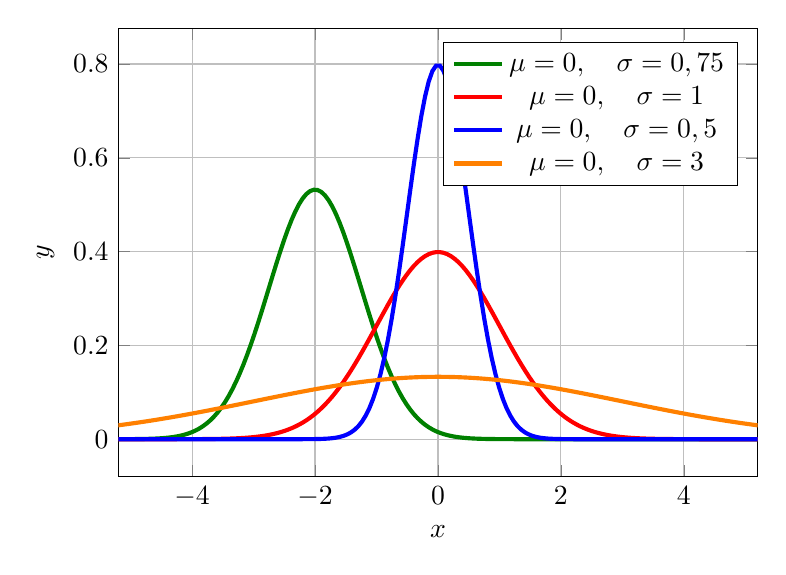
\begin{tikzpicture}
\begin{axis}[%
  xlabel=$x$,
  ylabel=$y$,
  grid=major,
  xmin=-5.2, xmax=5.2,
  width=.8\textwidth,
  height=.6\textwidth,
  legend pos=north east,
  ]
  \addplot [samples=200, Green, domain=-6:6, line width=1.5pt] {normal(x,-2,0.75)};
  \addlegendentry{$\mu = 0, \quad \sigma = \num{0,75}$}
  
  \addplot [samples=200, red, domain=-6:6, line width=1.5pt] {normal(x,0,1)};
  \addlegendentry{$\mu = 0, \quad \sigma = 1$}
  
  \addplot [samples=200, blue, domain=-6:6, line width=1.5pt] {normal(x,0,0.5)};
  \addlegendentry{$\mu = 0, \quad \sigma = \num{0,5}$}
  
  \addplot [samples=200, orange, domain=-6:6, line width=1.5pt] {normal(x,0,3)};
  \addlegendentry{$\mu = 0, \quad \sigma = 3$}
\end{axis}
\end{tikzpicture}
\end{center}

die kumulativen Verteilungsfunktionen gegeben durch

\begin{center}
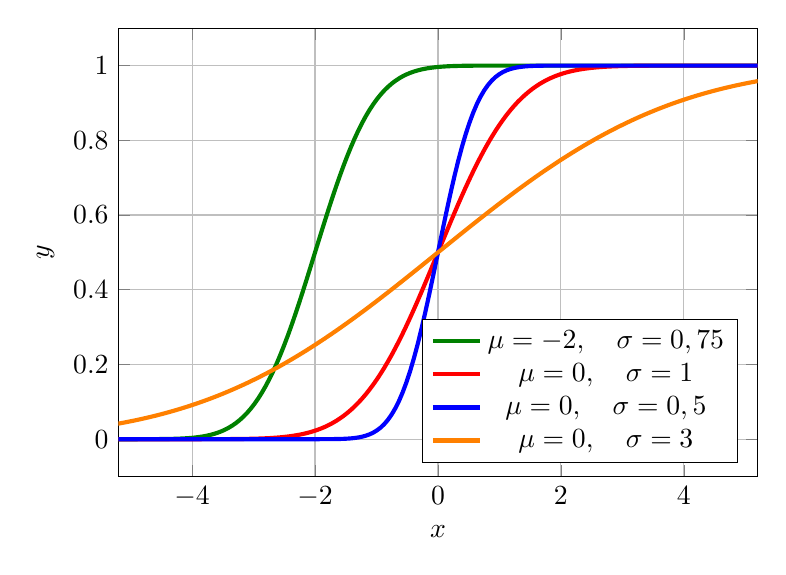
\begin{tikzpicture}
\begin{axis}[%
  xlabel=$x$,
  ylabel=$y$,
  grid=major,
  xmin=-5.2, xmax=5.2,
  width=.8\textwidth,
  height=.6\textwidth,
  legend pos=south east,
  ]
  \addplot [samples=200, Green, domain=-6:6, line width=1.5pt] {normcdf(x,-2,0.75)};
  \addlegendentry{$\mu = -2, \quad \sigma = \num{0,75}$}
  
  \addplot [samples=200, red, domain=-6:6, line width=1.5pt] {normcdf(x,0,1)};
  \addlegendentry{$\mu = 0, \quad \sigma = 1$}
  
  \addplot [samples=200, blue, domain=-6:6, line width=1.5pt] {normcdf(x,0,0.5)};
  \addlegendentry{$\mu = 0, \quad \sigma = \num{0,5}$}
  
  \addplot [samples=200, orange, domain=-6:6, line width=1.5pt] {normcdf(x,0, 3)};
  \addlegendentry{$\mu = 0, \quad \sigma = 3$}
\end{axis}
\end{tikzpicture}

\end{center}



\end{example}

Ist eine Zufallsgröße normalverteilt, so kann man für bestimmte Intervalle die Wahrscheinlichkeiten angeben. Da der Erwartungswert der Hochpunkt ist, und die Normalverteilung um diesen Erwartungswert herum symmetrisch ist, kann man beispielsweise die Wahrscheinlichkeit, dass $X$ einen Wert \textbf{maximal} eine Standardabweichung um den Erwartungswert herum annimmt, stets angeben, ohne, dass man $\mu$ kennen muss. Diese Erkenntnis führt uns zu den Sigma-Regeln:

\begin{theorem} \textbf{(Sigma-Regeln)} \par
\renewcommand{\arraystretch}{1.3}
\begin{center}
\begin{tabular}{c c}
\toprule
Intervall & Wahrscheinlichkeit \\
\midrule
$[\mu-\sigma, \mu + \sigma]$ & $\approx \SI{68,3}{\percent}$ \\
$[\mu-2\sigma, \mu + 2\sigma]$ & $\approx \SI{95,4}{\percent}$ \\
$[\mu-3\sigma, \mu + 3\sigma]$ & $\approx \SI{99,7}{\percent}$ \\
\midrule
$[\mu- \num{1,64} \sigma, \mu + \num{1,64} \sigma]$ & $\approx \SI{90,0}{\percent}$ \\
$[\mu- \num{1,96} \sigma, \mu + \num{1,96} \sigma]$ & $\approx \SI{95,0}{\percent}$ \\
$[\mu- \num{2,58} \sigma, \mu + \num{2,58} \sigma]$ & $\approx \SI{99,0}{\percent}$ \\
\bottomrule
\end{tabular}
\end{center}
\renewcommand{\arraystretch}{1}	
\index{Sigma-Regeln}
\end{theorem}

Mit der oben genannten Symmetrie zu $x=\mu$ lassen sich auch weitere Wahrscheinlichkeiten berechnen.

\begin{example} \ 
\begin{enumerate}
\item Sei eine Zufallsgröße $N_{100, \num{6,5}}$ verteilt. Ist nun nach dem $2\sigma$-Intervall gefragt, so ermitteln wir ihn durch $\mu \pm 2\cdot \sigma$. Also ist der gesuchte Intervall 
\[ [100-13, 100+13] = [87,113]  \]
Es gilt $P(87\leq X \leq 113) \approx \SI{95,4}{\percent}$. Durch die Symmetrie gilt weiterhin
\[ P(87 \leq X \leq 100) = P(100 \leq X \leq 113) \approx \SI{95,4}{\percent} \cdot \dfrac{1}{2} = \SI{47,7}{\percent}  \]

\item Sei nun eine Zufallsgröße mit Erwartungswert $\mu=314$ gegeben. Geben Sie einen Intervall an, in dem die Zufallsgröße zu $\SI{99,0}{\percent}$ liegt. \par
Hierfür betrachten wir die Sigmaregeln. Es gilt $P(\mu - \num{2,58} \sigma \leq X \leq \mu + \num{2,58} \sigma) \approx \SI{99,0}{\percent}$. In abhängigkeit von $\sigma$ lautet eine Lösung für einen Intervall also:
\[ I=[314-\num{2,58}\sigma, 314+\num{2,58}\sigma]\]
\end{enumerate}
\end{example}

\newpage
\section{Symbole und Notationen}
\subsection{Mengen, Mengensymbole und Logik}
\renewcommand{\arraystretch}{1.3}
\begin{tabularx}{\textwidth}{p{2cm} p{6.5cm} X}
Symbol & Begriff & Beispiel\\
\toprule
$M=\{ \}$ & Menge $M$ & $M=\{ 3, 4\}$ ist die Menge, die $3$ und $4$ enthält. \\
$\{ x \in \R | A \}$ & Menge, die alle reellen Zahlen enthält, für die die Eigenschaft $A$ gilt & $\{ x \in \R | a<x<b\}=]a;b[$ ist die Menge, die alle reellen Zahlen zwischen $a$ und $b$ enthält, nicht jedoch $a$ und $b$ selbst (siehe unten). \\
\midrule
$\N$ & Menge der Natürliche Zahlen & $\N=\{0,1,2,\ldots \}$ \\
$\Z$ & Menge der ganzen Zahlen	&	$\Z=\{\ldots , -2,-1,0,1,2, \ldots \}$	\\
$\Q$ & Menge der rationalen Zahlen	&	Alle Zahlen, die man als Bruch aus ganzen Zahlen darstellen kann, sind rational.\\
$\R$ & Menge der reellen Zahlen	& Alle rationalen Zahlen, $-\sqrt{2}$, $\pi$, \ldots	\\
$\R^+$	& Menge der positiven reellen Zahlen & $\sqrt{2}$, $\pi^2$, \ldots	\\
$\R_0^+$ & Menge der nichtnegativen reellen Zahlen & $\R^+$ und die $0$. \\
%\midrule
$[a,b]$ oder $[a;b]$ & (geschlossenes) Intervall & $[-3;2]$ sind alle reellen Zahlen zwischen $-3$ und $2$ (jeweils miteinbegriffen! \\
$]a,b[$ oder $]a;b[$ & (offenes) Intervall & $]-3;2[$ sind alle reellen Zahlen zwischen $-3$ und $2$ (ohne $-3$ und $2$)! \\
\midrule 
$\cap$ & Schnittmenge & $A\cap B$ ist die Menge aller Elemente, die in $A$ und $B$ enthalten sind. \\
$\cup$ & Vereinigungsmenge & $A\cup B$ ist die Menge aller Elemente, die in $A$ oder $B$ enthalten sind (oder in beiden). \\
$\setminus$ & Mengendifferenz & $A\setminus B$ ist die Menge aller Elemente aus $A$, die nicht in $B$ enthalten sind. \\
$\emptyset$ & Leere Menge & Die Menge, die nichts enthält. Alternativ: $\{\}$.\\
$\subset$ & Teilmenge $\N \subset  \R$. & Die natürlichen Zahlen sind eine Teilmenge der reellen Zahlen: Jede natürliche Zahl ist eine reelle Zahl. \\
$\in$ bzw. $\notin$ & (nicht) in einer Menge enthalten & $4\in \N$, aber $\pi \notin \N$. \\
\midrule
$\Rightarrow$ & Folgepfeil (\glqq daraus folgt\grqq ) & $x^2 = 1 \Rightarrow x=\pm1$. Aus $x^2=1$ folgt, dass $x$ entweder $+1$ oder $-1$ ist. \\
$\Leftrightarrow$ & Äquivalenz (\glqq genau dann, wenn\grqq ) & $4=2x \Leftrightarrow 2 = x$. $4=2x$ genau dann, wenn $2=x$ gilt. \\	
\bottomrule
\end{tabularx}
\renewcommand{\arraystretch}{1}	
\subsection{Ausgewählte griechische Buchstaben}
\renewcommand{\arraystretch}{1.3}
\begin{tabularx}{\textwidth}{p{2cm} p{6.5cm} X}
Buchstabe & Name & Beispiel \\
\toprule
$\alpha$ & Alpha & Winkel \\
$\beta$ & Beta & Winkel \\
$\gamma$ & Gamma & Winkel \\
$\lambda$ & Lambda & Parameter in Funktion \\
$\mu$ & My & Erwartungswert \\
$\sigma$ & Sigma & Standardabweichung \\
$\pi$ & Pi & Kreiszahl \\
$\Sigma$ & großes Sigma & Summe: $\sum_{i=1}^n a_i = a_1+a_2 + \ldots + a_n$ \\
$\varphi$, $\phi$ & Phi & Winkel \\
\bottomrule
\end{tabularx}
\renewcommand{\arraystretch}{1}

\subsection{Symbole der Geometrie}
\renewcommand{\arraystretch}{1.3}
\begin{tabularx}{\textwidth}{p{2cm} p{6.5cm} X}
Symbol & Name & Beispiel/Erläuterung \\
\toprule
$A,B,C$ & Punkte & $A(3|4)$ ist ein Punkt im $\R^2$, $B(3|1|4)$ ein Punkt im $\R^3$. \\
$\overline{AB}$ & Strecke & Eine Strecke ist endlich. \\
$|AB|$ & Länge der Strecke & Eine Länge ist nie negativ! \\
$\vv{AB}$ & Vektor & $\vv{AB}=\colvec[1]{1}{4}$ ist ein Vektor. \\
\midrule
$\bot$ & Lot, senkrecht, orthogonal & Ein Normalenvektor ist senkrecht auf seiner Ebene. \\
$\angle ABC$ & Winkel mit Scheitelpunkt $B$ & \\
$\triangle ABC$ & Dreieck mit Punkten $A$, $B$, $C$. & Üblicherweise bezeichnet man die Eckpunkte gegen den Uhrzeigersinn. \\
\bottomrule
\end{tabularx}
\renewcommand{\arraystretch}{1}


% Index soll Stichwortverzeichnis heissen
\renewcommand{\indexname}{Stichwortverzeichnis}
\phantomsection
\pagestyle{skript}
\pagestyle{skript}
% Stichwortverzeichnis soll im Inhaltsverzeichnis auftauchen
\addcontentsline{toc}{section}{Stichwortverzeichnis}

% Stichwortverzeichnis endgueltig anzeigen
\printindex
\thispagestyle{skript}

\end{document}


